\documentclass{article}

\usepackage{libertine}
\usepackage[libertine]{newtxmath}

\usepackage{amsmath}
\usepackage{amsthm}
\usepackage{amssymb}
\usepackage{amsfonts}
\usepackage{graphics}
\usepackage{tikz}
\usepackage{hyperref}
\usepackage{graphicx}
\usepackage{enumerate}
\usepackage{color}
\usepackage{mathtools}
\usepackage{stmaryrd}

\usepackage{pgf, latexsym, float, soul, array, booktabs, dsfont, gensymb, wasysym, multicol, tcolorbox, tabularx, enumitem}

\usepackage{ marvosym }


\usepackage[useregional]{datetime2}

% \renewcommand{\familydefault}{\sfdefault}


\usepackage{fancyheadings}
\pagestyle{fancy}
\cfoot{}
\rfoot{\thepage}
% \lfoot{C$\alpha$lculus}

\fancyhfoffset[r]{\dimexpr2.1in\relax}


\usepackage[margin=1in, right=3in, marginpar=1.9in]{geometry}

% set font encoding for PDFLaTeX, XeLaTeX, or LuaTeX
% \usepackage{ifxetex,ifluatex}
% \if\ifxetex T\else\ifluatex T\else F\fi\fi T%
%   \usepackage{fontspec}
% \else
%   \usepackage[T1]{fontenc}
%   \usepackage[utf8]{inputenc}
%   \usepackage{lmodern}
% \fi


\newcommand{\N}{\mathbb{N}}
\newcommand{\Z}{\mathbb{Z}}
\newcommand{\Zz}{\mathcal{Z}}
\newcommand{\R}{\mathbb{R}}
\newcommand{\Q}{\mathbb{Q}}
\newcommand{\C}{\mathbb{C}}
\newcommand{\PP}{\mathbb{P}}
\newcommand{\X}{\mathcal{X}}
\newcommand{\B}{\mathcal{B}}
\newcommand{\A}{\mathcal{A}}
\newcommand{\M}{\mathcal{M}}
\newcommand{\NN}{\mathcal{N}}
\newcommand{\F}{\mathcal{F}}
\newcommand{\E}{\mathcal{E}}
\newcommand{\ELL}{\mathcal{ELL}}
\renewcommand{\O}{\mathcal{O}}
\renewcommand{\H}{\mathcal{H}}
\newcommand{\D}{\mathbb{D}}
\newcommand{\dabba}{\partial}
\newcommand{\e}{\epsilon}
\newcommand{\eu}{\text{e}}
\newcommand{\bs}{\blacksquare}
\newcommand{\di}{\diamond}
\newcommand{\lb}{\left\lbrace}
\newcommand{\rb}{\right\rbrace}
\newcommand{\on}[1]{\operatorname{#1}}
\newcommand{\lcm}{\on{lcm}}
\newcommand{\multichoose}[2]{\left[#1\atop #2\right]}
\newcommand{\Aut}{\operatorname{Aut}}
\newcommand{\Inn}{\operatorname{Inn}}
\renewcommand{\Im}{\operatorname{Im}}
\newcommand{\Cl}{\operatorname{Cl}}
\newcommand{\Int}{\operatorname{Int}}
\newcommand{\id}{\operatorname{id}}


\newcommand{\mar}[1]{\marginpar{\begin{tcolorbox}[colback=white, arc=0in, left=1mm, right=1mm, leftrule=.3em, bottomrule=.05em, rightrule=.05em, toprule=.05em, halign=flush left]#1\end{tcolorbox}}}




\theoremstyle{definition}
\newtheorem{theorem}{Theorem}[section]
\newtheorem{proposition}[theorem]{Proposition}
\newtheorem{corollary}[theorem]{Corollary}
\newtheorem{lemma}[theorem]{Lemma}

\newtheorem*{theorem*}{Theorem}



\newtheorem*{problem}{Problem}
\newtheorem*{fact}{Fact}
\newtheorem*{claim}{Claim}
\newtheorem*{exercise}{Exercise}

\theoremstyle{definition}
\newtheorem*{definition}{Definition}
\newtheorem*{remark}{Remark}
\newtheorem*{question}{Question}


\newenvironment{thm}[1][]{
\begin{tcolorbox}[colback=white!97!black, arc=0in]
\begin{theorem}[#1]
}{
\end{theorem}
\end{tcolorbox}
}


\newenvironment{strat}[1][]{
\begin{tcolorbox}[colback=white!97!black, arc=0in, title={Strategy: #1}]
}{
\end{tcolorbox}
}





\title{C$\alpha$lculus}
\author{Peter E. Francis}
% \date{}


\begin{document}
% \maketitle
\thispagestyle{empty}

\vspace*{2in}

\begin{Huge}
\noindent C$\alpha$lculus
\end{Huge}

\vspace*{1em}

\noindent Peter E. Francis

\vspace*{5em}

\begin{footnotesize}
\noindent Draft: \DTMnow
\end{footnotesize}

\vfill

\begin{small}
\noindent I would like to thank the following people who have offered suggestions and help putting this together: Keir Lockridge, Samira Arfaee.
\end{small}

\vfill

\noindent Department of Mathematics \\
Stony Brook University\\
Stony Brook, NY 11794, USA, Earth\\

\noindent peter.e.francis@stonybrook.edu

\newpage

\tableofcontents

\newpage



\section*{A Note to Students}
This text is meant to serve as a condensed resource for a student taking their first or second semester of calculus. I am writing with the assumption that the reader is familiar with some trigonometry/pre-calculus, but has perhaps forgotten some of it. While statements I write are always true, they will often not be entirely rigorous or stated with full generality. Use the big margins to make your own notes.  \mar{I'll leave prompts and questions in boxes like this.}

My goal is to communicate what I believe are the key ideas in an introductory calculus class that will help the average student succeed.

Here are my suggestions for doing well in calculus (that should be cyclically repeated!):

\begin{enumerate}
\item Spend time fully understanding key concepts.
\item Identify and learn about common types of problems and exercises.
\item Find some really good examples.
\item Practice a lot!
\end{enumerate}

When you begin learning calculus, it is OK not to understand everything right away. It takes time for some concepts to sink in. Doing a lot of practice will help you start developing intuition about how to tackle new problems, even if you don't fully comprehend everything you are doing. Eventually, your problem-solving skills and your abstract understanding will both be strong, but they need to grow together and build off each other. It is good to sit and actually think about something for a while without doing any writing. Keep at it and eventually you will be able to conjure pictures and animations in your head that relate ideas and succinctly encapsulate the idea of a problem or theorem.


\section*{P.S.}
You might be thinking: ``What the \&\%\$\# is calculus?!''.

Well, let me save you a trip to Wikipedia. At its core, calculus is the study of change. Its name comes from the Latin word for ``pebbles'' because the main idea of calculus is studying things that are changing in non-linear ways by breaking them up into small pieces (like pebbles) that can be thought of as linear, and then putting them back together.

\section*{P.P.S}
Ok... I lied. The pebbles actually refer to the beads on an abacus, but a professor of mine once told me the other version, and I like that better!



\newpage
\part{Pre-Calculus}
\section{Trigonometry}

The word ``trigonometry'' comes from the ancient Greek words for ``triangle'' and ``measure'', and it has found its way into just about every possible branch of mathematics and science. You would be putting yourself at a disadvantage not to make sure you are comfortable with at least the basic ideas of trigonometry before continuing to calculus.

You should think about trigonometry in two ways:
\begin{enumerate}
\item pragmatically (it is a useful tool for solving problems, and there are some things you should memorize)
\item abstractly (it is really just a way to talk about similar triangles)
\end{enumerate}

\subsection{Basic Definitions}
The \textbf{unit circle} is the circle with (unit) radius 1, centered at the origin, $(0,0)$. When we draw a radius of the unit circle, it forms an angle $\theta$ with the positive side of the horizontal axis.

\begin{figure}[h!]
\label{sin-cos-coordinates}
\centering
\begin{tikzpicture}[x=0.75pt,y=0.75pt,yscale=-1,xscale=1]
%uncomment if require: \path (0,300); %set diagram left start at 0, and has height of 300

%Shape: Circle [id:dp4792994212957673]
\draw   (247.5,142.5) .. controls (247.5,86.07) and (293.24,40.33) .. (349.67,40.33) .. controls (406.09,40.33) and (451.83,86.07) .. (451.83,142.5) .. controls (451.83,198.93) and (406.09,244.67) .. (349.67,244.67) .. controls (293.24,244.67) and (247.5,198.93) .. (247.5,142.5) -- cycle ;
%Straight Lines [id:da587287090240175]
\draw    (185.17,142.5) -- (514.17,142.5) ;
%Straight Lines [id:da00739473905145327]
\draw    (350.17,275) -- (349.17,10) ;
%Straight Lines [id:da5956961966671213]
\draw    (349.67,142.5) -- (436.33,89) ;
\draw [shift={(436.33,89)}, rotate = 328.31] [color={rgb, 255:red, 0; green, 0; blue, 0 }  ][fill={rgb, 255:red, 0; green, 0; blue, 0 }  ][line width=0.75]      (0, 0) circle [x radius= 3.35, y radius= 3.35]   ;
%Shape: Arc [id:dp01522092049752044]
\draw  [draw opacity=0] (363.84,133.57) .. controls (365.39,136.03) and (366.32,138.92) .. (366.41,142.03) -- (349.67,142.5) -- cycle ; \draw   (363.84,133.57) .. controls (365.39,136.03) and (366.32,138.92) .. (366.41,142.03) ;
%Straight Lines [id:da14866635901795489]
\draw    (436.33,89) -- (437,142) ;
%Shape: Square [id:dp34042868302746565]
\draw   (430,135) -- (437,135) -- (437,142) -- (430,142) -- cycle ;

% Text Node
\draw (372,129) node [anchor=north west][inner sep=0.75pt]    {$\theta $};
% Text Node
\draw (440,70) node [anchor=north west][inner sep=0.75pt]    {$(\cos \theta ,\ \sin \theta )$};
% Text Node
\draw (385,98) node [anchor=north west][inner sep=0.75pt]    {$1$};
\end{tikzpicture}
\caption{$\sin\theta$ and $\cos\theta$ are coordinates}
\end{figure}

This line segment always has length 1, and connects the origin to some point on the circle. We define $\cos\theta$ and $\sin\theta$ to be the $x$ and $y$ coordinates of this point. In other words, $\cos\theta$ is defined to be the (signed) length of the horizontal leg of the right triangle and similarly, $\sin\theta$ is defined to be the (signed) length of the vertical leg.

We measure angles in either degrees or radians. The angle $\theta$ can be any real number, but there are $2\pi$ radians (or 360\degree) in one full revolution. Imagine the angle $\theta$ changing, making the radius sweep around the circle like a SONAR on a submarine. The hypotenuse of the triangle stays constantly at 1, but the side lengths fluctuate between 1 and 0. \mar{Draw a picture: where on the unit circle is $\cos\theta$ positive and where is it negative? How about $\sin\theta$?}

The two functions $\sin$ and $\cos$ are the basic building blocks, but there are four other commonly used trig functions. They are defined as follows:
$$\sec \theta = \frac{1}{\cos\theta}, \quad \quad \csc\theta=\frac{1}{\sin\theta}, \quad \quad \tan\theta=\frac{\sin\theta}{\cos\theta}, \quad \quad \cot\theta=\frac{\cos\theta}{\sin\theta}.$$
These functions also have visual representations on the unit circle.
\begin{figure}[h!]
\centering
\fbox{
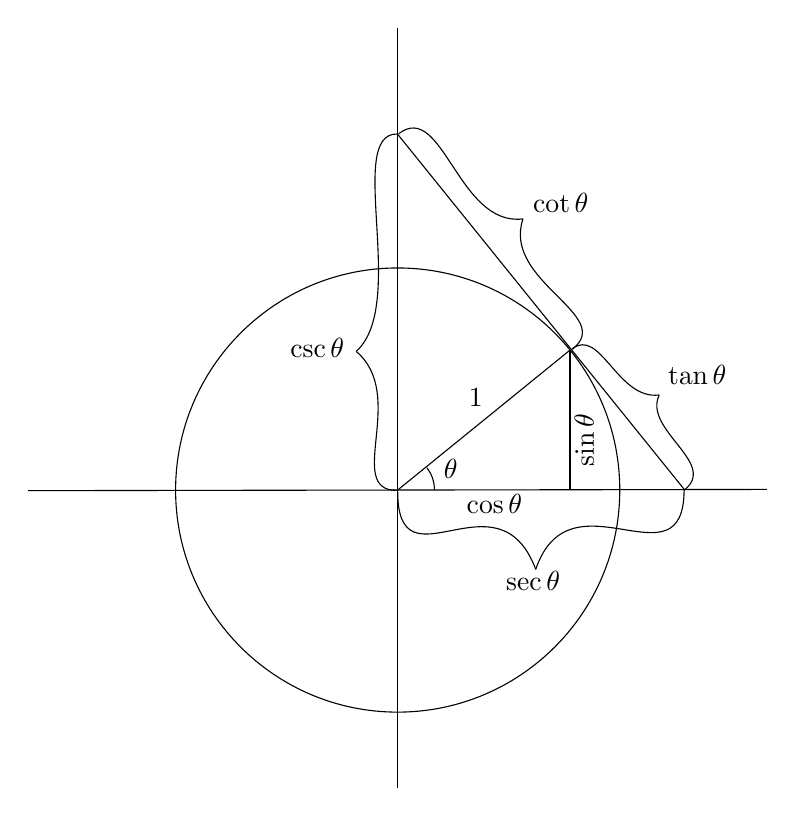
\begin{tikzpicture}[x=0.75pt,y=0.75pt,yscale=-1,xscale=1]
%uncomment if require: \path (0,434); %set diagram left start at 0, and has height of 434

%Shape: Circle [id:dp8118961016990287]
\draw   (214,254.2) .. controls (214,195.11) and (261.91,147.2) .. (321,147.2) .. controls (380.09,147.2) and (428,195.11) .. (428,254.2) .. controls (428,313.29) and (380.09,361.2) .. (321,361.2) .. controls (261.91,361.2) and (214,313.29) .. (214,254.2) -- cycle ;
%Straight Lines [id:da6733376051381585]
\draw    (143,254.5) -- (499,253.9) ;
%Straight Lines [id:da24708595669358502]
\draw    (321,31.7) -- (321,397.7) ;
%Straight Lines [id:da2369525758798794]
\draw    (404,186.8) -- (321,254.2) ;
%Straight Lines [id:da6269364989299404]
\draw    (459,253.8) -- (321,82.8) ;
%Shape: Arc [id:dp8953631465255683]
\draw  [draw opacity=0] (335.11,243.48) .. controls (337.38,246.45) and (338.72,250.17) .. (338.72,254.2) .. controls (338.72,254.26) and (338.72,254.32) .. (338.72,254.39) -- (321,254.2) -- cycle ; \draw   (335.11,243.48) .. controls (337.38,246.45) and (338.72,250.17) .. (338.72,254.2) .. controls (338.72,254.26) and (338.72,254.32) .. (338.72,254.39) ;
%Straight Lines [id:da9446390224381691]
\draw    (404,186.8) -- (404,253.8) ;
%Curve Lines [id:da6889044659660293]
\draw    (321,254.85) .. controls (321,303.53) and (369.22,243.72) .. (387.51,292.4) ;
%Curve Lines [id:da7744827450838345]
\draw    (387.51,292.4) .. controls (404.13,243.72) and (459,302.6) .. (459,253.92) ;
%Curve Lines [id:da7475604962570235]
\draw    (320.73,82.66) .. controls (295.65,82.31) and (326.19,164.99) .. (301,187.4) ;
%Curve Lines [id:da536698622904964]
\draw    (301,187.4) .. controls (325.99,208.44) and (295.33,254.05) .. (320.41,254.4) ;
%Curve Lines [id:da3819978579463683]
\draw    (405.09,186.4) .. controls (426.34,170.03) and (371.15,153.75) .. (381.37,123.57) ;
%Curve Lines [id:da6758383716021474]
\draw    (381.37,123.57) .. controls (350.09,127.39) and (342.7,66.17) .. (321.45,82.55) ;
%Curve Lines [id:da9285330284788131]
\draw    (458.84,254.4) .. controls (476,241.4) and (439,225.4) .. (447,208.4) ;
%Curve Lines [id:da5181742767873634]
\draw    (447,208.4) .. controls (426.87,210.91) and (418.68,175.48) .. (405,186.23) ;

% Text Node
\draw (342,238) node [anchor=north west][inner sep=0.75pt]    {$\theta $};
% Text Node
\draw (372,292) node [anchor=north west][inner sep=0.75pt]   [align=left] {$\displaystyle \sec \theta $};
% Text Node
\draw (268,180) node [anchor=north west][inner sep=0.75pt]   [align=left] {$\displaystyle \csc \theta $};
% Text Node
\draw (385,110) node [anchor=north west][inner sep=0.75pt]   [align=left] {$\displaystyle \cot \theta $};
% Text Node
\draw (450,193) node [anchor=north west][inner sep=0.75pt]   [align=left] {$\displaystyle \tan \theta $};
% Text Node
\draw (353,255) node [anchor=north west][inner sep=0.75pt]   [align=left] {$\displaystyle \cos \theta $};
% Text Node
\draw (405,244) node [anchor=north west][inner sep=0.75pt]  [rotate=-270] [align=left] {$\displaystyle \sin \theta $};
% Text Node
\draw (354,204) node [anchor=north west][inner sep=0.75pt]   [align=left] {$1$};


\end{tikzpicture}
}
\caption{The six common trig functions on the unit circle}
\label{6trig}
\end{figure}


To explore these functions, check out \href{https://www.desmos.com/calculator/fdr54f2jh3}{this graph on Desmos}.


\subsection{Values on the Unit Circle}

There are several angles $\theta$ for which you should be able to compute $\sin\theta$ and $\cos\theta$ (then computing the other four trig functions is easy). Luckily, there is a lot of symmetry involved: it is only necessary to memorize a few numbers and then you can easily fill in the rest.

Below is a diagram of all of the angles whose $\sin$ and $\cos$ you should be familiar with.

\begin{figure}[h!]
\label{the-unit-circle}
\centering
\fbox{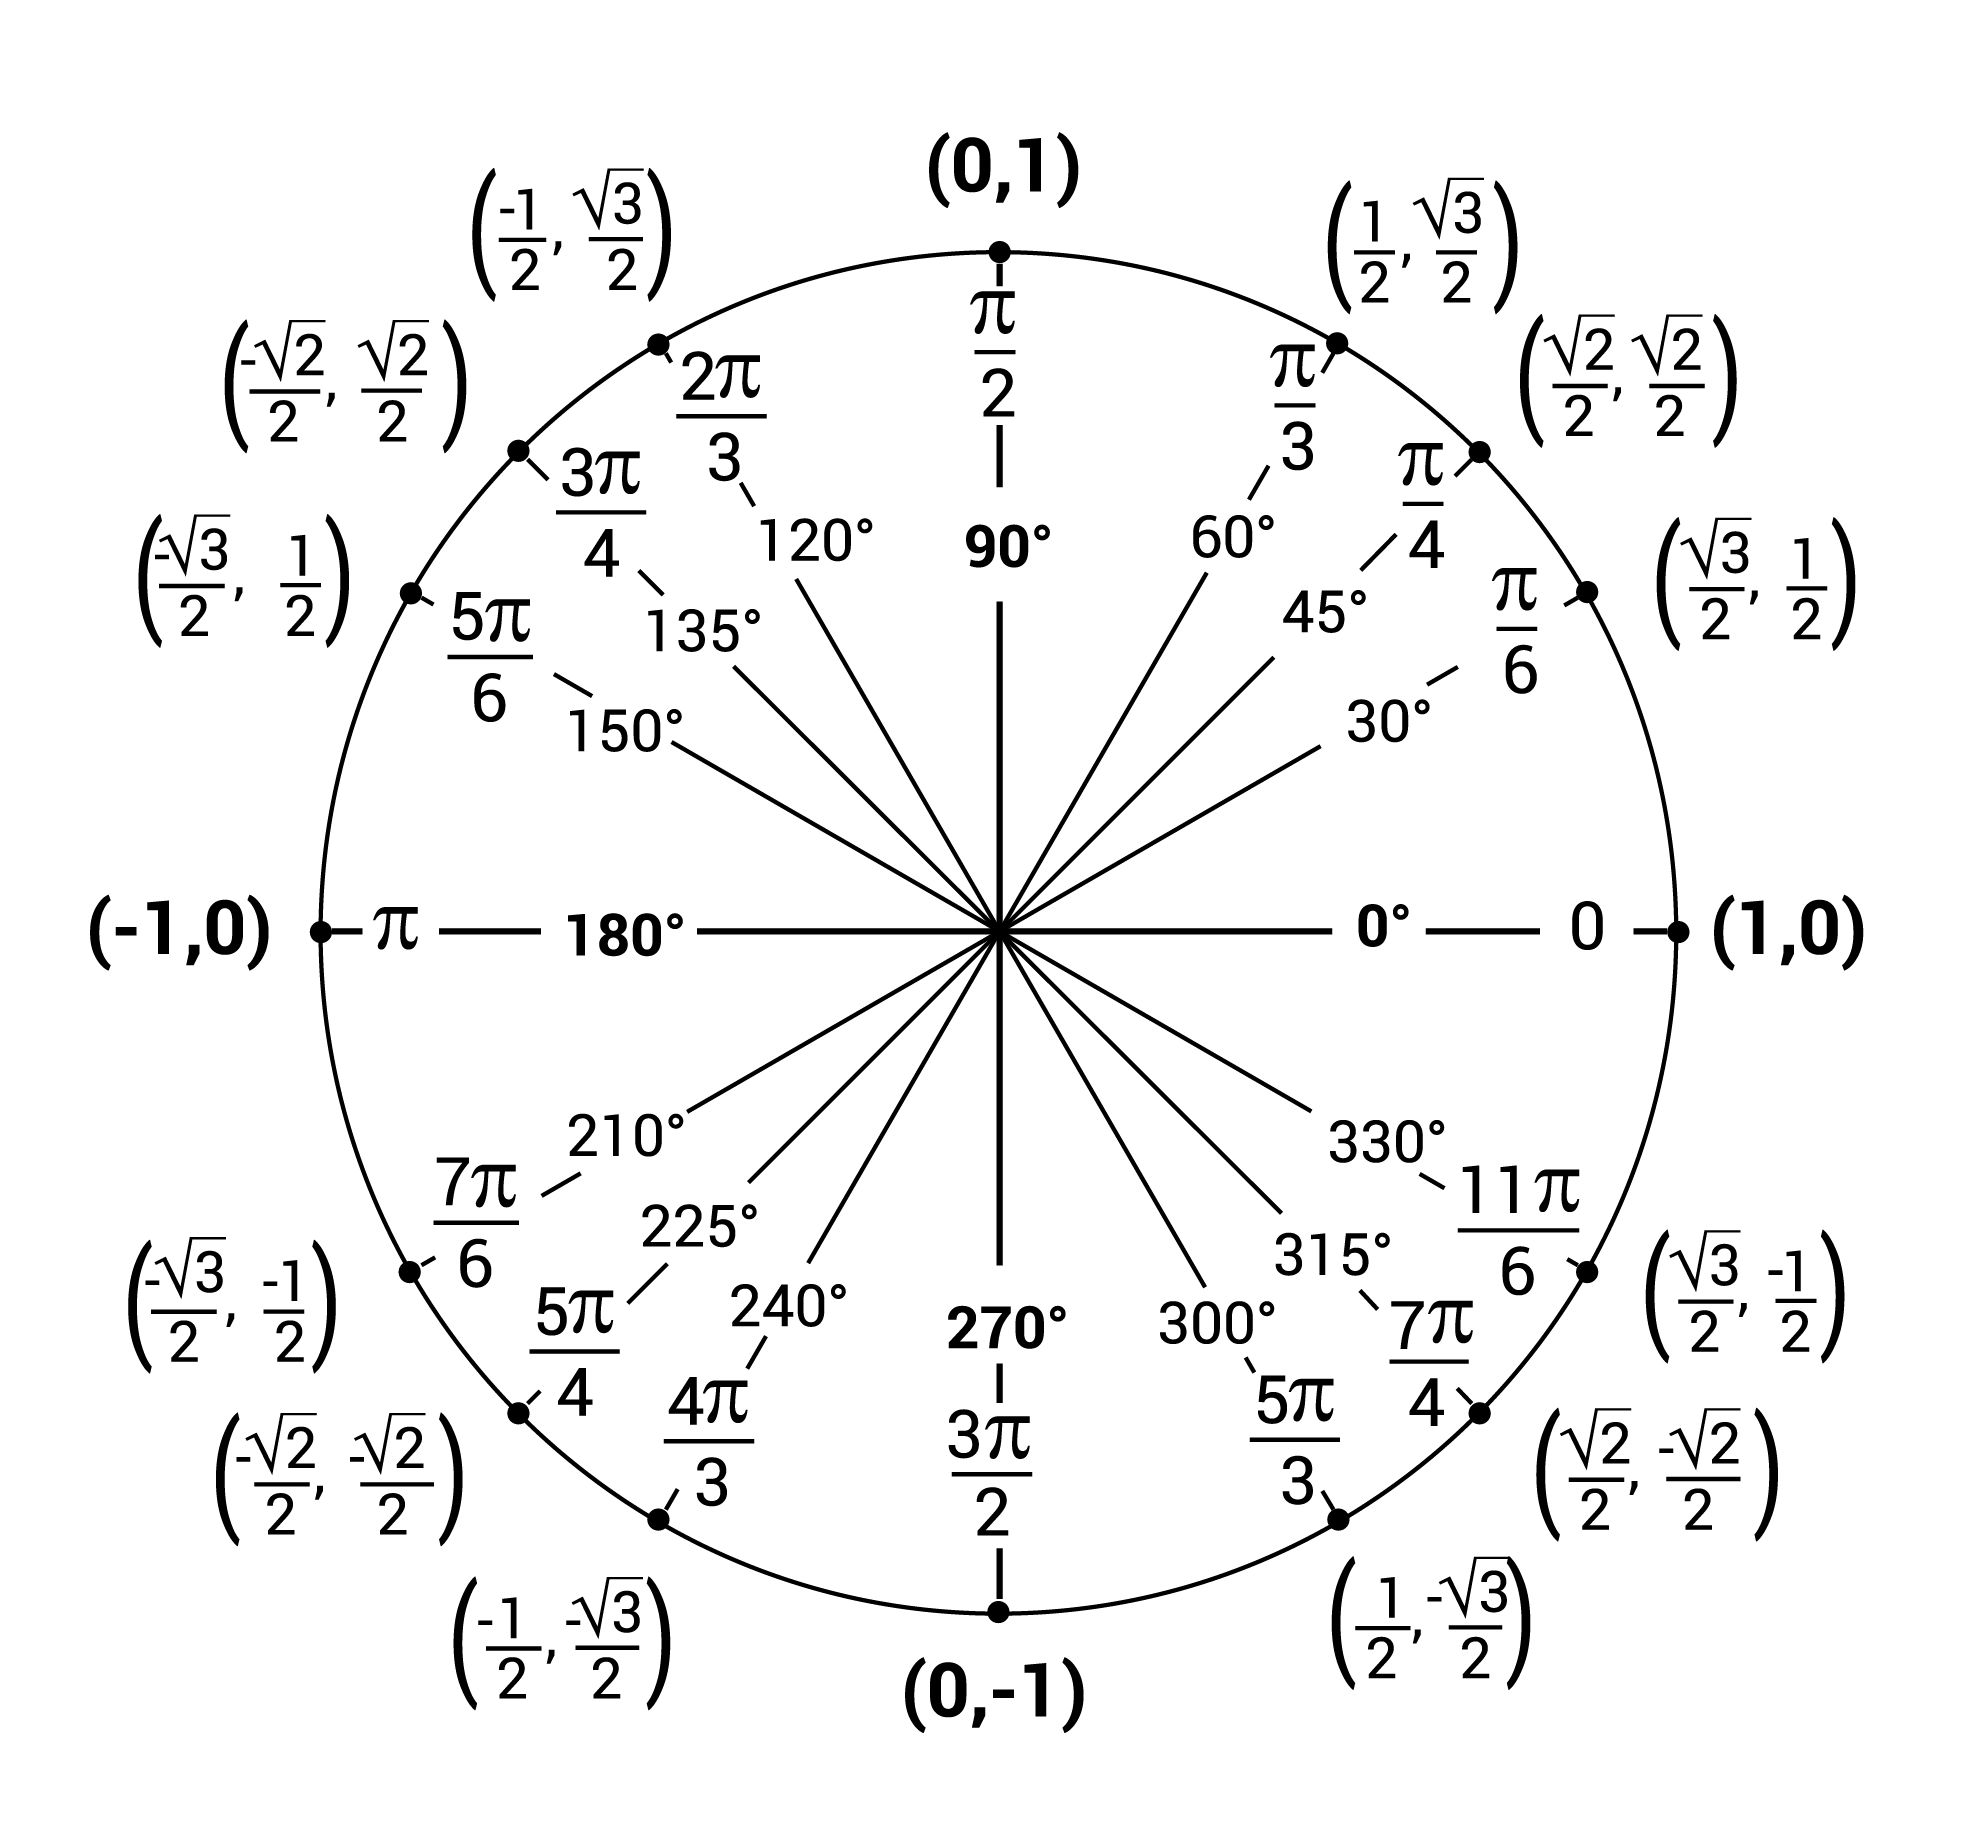
\includegraphics[width=4in]{img/unit-circle.png}}
\caption{The Unit Circle}
\end{figure}


It might seem intimidating, but just focus on the first (upper-right) quadrant and the first five angles there:


\begin{center}
\renewcommand{\arraystretch}{1.3}
\begin{tabular}{@{}lll@{}}
\toprule[0.4mm]
$\theta$ & $\cos\theta$ & $\sin\theta$ \\\midrule
   $0$  & $\sqrt{4}/2$ & $\sqrt{0}/2$ \\
$\pi/6$ & $\sqrt{3}/2$ & $\sqrt{1}/2$ \\
$\pi/4$ & $\sqrt{2}/2$ & $\sqrt{2}/2$ \\
$\pi/3$ & $\sqrt{1}/2$ & $\sqrt{3}/2$ \\
$\pi/2$ & $\sqrt{0}/2$ & $\sqrt{4}/2$ \\\bottomrule[0.4mm]
\end{tabular}
\end{center}

In this table, I wrote the numbers in an ``un-simplified'' way so you can see the pattern: their numerators change by 1 under a square-root, and as one goes up, the other goes down.

You can also see that the values for other angles are the same number, but with a different sign (according to the quadrant they are in), and that the unit circle is symmetric, reflecting over the $x$ and $y$ axis.

\subsection{The Pythagorean and Other Identities}

Remember the Pythagorean Theorem, $a^2 + b^2 = c^2$? Well, since $\sin\theta$ and $\cos\theta$ are the lengths of a right triangle with hypotenuse 1, we have the following \textbf{Pythagorean identity}:
$$\cos^2\theta +\sin^2\theta = 1.$$
\mar{Which of the following are the same?
\begin{center}
\begin{tabular}{ c c }
$\sin\theta^2$ & $\sin^2\theta$ \\
$\sin(\theta^2)$ & $\sin(\theta)^2$ \\
$(\sin(\theta))^2$ & $(\sin\theta)^2$ \\
\end{tabular}
\end{center}
}
Dividing this equation by $\sin^2\theta$ or $\cos^2\theta$, we get
$$\cot^2\theta + 1 = \csc^2\theta\quad\quad\text{and}\quad\quad 1+\tan^2\theta = \sec^2\theta.$$

There is some nice symmetry between $\sin\theta$ and $\cos\theta$. The leg opposite the angle is $\theta$ is $\sin\theta$. Since the internal angles of a triangle sum to $\pi$, the other acute angle is $\frac{\pi}{2} - \theta$. \mar{Label the angle $\frac{\pi}{2}-\theta$ on Figure \ref{sin-cos-coordinates}.} Then, the leg opposite $\frac{\pi}{2} - \theta$ has length $\sin\left(\frac{\pi}{2} - \theta\right)$, but is also $\cos\theta$. Therefore,
$$\sin\left(\frac{\pi}{2} - \theta\right) = \cos(\theta).$$
Similarly,
$$\cos\left(\frac{\pi}{2} - \theta\right) = \sin(\theta).$$
Looking at the picture of the unit circle, we can also see that
$$\sin(-\theta) = -\sin(\theta)\quad\text{and}\quad \cos(-\theta)=\cos(\theta).$$

There is one more kind of identity that will be useful for us:
$$\sin(A\pm B)=\sin A \cos B \pm \cos A \sin B,$$
$$\cos(A\pm B)=\cos A \cos B \mp \sin A \sin B.$$

These are called the \textbf{angle sum formulas}, and they are long but if you read them out loud, they make a little song! Try it while clapping on each word:
\begin{center}
``SINE-COSINE-COSINE-SINE. COSINE-COSINE-SINE-SINE.''
\end{center}\mar{No seriously, sing the song. Now do it again.}
Once you remember the order of the functions, you just have to remember that the $A$s and $B$s alternate and that the sign in the second equation flips ($\pm$ becomes $\mp$).

These simplify if $A$ and $B$ are the same angle $\theta$ to what are called the \textbf{double angle formulas}. In this case,
$$\sin(2\theta) = 2\sin\theta\cos\theta$$
and
\begin{align*}
\cos(2\theta) & = \cos^2\theta - \sin^2\theta \\
              & = 1 - 2\sin^2\theta \\
              & = 2\cos^2\theta - 1.
\end{align*}
\mar{Check that these are correct. Hint: use the Pythagorean identity.}

\subsection{Applications}

So, how do we use trigonometry to help solve problems? The main way that trigonometry is useful for you as a calculus student is two-fold. One is as a source of nice function examples to play around with (once we start taking limits and derivatives). The other is as a means to fill in missing information (this is the ``SOH-CAH-TOA'' you might remember).

Let's say you have a right triangle with hypotenuse 8 and one a $30\degree$ angle.


\begin{figure}[h!]
\centering
\tikzset{every picture/.style={line width=0.75pt}} %set default line width to 0.75pt
\fbox{\begin{tikzpicture}[x=0.75pt,y=0.75pt,yscale=-1,xscale=1]
%uncomment if require: \path (0,300); %set diagram left start at 0, and has height of 300

%Shape: Right Triangle [id:dp06753223391248242]
\draw   (236,78) -- (62.56,189.5) -- (236,189.5) -- cycle ;
%Shape: Arc [id:dp8301261755391214]
\draw  [draw opacity=0] (84.77,175.15) .. controls (87.45,179.28) and (89,184.21) .. (89,189.5) -- (62.56,189.5) -- cycle ; \draw   (84.77,175.15) .. controls (87.45,179.28) and (89,184.21) .. (89,189.5) ;
%Shape: Rectangle [id:dp7819843676440785]
\draw   (222.88,176.38) -- (236,176.38) -- (236,189.5) -- (222.88,189.5) -- cycle ;
%Shape: Right Triangle [id:dp36110349096513206]
\draw   (460.53,102) -- (358.65,167.49) -- (460.53,167.49) -- cycle ;
%Shape: Arc [id:dp10101111854625855]
\draw  [draw opacity=0] (371.7,159.07) .. controls (373.27,161.49) and (374.18,164.39) .. (374.18,167.49) -- (358.65,167.49) -- cycle ; \draw   (371.7,159.07) .. controls (373.27,161.49) and (374.18,164.39) .. (374.18,167.49) ;
%Shape: Rectangle [id:dp8285259686836064]
\draw   (452.83,159.79) -- (460.53,159.79) -- (460.53,167.49) -- (452.83,167.49) -- cycle ;
%Curve Lines [id:da345399705785322]
\draw    (268,78) .. controls (303.46,52.98) and (335.04,54.55) .. (366.56,76.96) ;
\draw [shift={(368,78)}, rotate = 216.18] [color={rgb, 255:red, 0; green, 0; blue, 0 }  ][line width=0.75]    (10.93,-3.29) .. controls (6.95,-1.4) and (3.31,-0.3) .. (0,0) .. controls (3.31,0.3) and (6.95,1.4) .. (10.93,3.29)   ;

% Text Node
\draw (90.25,173) node [anchor=north west][inner sep=0.75pt]    {$30\degree $};
% Text Node
\draw (136,124.4) node [anchor=north west][inner sep=0.75pt]    {$8$};
% Text Node
\draw (144,192) node [anchor=north west][inner sep=0.75pt]    {$x$};
% Text Node
\draw (238,130) node [anchor=north west][inner sep=0.75pt]    {$y$};
% Text Node
\draw (377,154) node [anchor=north west][inner sep=0.75pt]    {$30\degree $};
% Text Node
\draw (398,125) node [anchor=north west][inner sep=0.75pt]    {$1$};
% Text Node
\draw (401,169) node [anchor=north west][inner sep=0.75pt]    {$x/8$};
% Text Node
\draw (461,125) node [anchor=north west][inner sep=0.75pt]    {$y/8$};
% Text Node
\draw (301,42) node [anchor=north west][inner sep=0.75pt]    {$\div 8$};


\end{tikzpicture}}
\caption{Similar Triangles}
\end{figure}

If you want to know what the other side lengths are, this is how you can use trigonometry to do it! First, scale the triangle down by the side length that you know (in this case $8$). This doesn't change the angles, so we now have a right triangle with hypotenuse 1. By definition of $\sin$ and $\cos$,
$$\sin 30\degree = \frac{y}{8}\quad\quad\text{and}\quad\quad\cos 30\degree=\frac{x}{8},$$
so we can solve for $x$ and $y$:
$$y = 8\sin 30\degree = 4\quad\quad\text{and}\quad\quad x= 8\cos 30\degree= 4\sqrt{3}.$$
The mnemonic device ``SOH-CAH-TOA'' reminds us that \underline{S}in of $30\degree$ is the \underline{O}pposite leg ($y$) over the \underline{H}ypotenuse (8), and \underline{C}os of $30\degree$ is the \underline{A}djacent leg ($x$) over the \underline{H}ypotenuse (8). \mar{What does the ``TOA'' part say? What situation would it help you figure something out about a triangle?}

The identities that we learned about also have many applications, but mostly are in simplifying calculuations. You should keep them in mind so you recognize when they might be helpful in simplifying an expression. Here is a cool example:
\begin{align*}
\sin\left(2\theta\right)\left(\frac{\tan \theta+\cot \theta}{2}\right)
& = 2\sin\theta\cos\theta\left(\frac{\frac{\sin\theta}{\cos\theta}+\frac{\cos\theta}{\sin\theta}}{2}\right)\\
& = \sin\theta\cos\theta\left(\frac{\sin\theta}{\cos\theta}+\frac{\cos\theta}{\sin\theta}\right)\\
& = \sin^2\theta+\cos^2\theta\\
& = 1.
\end{align*}


Trig identities can also be a computationally useful tool: if you need to know the Sine (or Cosine, etc.) of an angle you are not familiar with, write the angle as a sum or difference of angles you know and use the angle sum formulas. For example,
\begin{align*}
\cos(15\degree) & = \cos(45\degree-30\degree) \\
                & = \cos(45\degree)\cos(30\degree)+\sin(45\degree)\sin(30\degree) \\
                & = \frac{\sqrt{2}}{2}\frac{\sqrt{3}}{2} + \frac{\sqrt{2}}{2}\frac{1}{2} \\
                & = \frac{\sqrt{6}+\sqrt{2}}{4}.
\end{align*}
\mar{Can you compute $\tan(75\degree)$?}

\subsection{There's Always More Trigonometry...}

Trigonometry dates back to the 3rd century BCE and needless to say it has changed a bit over the years. We've only covered the basics and focused on the trigonometry involving right triangles. There is always more trigonometry to learn: more trigonometric functions and MANY more relations among them! I won't pester you with many more right now, but they might come up in the future, so just be aware.

The two very common laws of trigonometry that involve non-right triangles are the Law of Sines and the Law of Cosines. I will state them here (for culture).

\begin{figure}[!h]
\centering
\label{circumscribed-triangle}
\tikzset{every picture/.style={line width=0.75pt}} %set default line width to 0.75pt

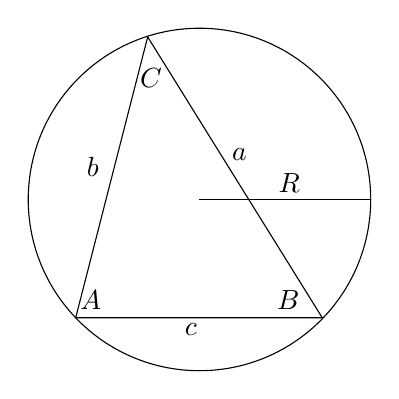
\begin{tikzpicture}[x=0.75pt,y=0.75pt,yscale=-1,xscale=1]
%uncomment if require: \path (0,476); %set diagram left start at 0, and has height of 476

%Shape: Circle [id:dp3720781821561441]
\draw   (155,137.5) .. controls (155,91.94) and (191.94,55) .. (237.5,55) .. controls (283.06,55) and (320,91.94) .. (320,137.5) .. controls (320,183.06) and (283.06,220) .. (237.5,220) .. controls (191.94,220) and (155,183.06) .. (155,137.5) -- cycle ;
%Shape: Triangle [id:dp2721155840135763]
\draw   (212.55,59.19) -- (296.67,194.5) -- (177.87,194.5) -- cycle ;
%Straight Lines [id:da18934326053160722]
\draw    (237.5,137.5) -- (320,137.5) ;

% Text Node
\draw (252,111.82) node [anchor=north west][inner sep=0.75pt]    {$a$};
% Text Node
\draw (178.85,180) node [anchor=north west][inner sep=0.75pt] {$A$};
% Text Node
\draw (273.69,180) node [anchor=north west][inner sep=0.75pt] {$B$};
% Text Node
\draw (207.69,73) node [anchor=north west][inner sep=0.75pt]    {$C$};
% Text Node
\draw (229.18,196) node [anchor=north west][inner sep=0.75pt]    {$c$};
% Text Node
\draw (182,116.07) node [anchor=north west][inner sep=0.75pt]    {$b$};
% Text Node
\draw (274.32,123.82) node [anchor=north west][inner sep=0.75pt]    {$R$};


\end{tikzpicture}
\caption{Circumscribed Triangle}
\end{figure}

Figure \ref{circumscribed-triangle} shows a triangle with internal angles $A$, $B$, and $C$, and respective opposite side lengths $a$, $b$, and $c$. The triangle is \textbf{circumscribed} in a circle, meaning its vertices lie on the circle's boundary. It turns out that the circle has radius
$$R=\frac{abc}{\sqrt{(a+b+c)(a-b+c)(a+b-c)(-a+b+c)}}.$$



\begin{thm}[Law of Sines]
If a triangle has sides and angles as above, then
$$\frac{a}{\sin A}=\frac{b}{\sin B}=\frac{c}{\sin C}=2R=\frac{abc}{2\Delta},$$
where $R$ is the radius of the circumscribed circle and $\Delta$ is the area of the triangle.
\end{thm}

\begin{thm}[Law of Cosines]
If a triangle has sides and angles as above, then
$$a^2+b^2=c^2+2ab\cos C.$$
\end{thm}
\mar{Almost looks familiar, doesn't it?}

When you use these formulas, keep in mind that solving for an angle can be tricky: if $\sin\theta=1/2$, then $\theta$ could be $30\degree$, $150\degree$, $390\degree$, etc..



\newpage
\section{Functions on the Real Line}

\subsection{Real Numbers}

The set of real numbers ($\R$) is an uncountably infinite set, meaning I can not even begin to exhaustively list all of its members. However, here are some of my favorites: $3$, $2/5$, $4.11$, $713$, $\sqrt{37}$, $\pi$. Real numbers include both the rationals and irrationals. \mar{Do you know any numbers that aren't real?}

The real numbers can be thought of as a continuum that has no beginning and no end: real numbers can get infinitely small and infinitely large.

More concretely, imagine you are standing on a road that goes on forever, both in front of you and behind you. If you drop a traffic cone where you are standing, and call it ``the origin'', then any distance you walk on this road away from the cone is a real number. If you walk forward, it is positive, and if you walk backwards, it is negative. You can keep walking forever and reach any number you would like, but you will never reach an ``end of the road'' because it doesn't exist.

\subsection{Subsets of the Real Line}

A \textbf{subset} is a subcollection. There are a few ways we notate subsets of $\R$, so this section is mostly dedicated to notation. The first two examples of a subset are kind of stupid: the \textbf{empty set} $\emptyset$ (the set with no elements), and all of $\R$ are both subsets of $\R$.

You can define a \textbf{literal} subset of $\R$ by listing the elements it contains. For example, $\{1,2,3\}$ is the set containing 1, 2, and 3.

\textbf{Intervals} are---in my opinion---the most important kind of subset of $\R$. The following table shows the 8 kinds of intervals and the two ways we write them ($a\leq b$ are real numbers).

\begin{center}
\renewcommand{\arraystretch}{1.1}
\begin{tabular}{p{3.5in} p{1.25in} p{1.3in}}
\toprule[0.4mm]
The set of real numbers that are... & \textbf{Interval Notation} & \textbf{Set-Builder Notation} \\ \midrule
greater than $a$ and less than $b$ & $(a,b)$ & $\{x\in\R\ :\ a < x < b\}$ \\
greater than or equal to $a$ and less than $b$ & $[a,b)$ & $\{x\in\R\ :\ a \leq x < b\}$ \\
greater than $a$ and less than or equal to $b$ & $(a,b]$ & $\{x\in\R\ :\ a < x \leq b\}$ \\
greater than or equal to $a$ and less than or equal to $b$ & $[a,b]$ & $\{x\in\R\ :\ a \leq x \leq b\}$ \\
greater than $a$ & $(a,\infty)$ & $\{x\in\R\ :\ a < x\}$ \\
greater than or equal to $a$ & $[a,\infty)$ & $\{x\in\R\ :\ a \leq x\}$ \\
less than $b$ & $(-\infty,b)$ & $\{x\in\R\ :\ x < b\}$ \\
less than or equal to $b$ & $(-\infty,b]$ & $\{x\in\R\ :\ x \leq b\}$ \\
\bottomrule
\end{tabular}
\end{center}


Interval notation is easy to write and read, once you get a hang of what the different parentheses mean. The regular parentheses $()$ are called ``open'' and mean that the particular endpoint of the interval is not included. The $[]$ brackets are called ``closed'' and indicate that the endpoint \textit{is} included. \mar{Why aren't $(a,\infty]$, $(a,\infty]$, $[-\infty,b)$, and $[-\infty,b]$ included in the table?}

The set-builder notation is read as follows:

% \vspace*{1em}

\begin{Large}
$$\{\underbrace{x}_x\underbrace{\in}_\text{in}\underbrace{\R}_{\text{the real}\atop \text{numbers}}\ \underbrace{:}_\text{such that}\ \underbrace{a < x < b}_{x\text{ is strictly}\atop\text{between }a\text{ and }b}}\}.$$
\end{Large}

% \vspace*{1em}


All of the subsets of $\R$ that you'll want to use in this course can be written using combinations of intervals. There are two ways to do this:
\begin{itemize}
\item The \textbf{union} of two sets is the set that contains all of the elements in either set and is denoted with the ``cup'' symbol, $\cup$.
\item The \textbf{intersection} of two sets is the set that contains the elements in both sets and is denoted with the ``cap'' symbol, $\cap$.
\end{itemize}
Here are some examples:
\begin{center}
\renewcommand{\arraystretch}{1.1}
\begin{tabular}{@{}l l l l @{}}
\toprule[0.4mm]
$A$ & $B$ & $A\cup B$ & $A\cap B$\\
\midrule
$\{1, 2, 3\}$ & $\{3, 4, 5\}$ & $\{1,2,3,4,5\}$ & $\{3\}$ \\
$\{0, 2, 3\}$ & $(1,3)$ & $\{0\}\cup(1,3]$ & $\{2\}$\\
$(3,4]$ & $[4,5)$ & $(3,5)$ & $\{4\}$ \\
$(-\infty,5)$ & $[5,\infty)$ & $(-\infty,\infty)=\R$ & $\emptyset$ \\
$(-3,0)$ & $(2,6)$ & $(-3,0) \cup (2,6)$ & $\emptyset$ \\
$(1,5)$ & $(3, 7)$ & $(1,7)$ & $(3,5)$ \\
$(1,8)$ & $(3, 4)$ & $(1,8)$ & $(3,4)$ \\
\bottomrule
\end{tabular}
\mar{Draw a picture of each of these examples. Does \textit{Venn diagram} ring any bells?}
\end{center}

\subsection{Defining Functions}

We will start with quite a few new (and abstract) definitions, but we will make things concrete very soon.

If $A$ and $B$ are two sets, a \textbf{function} $f$ from $A$ to $B$ is an assignment of each element of $A$ to a unique element of $B$. In other words, for each input $a$ in $A$, $f$ outputs exactly one $b$ in $B$, which we denote as $f(a)$. The set $A$ is called the \textbf{domain} of $f$, the set $B$ is called the \textbf{codomain} of $f$, and we write $$f:A\to B\quad\quad\text{ or }\quad\quad A\overset{f}{\to} B.$$
Please remember that a function has three pieces of information: the domain, the codomain, and the rule of assignment. If one of these pieces is changed, the resulting function is different. \mar{Is $f$ defined by $$f(x)=\begin{cases}x+1 & x > 0 \\ x^2 & x < 1\end{cases}$$ a function?}

The \textbf{range} of $f$ is the set of all outputs of $f$ and is denoted $f(A)$. The range is always a subset of the codomain, but they are not always equal sets. The relationship between the domain, codomain, and the range are an important one:
\begin{itemize}
\item A function is called \textbf{surjective} (or \textbf{onto}) if its range and codomain are the same (i.e. $f(A)=B$). In other words, a function is surjective if every element of the codomain is an output of $f$. \mar{What does the word ``sur'' mean in French?}
\item A function is called \textbf{injective} (or \textbf{one-to-one}) if each element of the range is the output of exactly one element of the domain. In other words, if $f(x_1)=f(x_2)$, then $x_1=x_2$.
\item If a function is both surjective and injective, then it is called \textbf{bijective}.
\end{itemize}

The figure below is a cartoon of three functions. From left to right, (1) a surjection that is not injective, (2) a bijection, and (3) an injection that is not surjective. \mar{Write down the domain, codomain, and range of each of these functions.}



\begin{figure}[H]
\label{three-functions}
\centering
\fbox{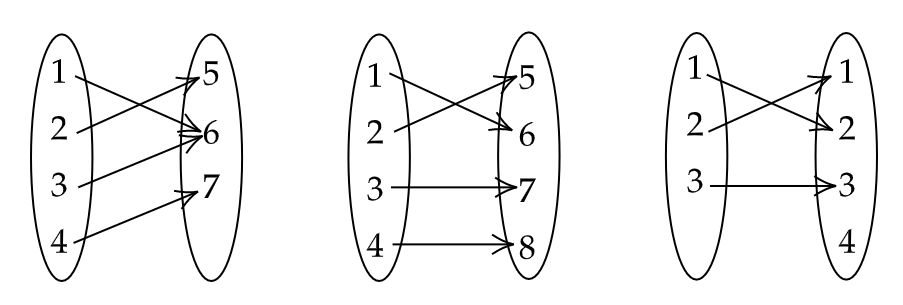
\includegraphics[width=4in]{img/three-functions.png}}
\caption{A Surjection, a Bijection, and an Injection}
\end{figure}


We will only use \textbf{real functions}, which are functions whose domain and codomain are subsets of $\R$. These functions take real numbers as inputs and give real numbers as outputs, so they can be graphed on a Cartesian grid, with the inputs on the horizontal axis and outputs on the vertical axis.

To check that a curve drawn on a plot is a function, you can use the \textbf{vertical line test}: \mar{Draw a non-function that fails the vertical line test.} any vertical line must intersect a graph of a real function at most once (i.e. if a vertical line intersects a curve more than once, then the curve cannot be the graph of a real function).


Some people may get sloppy and say things like
\begin{center}
``the function $f(x)=x^2$''
\end{center}
but what they really mean is
\begin{center}
``the real function $f$, defined by $f(x)=x^2$''.
\end{center}
Distinguishing between a function and the formula defining it will eventually make things easier to understand. However, from now on, I might say ``function'' and mean ``real-function'' (use context clues). \mar{Think of real functions that are (1) injective but not surjective, (2) surjective but not injective, (3) neither injective nor surjective, (4) bijective.}


\subsection{More Domains and Ranges}

All real functions can have $\R$ as their codomain, but not all real functions have $\R$ as their domain and range. The following table lists domains and ranges for some common functions.

\begin{center}
\renewcommand{\arraystretch}{1.3}
\begin{tabular}{@{}p{1in}p{1.6in}lp{2.25in}@{}}
\toprule[0.4mm]
Function type & & Domain & Range \\
\hline
Polynomial & $a_nx^n+\cdots+a_1x+a_0$ & $\R$ & If the highest power is odd, $\R$. If the highest power is even and positive, then $[b,\infty)$, and $(-\infty,b)$ otherwise (for some $b$).\\
Exponential & $a^x$ & $\R$ & $(0,\infty)$\\
Logarithm & $\log_a(x)$ & $(0,\infty)$ & $\R$\\
Rational & $\frac{p(x)}{q(x)}$ \hspace{3in} ($p$, $q$ are polynomials) & $\{x\in\R\ :\ q(x)\neq 0\}$ & It depends\\
\bottomrule[0.4mm]
\end{tabular}
\end{center}



Let's do some concrete examples:
\begin{itemize}
\item The function $f$ given by $f(x)=\frac{1}{x}$ does not have 0 in its domain, since we can't divide by 0. Also, $f$ does not have 0 in its range, since there is no real number $x$ for which $\frac{1}{x}=0$. Therefore the domain and range of $f$ are both $(-\infty,0)\cup(0,\infty)$.
\item Similarly, $\tan$ does not have $2n\pi+\pi/2$ in its domain for any integer $n$, since $\cos(2n\pi+\pi/2)=0$ (we can write the domain of $\tan$ as $\{x\in\R\ :\ x\neq 2n\pi + \pi/2\text{ for any integer }n\}$).  The range of $\tan$ is all of $\R$.
\item The function $f$ given by $f(x)=x^2$ has domain $\R$ and range $[0,\infty)$. \mar{What is the domain and range of $f$ given by $f(x)=n^n$ where $n$ is a positive integer ($n=1, 2, 3, \dots$)?}
\end{itemize}





\subsection{Inverses}
A function $f:A\to B$ is \textbf{invertible} if there is some function $g:B\to A$ such that two conditions hold:
\begin{enumerate}
\item[(i)] for all $a$ in $A$, $g(f(a))=a$;
\item[(ii)] for all $b$ in $B$, $f(g(b))=b$.
\end{enumerate}
In this case, we call $g$ the \textbf{inverse} of $f$ and write $f^{-1}=g$. In other words, a function is \textbf{invertible} if it is reversible as a mapping: if $f$ maps $x$ to $y:=f(x)$, then its inverse $f^{-1}$ must map $y$ to $x$. \mar{Look abck at Figure \ref{three-functions}. Which of these functions are invertible? On any function that is invertible, draw the arrows for the inverse function.}

You might wonder: \textit{when is a function invertible?} It turns out that we already understand exactly what we want:
\begin{thm}
A function is invertible exactly when it is bijective.
\end{thm}
Lets think through this: looking back at Figure \ref{three-functions}, the first function is not invertible because it is not injective. Both 1 and 3 map to 6, but condition (i) says that we must have $f^{-1}(f(1))=1$ and $f^{-1}(f(3))=3$. Since $f(1)$ and $f(3)$ are both equal to $6$, we must have that $1=f^{-1}(6)=3$, crazy talk!

The third function in Figure \ref{three-functions} is not invertible because it is not surjective. This is a problem: since the element 4 in the codomain is not mapped to by eny element of the domain, no matter what we might chose $f^{-1}(4)$ to be, $f(f^{-1}(4))\neq 4$, which violates condition (ii).

The condition that invertible functions must be injective is sometimes called the \textbf{horizontal line test} for real functions: the graph of an invertible real function cannot intersect any horizontal line more than once (i.e. if a horizontal line intersects the graph of a function more than once, then the function cannot be invertible). \mar{Draw the graph of a non-invertible function failing the horizontal line test.}

The general strategy for finding a functions inverse is to switch the place of $x$ and $y$ in the equation, and then solve for $y$. The result, if it exists, will give you an inverse for the original function (on a possibly smaller domain). Graphically, the inverse of a function is a reflection of the function across the line $y=x$. If a function is not bijective, we can ``fix'' it by making its domain or codomain smaller. For any function there are several ways to do this, but there are some agreed upon conventions that I'll outline below.

\begin{itemize}
\item The function $f$ defined by $f(x)=x^2$ has domain $\R$, but is not invertible: the line $y=4$ intersects the graph in two places, $(-2,4)$ and $(2,4)$. However, we can can change both its domain and codomain to be $[0,\infty)$. To find its inverse, solve the equation $x=y^2$ for $y$. We get $y=\pm\sqrt{x}$, but since we are changing the domain of $f$ to only the non-negative real numbers, we forget about the negative square root. Then the inverse of $f$ is given by $f^{-1}=\sqrt{x}$, and for any non-negative $x$ and $y$ ($x,y\in[0,\infty)$),
$$f^{-1}(f(y))=f(x^2)=\sqrt{(x)^2})=x$$
and
$$f(f^{-1}(y))=f(\sqrt{y})=(\sqrt{y})^2=y.$$
\item The function $\sin$ has domain $\R$ and range $[-1,1]$ but is \textbf{periodic} (meaning its values cyclically repeat) so cannot be invertible without an adjustment to its domain. The smaller domain we choose is $[-\pi/2,\pi/2]$ and the modified codomain is its range, $[-1,1]$. The inverse of $\sin$ is called $\arcsin$ or $\sin^{-1}$ and has domain $[-1,1]$ and range $[-\pi/2,\pi/2]$. \mar{Look up the modified domains and codomains for the other inverse trig functions.}
\item The function $f(x)=e^x$ has domain $\R$ and range $(0,\infty)$. If we shrink the codomain $\R$ to be equal to the range, then its inverse is given by $f^{-1}(x)=\ln(x)$ and domain $(0,\infty)$ and range $\R$.
\end{itemize}



\newpage
\part{Limits and Continuity}
Limits are important in calculus since we need very small quantities to effectively study change. Yeah, that's pretty vague, but hopefully it'll clear up in a few pages.

We study limits for many reasons. One of them is to study functions at points where they are only ``close'' to being defined. Another is to make quantities very (arbitrarily) small, without making them 0.

Here is an example of a practical use of limits. The following two functions' graphs are exactly the same, except at $x=1$.

\begin{figure}[h!]
    \centering
    \fbox{
    \resizebox{4in}{!}{


\tikzset{every picture/.style={line width=0.75pt}} %set default line width to 0.75pt        

\begin{tikzpicture}[x=0.75pt,y=0.75pt,yscale=-1,xscale=1]
%uncomment if require: \path (0,300); %set diagram left start at 0, and has height of 300

%Straight Lines [id:da5436445771795901] 
\draw  [dash pattern={on 0.84pt off 2.51pt}]  (392,151.33) -- (318,151.17) ;
%Straight Lines [id:da6949730842855149] 
\draw  [dash pattern={on 0.84pt off 2.51pt}]  (392,151.33) -- (392,219.5) ;
%Straight Lines [id:da8209687086477877] 
\draw    (49,79.83) -- (49,231.5) ;
%Curve Lines [id:da9233668280128751] 
\draw    (41,186.5) .. controls (59,138.83) and (98,184.83) .. (123,152.83) ;
%Curve Lines [id:da7989009557315903] 
\draw    (123,152.83) .. controls (150,110.83) and (183,173.83) .. (223,143.83) ;

%Straight Lines [id:da6182960293771871] 
\draw    (233,221) -- (39,221) ;
%Straight Lines [id:da04200773563301774] 
\draw    (317,79.83) -- (317,231.5) ;
%Straight Lines [id:da726566232707935] 
\draw    (501,220.5) -- (307,220.5) ;
%Curve Lines [id:da20535665951890536] 
\draw    (309,186.5) .. controls (327,138.83) and (366,184.83) .. (391,152.83) ;
%Curve Lines [id:da8509447981009293] 
\draw    (391,152.83) .. controls (418,110.83) and (451,173.83) .. (491,143.83) ;
%Shape: Circle [id:dp8197107597318569] 
\draw  [fill={rgb, 255:red, 255; green, 255; blue, 255 }  ,fill opacity=1 ] (388.5,151.33) .. controls (388.5,149.4) and (390.07,147.83) .. (392,147.83) .. controls (393.93,147.83) and (395.5,149.4) .. (395.5,151.33) .. controls (395.5,153.27) and (393.93,154.83) .. (392,154.83) .. controls (390.07,154.83) and (388.5,153.27) .. (388.5,151.33) -- cycle ;

%Straight Lines [id:da7228354618576209] 
\draw  [dash pattern={on 0.84pt off 2.51pt}]  (123,152.83) -- (123,221) ;
%Straight Lines [id:da24003054824236258] 
\draw  [dash pattern={on 0.84pt off 2.51pt}]  (123,152.83) -- (49,152.67) ;

% Text Node
\draw (119,227.4) node [anchor=north west][inner sep=0.75pt]    {$1$};
% Text Node
\draw (388.5,227.4) node [anchor=north west][inner sep=0.75pt]    {$1$};
% Text Node
\draw (26,145) node [anchor=north west][inner sep=0.75pt]    {$10$};
% Text Node
\draw (294,145) node [anchor=north west][inner sep=0.75pt]    {$10$};


\end{tikzpicture}

    }}
    \caption{Two functions with the same limits}
\end{figure}

The first function is defined at $x=1$, while the second function is not. However, the values of the second function are near 10 when $x$ is near 1. There is still something useful we can say about the second function at 1: ``the \textit{limit} at 1 is 10.''



\section{Definitions}

\subsection{The Limit}

The intuitive idea of a \textbf{limit} is to examine what the output of a function does as the input moves close to a specific value. We say that the limit of $f$ at $a$ is $L$ if $f(x)$ moves closer to $L$ as as $x$ moves closer to $a$. Note that $f$ need not be defined at $a$ to find the limit of $f$ as $x$ approaches $a$ (in fact, that's the whole point!).

Since the functions we care about take real numbers as inputs, there are two ways you can approach a number on the real line (from the left and from the right). We will talk about left- and right-sided limits.

If $f$ is defined on an interval to the \textit{left} of $a$ (with $a$ as an endpoint) and the values of $f(x)$ approach $L$ as $x$ approaches $a$ from the \textit{left}, we say that the ``\textbf{left-sided limit of $f$ as $x$ approaches $a$} is $L$'' and we write $$\lim_{x\to a^-}f(x)=L.$$
If $f$ is defined on an interval to the \textit{right} of $a$ (with $a$ as an endpoint) and the values of $f(x)$ approach $L$ as $x$ approaches $a$ from the \textit{right}, we say that the \textbf{right-sided limit of $f$ as $x$ approaches $a$} is $L$'' and we write
$$\lim_{x\to a^+}f(x)=L.$$
If the right and left sided limits match, then we say that the \textbf{limit of $f$ as $x$ approaches $a$ is $L$} and write $$\lim_{x\to a}f(x)=L.$$

If the left and right sided limits, do not match, then we say that the limit \textbf{does not exist} (DNE).

One can compute $f(x)$ for values of $x$ that get closer and closer to either side of $a$. If the values approach $L$, then you have good reason to believe that $L$ is the (right- and/or left-sided) limit.

\begin{center}
\begin{tabular}{@{}ll@{}}
\toprule[0.4mm]
   $x$        & $f(x)$        \\
\midrule
   $a-0.1$    & $f(a-0.1)$    \\
   $a-0.01$   & $f(a-0.01)$   \\
   $a-0.001$  & $f(a-0.001)$  \\
   $a-0.0001$ & $f(a-0.0001)$ \\
\midrule
   $a+0.0001$ & $f(a+0.0001)$ \\
   $a+0.001$  & $f(a+0.001)$  \\
   $a+0.01$   & $f(a+0.01)$   \\
   $a+0.1$    & $f(a+0.1)$    \\
\bottomrule[0.4mm]
\end{tabular}
\end{center}
Such calculations, however, cannot prove that a function limits to a specific value.


\subsection{Infinite Limits}

We can extend the idea of limits outside of the real numbers to include positive and negative infinity in place of both $a$ and $L$.
\begin{itemize}
\item If $f(x)$ grows without bound as $x$ approaches $a$ from the left, then we write $$\lim_{x\to a^-}f(x)=\infty.$$
(Similarly for $x$ approaching $a$ from the right, and also if $f(x)$ becomes increasingly negative without bound).
\item We denote the value (if such a value exists) that $f(x)$ approaches as $x$ approaches $\infty$ as $$\lim_{x\to\infty} f(x).$$
(Similarly if $x$ approaches $-\infty$).
\end{itemize}


\subsection{Optional: The $\varepsilon-\delta$ Definition}

You may be dissatisfied with the intuitive approach to limits, so we can make the definition more rigorous. The main idea that needs to be captured by a formal definition is \textit{arbitrary precision}. That is, we need a way to say formally that ``$f(x)$ approaches $L$ as $x$ approaches $a$.''

By controlling the input $x$, we must be able to make the distance $|f(x)-L|$ between the output $f(x)$ and $L$ to be as small as we want (``arbitrarily small''). In other words, if $\varepsilon>0$ is any small positive number, we must be able to ensure (by controlling $x$) that $|f(x)-L| < \varepsilon$. To control $x$, we can make the distance $|x-a|$ between $x$ and $a$ smaller than some positive number $\delta > 0$ (that may depend on $\varepsilon$).

Now we're ready for the real ``$\varepsilon-\delta$'' definition of a limit: we say that \textbf{$L$ is the limit of $f$ as $x$ approaches $a$} if
$$\text{for all } \varepsilon > 0, \text{ there is some } \delta > 0, \text{ such that } |x - a| < \delta \implies |f(x) - L| <\varepsilon.$$

\mar{Read that definition a few times, because statements with multiple quantifiers can be tricky!}

\begin{figure}[h!]
\centering
\fbox{
\tikzset{every picture/.style={line width=0.75pt}}
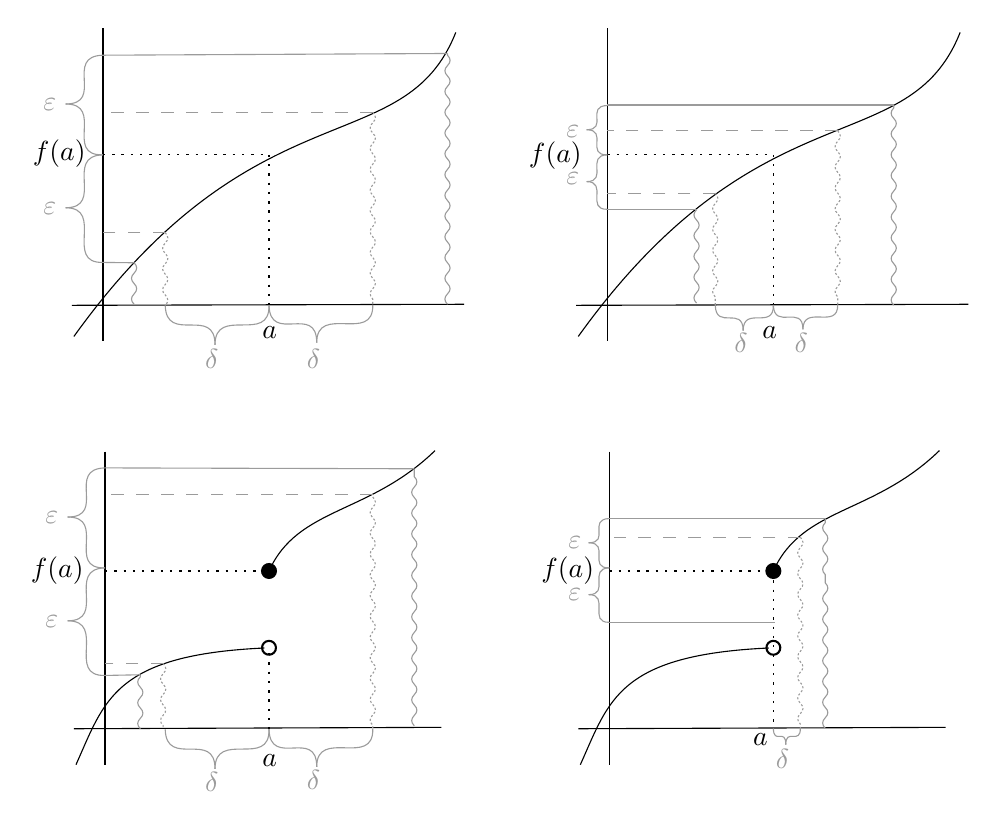
\begin{tikzpicture}[x=0.75pt,y=0.75pt,yscale=-1,xscale=1]
%uncomment if require: \path (0,428); %set diagram left start at 0, and has height of 428

%Straight Lines [id:da2730924968926851]
\draw    (71,155) -- (260,154.5) ;
%Straight Lines [id:da38663844155403493]
\draw    (86,21.5) -- (86,172.33) ;
%Curve Lines [id:da5832897062677318]
\draw    (72,170) .. controls (160,47.5) and (231,86.5) .. (256,23.5) ;
%Curve Lines [id:da15926967534570857]
\draw    (73,376.33) .. controls (86.86,345.64) and (90.92,323.45) .. (163.77,320.1) ;
\draw [shift={(166,320)}, rotate = 357.71] [color={rgb, 255:red, 0; green, 0; blue, 0 }  ][line width=0.75]      (0, 0) circle [x radius= 3.35, y radius= 3.35]   ;
%Curve Lines [id:da573129079856388]
\draw    (166,283) .. controls (180,252) and (214,256) .. (246,225) ;
\draw [shift={(166,283)}, rotate = 294.3] [color={rgb, 255:red, 0; green, 0; blue, 0 }  ][fill={rgb, 255:red, 0; green, 0; blue, 0 }  ][line width=0.75]      (0, 0) circle [x radius= 3.35, y radius= 3.35]   ;
%Straight Lines [id:da06544192635535961]
\draw  [dash pattern={on 0.84pt off 2.51pt}]  (166,82.5) -- (166,154.92) ;
%Straight Lines [id:da8462520068785757]
\draw  [dash pattern={on 0.84pt off 2.51pt}]  (86,82.5) -- (166,82.5) ;
%Straight Lines [id:da8033956316212987]
\draw [color={rgb, 255:red, 155; green, 155; blue, 155 }  ,draw opacity=1 ]   (86,34.5) -- (252,33.67) ;
%Straight Lines [id:da9058328806059841]
\draw [color={rgb, 255:red, 155; green, 155; blue, 155 }  ,draw opacity=1 ]   (86,134.33) -- (101,134.5) ;
%Straight Lines [id:da7683874289412185]
\draw    (72,359) -- (249,358.33) ;
%Straight Lines [id:da21021021460529377]
\draw    (87,225.5) -- (87,376.33) ;
%Straight Lines [id:da5263630709862186]
\draw  [dash pattern={on 0.84pt off 2.51pt}]  (166,322.58) -- (166,359.25) ;
%Straight Lines [id:da2255352189878881]
\draw  [dash pattern={on 0.84pt off 2.51pt}]  (87,283) -- (166,283) ;
%Straight Lines [id:da12241776303117424]
\draw [color={rgb, 255:red, 155; green, 155; blue, 155 }  ,draw opacity=1 ]   (87,233.33) -- (236,233.75) ;
%Straight Lines [id:da6551551228954233]
\draw [color={rgb, 255:red, 155; green, 155; blue, 155 }  ,draw opacity=1 ]   (87,333.33) -- (104,333) ;
%Straight Lines [id:da3470258564776276]
\draw [color={rgb, 255:red, 155; green, 155; blue, 155 }  ,draw opacity=1 ] [dash pattern={on 0.75pt off 0.75pt}]  (116,120) .. controls (117.67,121.67) and (117.67,123.33) .. (116,125) .. controls (114.33,126.67) and (114.33,128.33) .. (116,130) .. controls (117.67,131.67) and (117.67,133.33) .. (116,135) .. controls (114.33,136.67) and (114.33,138.33) .. (116,140) .. controls (117.67,141.67) and (117.67,143.33) .. (116,145) .. controls (114.33,146.67) and (114.33,148.33) .. (116,150) .. controls (117.67,151.67) and (117.67,153.33) .. (116,155) -- (116,155) ;
%Straight Lines [id:da2371091562631653]
\draw [color={rgb, 255:red, 155; green, 155; blue, 155 }  ,draw opacity=1 ] [dash pattern={on 0.75pt off 0.75pt}]  (216,62) .. controls (217.67,63.67) and (217.67,65.33) .. (216,67) .. controls (214.33,68.67) and (214.33,70.33) .. (216,72) .. controls (217.67,73.67) and (217.67,75.33) .. (216,77) .. controls (214.33,78.67) and (214.33,80.33) .. (216,82) .. controls (217.67,83.67) and (217.67,85.33) .. (216,87) .. controls (214.33,88.67) and (214.33,90.33) .. (216,92) .. controls (217.67,93.67) and (217.67,95.33) .. (216,97) .. controls (214.33,98.67) and (214.33,100.33) .. (216,102) .. controls (217.67,103.67) and (217.67,105.33) .. (216,107) .. controls (214.33,108.67) and (214.33,110.33) .. (216,112) .. controls (217.67,113.67) and (217.67,115.33) .. (216,117) .. controls (214.33,118.67) and (214.33,120.33) .. (216,122) .. controls (217.67,123.67) and (217.67,125.33) .. (216,127) .. controls (214.33,128.67) and (214.33,130.33) .. (216,132) .. controls (217.67,133.67) and (217.67,135.33) .. (216,137) .. controls (214.33,138.67) and (214.33,140.33) .. (216,142) .. controls (217.67,143.67) and (217.67,145.33) .. (216,147) .. controls (214.33,148.67) and (214.33,150.33) .. (216,152) -- (216,154.71) -- (216,154.71) ;
%Straight Lines [id:da47940446384008517]
\draw [color={rgb, 255:red, 155; green, 155; blue, 155 }  ,draw opacity=1 ] [dash pattern={on 4.5pt off 4.5pt}]  (116,120) -- (86,120) ;
%Straight Lines [id:da2718218581855085]
\draw [color={rgb, 255:red, 155; green, 155; blue, 155 }  ,draw opacity=1 ] [dash pattern={on 4.5pt off 4.5pt}]  (216,62) -- (86,62) ;
%Curve Lines [id:da7867325499156288]
\draw [color={rgb, 255:red, 155; green, 155; blue, 155 }  ,draw opacity=1 ]   (68,58) .. controls (87,58) and (67,35) .. (86,34.5) ;
%Curve Lines [id:da8389021578247982]
\draw [color={rgb, 255:red, 155; green, 155; blue, 155 }  ,draw opacity=1 ]   (68,58) .. controls (87,58) and (67,83) .. (86,82.5) ;
%Curve Lines [id:da6940267896547274]
\draw [color={rgb, 255:red, 155; green, 155; blue, 155 }  ,draw opacity=1 ]   (68,108) .. controls (87,108) and (67,83) .. (86,82.5) ;
%Curve Lines [id:da9368251006708403]
\draw [color={rgb, 255:red, 155; green, 155; blue, 155 }  ,draw opacity=1 ]   (68,108) .. controls (87,108) and (67,134.83) .. (86,134.33) ;
%Curve Lines [id:da7416463958304471]
\draw [color={rgb, 255:red, 155; green, 155; blue, 155 }  ,draw opacity=1 ]   (139.99,174) .. controls (140,155) and (116.5,174) .. (116,155) ;
%Curve Lines [id:da0946019041451891]
\draw [color={rgb, 255:red, 155; green, 155; blue, 155 }  ,draw opacity=1 ]   (139.99,174) .. controls (140,155) and (166.5,173.92) .. (166,154.92) ;
%Curve Lines [id:da8479225025412045]
\draw [color={rgb, 255:red, 155; green, 155; blue, 155 }  ,draw opacity=1 ]   (188.99,173) .. controls (189,154) and (166.5,173.92) .. (166,154.92) ;
%Curve Lines [id:da5287374586288269]
\draw [color={rgb, 255:red, 155; green, 155; blue, 155 }  ,draw opacity=1 ]   (188.99,173) .. controls (189,154) and (216.5,173.71) .. (216,154.71) ;
%Straight Lines [id:da5763369512697336]
\draw [color={rgb, 255:red, 155; green, 155; blue, 155 }  ,draw opacity=1 ]   (101,154.5) .. controls (99.33,152.83) and (99.33,151.17) .. (101,149.5) .. controls (102.67,147.83) and (102.67,146.17) .. (101,144.5) .. controls (99.33,142.83) and (99.33,141.17) .. (101,139.5) .. controls (102.67,137.83) and (102.67,136.17) .. (101,134.5) -- (101,134.5) ;
%Straight Lines [id:da9925497456851824]
\draw [color={rgb, 255:red, 155; green, 155; blue, 155 }  ,draw opacity=1 ]   (252,154.5) .. controls (250.33,152.83) and (250.33,151.17) .. (252,149.5) .. controls (253.67,147.83) and (253.67,146.17) .. (252,144.5) .. controls (250.33,142.83) and (250.33,141.17) .. (252,139.5) .. controls (253.67,137.83) and (253.67,136.17) .. (252,134.5) .. controls (250.33,132.83) and (250.33,131.17) .. (252,129.5) .. controls (253.67,127.83) and (253.67,126.17) .. (252,124.5) .. controls (250.33,122.83) and (250.33,121.17) .. (252,119.5) .. controls (253.67,117.83) and (253.67,116.17) .. (252,114.5) .. controls (250.33,112.83) and (250.33,111.17) .. (252,109.5) .. controls (253.67,107.83) and (253.67,106.17) .. (252,104.5) .. controls (250.33,102.83) and (250.33,101.17) .. (252,99.5) .. controls (253.67,97.83) and (253.67,96.17) .. (252,94.5) .. controls (250.33,92.83) and (250.33,91.17) .. (252,89.5) .. controls (253.67,87.83) and (253.67,86.17) .. (252,84.5) .. controls (250.33,82.83) and (250.33,81.17) .. (252,79.5) .. controls (253.67,77.83) and (253.67,76.17) .. (252,74.5) .. controls (250.33,72.83) and (250.33,71.17) .. (252,69.5) .. controls (253.67,67.83) and (253.67,66.17) .. (252,64.5) .. controls (250.33,62.83) and (250.33,61.17) .. (252,59.5) .. controls (253.67,57.83) and (253.67,56.17) .. (252,54.5) .. controls (250.33,52.83) and (250.33,51.17) .. (252,49.5) .. controls (253.67,47.83) and (253.67,46.17) .. (252,44.5) .. controls (250.33,42.83) and (250.33,41.17) .. (252,39.5) .. controls (253.67,37.83) and (253.67,36.17) .. (252,34.5) -- (252,33.67) -- (252,33.67) ;
%Curve Lines [id:da7131476230234577]
\draw [color={rgb, 255:red, 155; green, 155; blue, 155 }  ,draw opacity=1 ]   (69,257) .. controls (88,257) and (68,233.83) .. (87,233.33) ;
%Curve Lines [id:da5212410455410692]
\draw [color={rgb, 255:red, 155; green, 155; blue, 155 }  ,draw opacity=1 ]   (69,257) .. controls (88,257) and (68,282) .. (87,281.5) ;
%Curve Lines [id:da8037674418363849]
\draw [color={rgb, 255:red, 155; green, 155; blue, 155 }  ,draw opacity=1 ]   (69,307) .. controls (88,307) and (68,282) .. (87,281.5) ;
%Curve Lines [id:da3061502012065347]
\draw [color={rgb, 255:red, 155; green, 155; blue, 155 }  ,draw opacity=1 ]   (69,307) .. controls (88,307) and (68,333.83) .. (87,333.33) ;
%Curve Lines [id:da838846723146208]
\draw [color={rgb, 255:red, 155; green, 155; blue, 155 }  ,draw opacity=1 ]   (139.99,378.34) .. controls (140,359.34) and (116.5,378.33) .. (116,359.33) ;
%Curve Lines [id:da45926415056497105]
\draw [color={rgb, 255:red, 155; green, 155; blue, 155 }  ,draw opacity=1 ]   (139.99,378.34) .. controls (140,359.34) and (166.5,378.25) .. (166,359.25) ;
%Curve Lines [id:da1812164249288335]
\draw [color={rgb, 255:red, 155; green, 155; blue, 155 }  ,draw opacity=1 ]   (188.99,377.34) .. controls (189,358.34) and (166.5,378.25) .. (166,359.25) ;
%Curve Lines [id:da5310165714599331]
\draw [color={rgb, 255:red, 155; green, 155; blue, 155 }  ,draw opacity=1 ]   (188.99,377.34) .. controls (189,358.34) and (216.5,378.04) .. (216,359.04) ;
%Straight Lines [id:da1373743464903565]
\draw [color={rgb, 255:red, 155; green, 155; blue, 155 }  ,draw opacity=1 ] [dash pattern={on 0.75pt off 0.75pt}]  (115,327.5) .. controls (116.67,329.17) and (116.67,330.83) .. (115,332.5) .. controls (113.33,334.17) and (113.33,335.83) .. (115,337.5) .. controls (116.67,339.17) and (116.67,340.83) .. (115,342.5) .. controls (113.33,344.17) and (113.33,345.83) .. (115,347.5) .. controls (116.67,349.17) and (116.67,350.83) .. (115,352.5) .. controls (113.33,354.17) and (113.33,355.83) .. (115,357.5) -- (115,359) -- (115,359) ;
%Straight Lines [id:da30273639101181327]
\draw [color={rgb, 255:red, 155; green, 155; blue, 155 }  ,draw opacity=1 ] [dash pattern={on 0.75pt off 0.75pt}]  (216,247.33) .. controls (217.67,249) and (217.67,250.66) .. (216,252.33) .. controls (214.33,254) and (214.33,255.66) .. (216,257.33) .. controls (217.67,259) and (217.67,260.66) .. (216,262.33) .. controls (214.33,264) and (214.33,265.66) .. (216,267.33) .. controls (217.67,269) and (217.67,270.66) .. (216,272.33) .. controls (214.33,274) and (214.33,275.66) .. (216,277.33) .. controls (217.67,279) and (217.67,280.66) .. (216,282.33) .. controls (214.33,284) and (214.33,285.66) .. (216,287.33) .. controls (217.67,289) and (217.67,290.66) .. (216,292.33) .. controls (214.33,294) and (214.33,295.66) .. (216,297.33) .. controls (217.67,299) and (217.67,300.66) .. (216,302.33) .. controls (214.33,304) and (214.33,305.66) .. (216,307.33) .. controls (217.67,309) and (217.67,310.66) .. (216,312.33) .. controls (214.33,314) and (214.33,315.66) .. (216,317.33) .. controls (217.67,319) and (217.67,320.66) .. (216,322.33) .. controls (214.33,324) and (214.33,325.66) .. (216,327.33) .. controls (217.67,329) and (217.67,330.66) .. (216,332.33) .. controls (214.33,334) and (214.33,335.66) .. (216,337.33) .. controls (217.67,339) and (217.67,340.66) .. (216,342.33) .. controls (214.33,344) and (214.33,345.66) .. (216,347.33) .. controls (217.67,349) and (217.67,350.66) .. (216,352.33) .. controls (214.33,354) and (214.33,355.66) .. (216,357.33) -- (216,359.04) -- (216,359.04) ;
%Straight Lines [id:da6690760580285089]
\draw [color={rgb, 255:red, 155; green, 155; blue, 155 }  ,draw opacity=1 ] [dash pattern={on 4.5pt off 4.5pt}]  (115,327.5) -- (87,327.5) ;
%Straight Lines [id:da023392902319420816]
\draw [color={rgb, 255:red, 155; green, 155; blue, 155 }  ,draw opacity=1 ] [dash pattern={on 4.5pt off 4.5pt}]  (216,246) -- (87,246) ;
%Straight Lines [id:da7002803226646901]
\draw [color={rgb, 255:red, 155; green, 155; blue, 155 }  ,draw opacity=1 ]   (104,359) .. controls (102.33,357.33) and (102.33,355.67) .. (104,354) .. controls (105.67,352.33) and (105.67,350.67) .. (104,349) .. controls (102.33,347.33) and (102.33,345.67) .. (104,344) .. controls (105.67,342.33) and (105.67,340.67) .. (104,339) .. controls (102.33,337.33) and (102.33,335.67) .. (104,334) -- (104,333) -- (104,333) ;
%Straight Lines [id:da5440309336359443]
\draw [color={rgb, 255:red, 155; green, 155; blue, 155 }  ,draw opacity=1 ]   (236,357.58) .. controls (234.33,355.91) and (234.33,354.25) .. (236,352.58) .. controls (237.67,350.91) and (237.67,349.25) .. (236,347.58) .. controls (234.33,345.91) and (234.33,344.25) .. (236,342.58) .. controls (237.67,340.91) and (237.67,339.25) .. (236,337.58) .. controls (234.33,335.91) and (234.33,334.25) .. (236,332.58) .. controls (237.67,330.91) and (237.67,329.25) .. (236,327.58) .. controls (234.33,325.91) and (234.33,324.25) .. (236,322.58) .. controls (237.67,320.91) and (237.67,319.25) .. (236,317.58) .. controls (234.33,315.91) and (234.33,314.25) .. (236,312.58) .. controls (237.67,310.91) and (237.67,309.25) .. (236,307.58) .. controls (234.33,305.91) and (234.33,304.25) .. (236,302.58) .. controls (237.67,300.91) and (237.67,299.25) .. (236,297.58) .. controls (234.33,295.91) and (234.33,294.25) .. (236,292.58) .. controls (237.67,290.91) and (237.67,289.25) .. (236,287.58) .. controls (234.33,285.91) and (234.33,284.25) .. (236,282.58) .. controls (237.67,280.91) and (237.67,279.25) .. (236,277.58) .. controls (234.33,275.91) and (234.33,274.25) .. (236,272.58) .. controls (237.67,270.91) and (237.67,269.25) .. (236,267.58) .. controls (234.33,265.91) and (234.33,264.25) .. (236,262.58) .. controls (237.67,260.91) and (237.67,259.25) .. (236,257.58) .. controls (234.33,255.91) and (234.33,254.25) .. (236,252.58) .. controls (237.67,250.91) and (237.67,249.25) .. (236,247.58) .. controls (234.33,245.91) and (234.33,244.25) .. (236,242.58) .. controls (237.67,240.91) and (237.67,239.25) .. (236,237.58) -- (236,233.75) -- (236,233.75) ;

%Straight Lines [id:da8513462018635212]
\draw    (314,155) -- (503,154.5) ;
%Straight Lines [id:da27501056686778513]
\draw    (329,21.5) -- (329,172.33) ;
%Curve Lines [id:da5516996470591613]
\draw    (315,170) .. controls (403,47.5) and (474,86.5) .. (499,23.5) ;
%Curve Lines [id:da2905586367584121]
\draw    (316,376.33) .. controls (329.86,345.64) and (333.92,323.45) .. (406.77,320.1) ;
\draw [shift={(409,320)}, rotate = 357.71] [color={rgb, 255:red, 0; green, 0; blue, 0 }  ][line width=0.75]      (0, 0) circle [x radius= 3.35, y radius= 3.35]   ;
%Curve Lines [id:da17327963328411955]
\draw    (409,283) .. controls (423,252) and (457,256) .. (489,225) ;
\draw [shift={(409,283)}, rotate = 294.3] [color={rgb, 255:red, 0; green, 0; blue, 0 }  ][fill={rgb, 255:red, 0; green, 0; blue, 0 }  ][line width=0.75]      (0, 0) circle [x radius= 3.35, y radius= 3.35]   ;
%Straight Lines [id:da4442118515906792]
\draw  [dash pattern={on 0.84pt off 2.51pt}]  (409,82.5) -- (409,154.92) ;
%Straight Lines [id:da4615400041448172]
\draw  [dash pattern={on 0.84pt off 2.51pt}]  (329,82.5) -- (409,82.5) ;
%Straight Lines [id:da9140897903442382]
\draw [color={rgb, 255:red, 155; green, 155; blue, 155 }  ,draw opacity=1 ]   (329,58.5) -- (467,58.5) ;
%Straight Lines [id:da8879320022705979]
\draw [color={rgb, 255:red, 155; green, 155; blue, 155 }  ,draw opacity=1 ]   (329,108.73) -- (372,108.73) ;
%Straight Lines [id:da17895890987358554]
\draw    (315,359) -- (492,358.33) ;
%Straight Lines [id:da05857321637633417]
\draw    (330,225.5) -- (330,376.33) ;
%Straight Lines [id:da07307770178123163]
\draw  [dash pattern={on 0.84pt off 2.51pt}]  (409,283) -- (409,359.25) ;
%Straight Lines [id:da06234038795466201]
\draw  [dash pattern={on 0.84pt off 2.51pt}]  (330,283) -- (409,283) ;
%Straight Lines [id:da8599377579018705]
\draw [color={rgb, 255:red, 155; green, 155; blue, 155 }  ,draw opacity=1 ]   (330,257.73) -- (434,257.73) ;
%Straight Lines [id:da9417232436931344]
\draw [color={rgb, 255:red, 155; green, 155; blue, 155 }  ,draw opacity=1 ]   (330,307.73) -- (410,307.73) ;
%Straight Lines [id:da21280146915905584]
\draw [color={rgb, 255:red, 155; green, 155; blue, 155 }  ,draw opacity=1 ] [dash pattern={on 0.75pt off 0.75pt}]  (381,100.93) .. controls (382.67,102.6) and (382.67,104.26) .. (381,105.93) .. controls (379.33,107.6) and (379.33,109.26) .. (381,110.93) .. controls (382.67,112.6) and (382.67,114.26) .. (381,115.93) .. controls (379.33,117.6) and (379.33,119.26) .. (381,120.93) .. controls (382.67,122.6) and (382.67,124.26) .. (381,125.93) .. controls (379.33,127.6) and (379.33,129.26) .. (381,130.93) .. controls (382.67,132.6) and (382.67,134.26) .. (381,135.93) .. controls (379.33,137.6) and (379.33,139.26) .. (381,140.93) .. controls (382.67,142.6) and (382.67,144.26) .. (381,145.93) .. controls (379.33,147.6) and (379.33,149.26) .. (381,150.93) -- (381,154.9) -- (381,154.9) ;
%Straight Lines [id:da1757874388402605]
\draw [color={rgb, 255:red, 155; green, 155; blue, 155 }  ,draw opacity=1 ] [dash pattern={on 0.75pt off 0.75pt}]  (440,70.93) .. controls (441.67,72.6) and (441.67,74.26) .. (440,75.93) .. controls (438.33,77.6) and (438.33,79.26) .. (440,80.93) .. controls (441.67,82.6) and (441.67,84.26) .. (440,85.93) .. controls (438.33,87.6) and (438.33,89.26) .. (440,90.93) .. controls (441.67,92.6) and (441.67,94.26) .. (440,95.93) .. controls (438.33,97.6) and (438.33,99.26) .. (440,100.93) .. controls (441.67,102.6) and (441.67,104.26) .. (440,105.93) .. controls (438.33,107.6) and (438.33,109.26) .. (440,110.93) .. controls (441.67,112.6) and (441.67,114.26) .. (440,115.93) .. controls (438.33,117.6) and (438.33,119.26) .. (440,120.93) .. controls (441.67,122.6) and (441.67,124.26) .. (440,125.93) .. controls (438.33,127.6) and (438.33,129.26) .. (440,130.93) .. controls (441.67,132.6) and (441.67,134.26) .. (440,135.93) .. controls (438.33,137.6) and (438.33,139.26) .. (440,140.93) .. controls (441.67,142.6) and (441.67,144.26) .. (440,145.93) .. controls (438.33,147.6) and (438.33,149.26) .. (440,150.93) -- (440,154.71) -- (440,154.71) ;
%Straight Lines [id:da4275079323186526]
\draw [color={rgb, 255:red, 155; green, 155; blue, 155 }  ,draw opacity=1 ] [dash pattern={on 4.5pt off 4.5pt}]  (381,100.93) -- (329,100.93) ;
%Straight Lines [id:da4596336138709165]
\draw [color={rgb, 255:red, 155; green, 155; blue, 155 }  ,draw opacity=1 ] [dash pattern={on 4.5pt off 4.5pt}]  (440,70.93) -- (329,70.93) ;
%Curve Lines [id:da6338318263176852]
\draw [color={rgb, 255:red, 155; green, 155; blue, 155 }  ,draw opacity=1 ]   (394.44,167.24) .. controls (394.44,154.9) and (381.28,167.24) .. (381,154.9) ;
%Curve Lines [id:da34761840807493516]
\draw [color={rgb, 255:red, 155; green, 155; blue, 155 }  ,draw opacity=1 ]   (394.44,167.24) .. controls (394.44,154.9) and (409.28,167.19) .. (409,154.84) ;
%Curve Lines [id:da25995298856914184]
\draw [color={rgb, 255:red, 155; green, 155; blue, 155 }  ,draw opacity=1 ]   (423.25,166.59) .. controls (423.26,154.25) and (409.31,167.19) .. (409,154.84) ;
%Curve Lines [id:da7818991925364918]
\draw [color={rgb, 255:red, 155; green, 155; blue, 155 }  ,draw opacity=1 ]   (423.25,166.59) .. controls (423.26,154.25) and (440.3,167.05) .. (440,154.71) ;
%Straight Lines [id:da007122223942663375]
\draw [color={rgb, 255:red, 155; green, 155; blue, 155 }  ,draw opacity=1 ]   (372,153.93) .. controls (370.33,152.26) and (370.33,150.6) .. (372,148.93) .. controls (373.67,147.26) and (373.67,145.6) .. (372,143.93) .. controls (370.33,142.26) and (370.33,140.6) .. (372,138.93) .. controls (373.67,137.26) and (373.67,135.6) .. (372,133.93) .. controls (370.33,132.26) and (370.33,130.6) .. (372,128.93) .. controls (373.67,127.26) and (373.67,125.6) .. (372,123.93) .. controls (370.33,122.26) and (370.33,120.6) .. (372,118.93) .. controls (373.67,117.26) and (373.67,115.6) .. (372,113.93) .. controls (370.33,112.26) and (370.33,110.6) .. (372,108.93) -- (372,108.73) -- (372,108.73) ;
%Straight Lines [id:da2226129700521089]
\draw [color={rgb, 255:red, 155; green, 155; blue, 155 }  ,draw opacity=1 ]   (467,154.93) .. controls (465.33,153.26) and (465.33,151.6) .. (467,149.93) .. controls (468.67,148.26) and (468.67,146.6) .. (467,144.93) .. controls (465.33,143.26) and (465.33,141.6) .. (467,139.93) .. controls (468.67,138.26) and (468.67,136.6) .. (467,134.93) .. controls (465.33,133.26) and (465.33,131.6) .. (467,129.93) .. controls (468.67,128.26) and (468.67,126.6) .. (467,124.93) .. controls (465.33,123.26) and (465.33,121.6) .. (467,119.93) .. controls (468.67,118.26) and (468.67,116.6) .. (467,114.93) .. controls (465.33,113.26) and (465.33,111.6) .. (467,109.93) .. controls (468.67,108.26) and (468.67,106.6) .. (467,104.93) .. controls (465.33,103.26) and (465.33,101.6) .. (467,99.93) .. controls (468.67,98.26) and (468.67,96.6) .. (467,94.93) .. controls (465.33,93.26) and (465.33,91.6) .. (467,89.93) .. controls (468.67,88.26) and (468.67,86.6) .. (467,84.93) .. controls (465.33,83.26) and (465.33,81.6) .. (467,79.93) .. controls (468.67,78.26) and (468.67,76.6) .. (467,74.93) .. controls (465.33,73.26) and (465.33,71.6) .. (467,69.93) .. controls (468.67,68.26) and (468.67,66.6) .. (467,64.93) .. controls (465.33,63.26) and (465.33,61.6) .. (467,59.93) -- (467,58.5) -- (467,58.5) ;
%Curve Lines [id:da698734706179845]
\draw [color={rgb, 255:red, 155; green, 155; blue, 155 }  ,draw opacity=1 ]   (320,269.41) .. controls (330.56,269.41) and (319.44,257.98) .. (330,257.73) ;
%Curve Lines [id:da5504971774940504]
\draw [color={rgb, 255:red, 155; green, 155; blue, 155 }  ,draw opacity=1 ]   (320,269.41) .. controls (330.56,269.41) and (319.44,281.75) .. (330,281.5) ;
%Curve Lines [id:da665922234047422]
\draw [color={rgb, 255:red, 155; green, 155; blue, 155 }  ,draw opacity=1 ]   (320,294.4) .. controls (330.56,294.4) and (319.44,281.75) .. (330,281.5) ;
%Curve Lines [id:da7956304462768429]
\draw [color={rgb, 255:red, 155; green, 155; blue, 155 }  ,draw opacity=1 ]   (320,294.4) .. controls (330.56,294.4) and (319.44,307.98) .. (330,307.73) ;
%Straight Lines [id:da7224291382128996]
\draw [color={rgb, 255:red, 155; green, 155; blue, 155 }  ,draw opacity=1 ] [dash pattern={on 0.75pt off 0.75pt}]  (422,266.73) .. controls (423.67,268.4) and (423.67,270.06) .. (422,271.73) .. controls (420.33,273.4) and (420.33,275.06) .. (422,276.73) .. controls (423.67,278.4) and (423.67,280.06) .. (422,281.73) .. controls (420.33,283.4) and (420.33,285.06) .. (422,286.73) .. controls (423.67,288.4) and (423.67,290.06) .. (422,291.73) .. controls (420.33,293.4) and (420.33,295.06) .. (422,296.73) .. controls (423.67,298.4) and (423.67,300.06) .. (422,301.73) .. controls (420.33,303.4) and (420.33,305.06) .. (422,306.73) .. controls (423.67,308.4) and (423.67,310.06) .. (422,311.73) .. controls (420.33,313.4) and (420.33,315.06) .. (422,316.73) .. controls (423.67,318.4) and (423.67,320.06) .. (422,321.73) .. controls (420.33,323.4) and (420.33,325.06) .. (422,326.73) .. controls (423.67,328.4) and (423.67,330.06) .. (422,331.73) .. controls (420.33,333.4) and (420.33,335.06) .. (422,336.73) .. controls (423.67,338.4) and (423.67,340.06) .. (422,341.73) .. controls (420.33,343.4) and (420.33,345.06) .. (422,346.73) .. controls (423.67,348.4) and (423.67,350.06) .. (422,351.73) .. controls (420.33,353.4) and (420.33,355.06) .. (422,356.73) -- (422,358.73) -- (422,358.73) ;
%Straight Lines [id:da4206208106816536]
\draw [color={rgb, 255:red, 155; green, 155; blue, 155 }  ,draw opacity=1 ] [dash pattern={on 4.5pt off 4.5pt}]  (422,266.73) -- (330,266.73) ;
%Straight Lines [id:da909571198522956]
\draw [color={rgb, 255:red, 155; green, 155; blue, 155 }  ,draw opacity=1 ]   (434,358.73) .. controls (432.33,357.06) and (432.33,355.4) .. (434,353.73) .. controls (435.67,352.06) and (435.67,350.4) .. (434,348.73) .. controls (432.33,347.06) and (432.33,345.4) .. (434,343.73) .. controls (435.67,342.06) and (435.67,340.4) .. (434,338.73) .. controls (432.33,337.06) and (432.33,335.4) .. (434,333.73) .. controls (435.67,332.06) and (435.67,330.4) .. (434,328.73) .. controls (432.33,327.06) and (432.33,325.4) .. (434,323.73) .. controls (435.67,322.06) and (435.67,320.4) .. (434,318.73) .. controls (432.33,317.06) and (432.33,315.4) .. (434,313.73) .. controls (435.67,312.06) and (435.67,310.4) .. (434,308.73) .. controls (432.33,307.06) and (432.33,305.4) .. (434,303.73) .. controls (435.67,302.06) and (435.67,300.4) .. (434,298.73) .. controls (432.33,297.06) and (432.33,295.4) .. (434,293.73) .. controls (435.67,292.06) and (435.67,290.4) .. (434,288.73) -- (434,284.73) -- (434,284.73) .. controls (432.33,283.06) and (432.33,281.4) .. (434,279.73) .. controls (435.67,278.06) and (435.67,276.4) .. (434,274.73) .. controls (432.33,273.06) and (432.33,271.4) .. (434,269.73) .. controls (435.67,268.06) and (435.67,266.4) .. (434,264.73) .. controls (432.33,263.06) and (432.33,261.4) .. (434,259.73) -- (434,257.73) -- (434,257.73) ;
%Curve Lines [id:da9457581571351961]
\draw [color={rgb, 255:red, 155; green, 155; blue, 155 }  ,draw opacity=1 ]   (319,70.41) .. controls (329.56,70.41) and (318.44,58.98) .. (329,58.73) ;
%Curve Lines [id:da3811228849623747]
\draw [color={rgb, 255:red, 155; green, 155; blue, 155 }  ,draw opacity=1 ]   (319,70.41) .. controls (329.56,70.41) and (318.44,82.75) .. (329,82.5) ;
%Curve Lines [id:da45732723484863413]
\draw [color={rgb, 255:red, 155; green, 155; blue, 155 }  ,draw opacity=1 ]   (319,95.4) .. controls (329.56,95.4) and (318.44,82.75) .. (329,82.5) ;
%Curve Lines [id:da6190962246605269]
\draw [color={rgb, 255:red, 155; green, 155; blue, 155 }  ,draw opacity=1 ]   (319,95.4) .. controls (329.56,95.4) and (318.44,108.98) .. (329,108.73) ;
%Curve Lines [id:da05897663741609804]
\draw [color={rgb, 255:red, 155; green, 155; blue, 155 }  ,draw opacity=1 ]   (414.98,366.62) .. controls (414.98,358.4) and (409.13,367.01) .. (409,358.8) ;
%Curve Lines [id:da23661597723290972]
\draw [color={rgb, 255:red, 155; green, 155; blue, 155 }  ,draw opacity=1 ]   (414.98,366.62) .. controls (414.98,358.4) and (422.13,366.92) .. (422,358.71) ;


% Text Node
\draw (56,54) node [anchor=north west][inner sep=0.75pt]  [color={rgb, 255:red, 155; green, 155; blue, 155 }  ,opacity=1 ]  {$\varepsilon $};
% Text Node
\draw (56,104) node [anchor=north west][inner sep=0.75pt]  [color={rgb, 255:red, 155; green, 155; blue, 155 }  ,opacity=1 ]  {$\varepsilon $};
% Text Node
\draw (134,175) node [anchor=north west][inner sep=0.75pt]  [color={rgb, 255:red, 155; green, 155; blue, 155 }  ,opacity=1 ]  {$\delta $};
% Text Node
\draw (183,175) node [anchor=north west][inner sep=0.75pt]  [color={rgb, 255:red, 155; green, 155; blue, 155 }  ,opacity=1 ]  {$\delta $};
% Text Node
\draw (161.5,164) node [anchor=north west][inner sep=0.75pt]    {$a$};
% Text Node
\draw (51,74) node [anchor=north west][inner sep=0.75pt]    {$f( a)$};



% Text Node
\draw (57,253) node [anchor=north west][inner sep=0.75pt]  [color={rgb, 255:red, 155; green, 155; blue, 155 }  ,opacity=1 ]  {$\varepsilon $};
% Text Node
\draw (57,303) node [anchor=north west][inner sep=0.75pt]  [color={rgb, 255:red, 155; green, 155; blue, 155 }  ,opacity=1 ]  {$\varepsilon $};
% Text Node
\draw (50,275) node [anchor=north west][inner sep=0.75pt]    {$f( a)$};
% Text Node
\draw (134,378.73) node [anchor=north west][inner sep=0.75pt]  [color={rgb, 255:red, 155; green, 155; blue, 155 }  ,opacity=1 ]  {$\delta $};
% Text Node
\draw (183,377.73) node [anchor=north west][inner sep=0.75pt]  [color={rgb, 255:red, 155; green, 155; blue, 155 }  ,opacity=1 ]  {$\delta $};
% Text Node
\draw (161.5,370) node [anchor=north west][inner sep=0.75pt]    {$a$};



% Text Node
\draw (389,167) node [anchor=north west][inner sep=0.75pt]  [color={rgb, 255:red, 155; green, 155; blue, 155 }  ,opacity=1 ]  {$\delta $};
% Text Node
\draw (418,167) node [anchor=north west][inner sep=0.75pt]  [color={rgb, 255:red, 155; green, 155; blue, 155 }  ,opacity=1 ]  {$\delta $};
% Text Node
\draw (402.5,164) node [anchor=north west][inner sep=0.75pt]    {$a$};
% Text Node
\draw (308,67) node [anchor=north west][inner sep=0.75pt]  [color={rgb, 255:red, 155; green, 155; blue, 155 }  ,opacity=1 ]  {$\varepsilon $};
% Text Node
\draw (308,90) node [anchor=north west][inner sep=0.75pt]  [color={rgb, 255:red, 155; green, 155; blue, 155 }  ,opacity=1 ]  {$\varepsilon $};
% Text Node
\draw (290,75) node [anchor=north west][inner sep=0.75pt]    {$f( a)$};


% Text Node
\draw (296,275) node [anchor=north west][inner sep=0.75pt]    {$f(a)$};
% Text Node
\draw (398,360) node [anchor=north west][inner sep=0.75pt]    {$a$};
% Text Node
\draw (309,265) node [anchor=north west][inner sep=0.75pt]  [color={rgb, 255:red, 155; green, 155; blue, 155 }  ,opacity=1 ]  {$\varepsilon $};
% Text Node
\draw (309,290) node [anchor=north west][inner sep=0.75pt]  [color={rgb, 255:red, 155; green, 155; blue, 155 }  ,opacity=1 ]  {$\varepsilon $};
% Text Node
\draw (409,367.65) node [anchor=north west][inner sep=0.75pt]  [color={rgb, 255:red, 155; green, 155; blue, 155 }  ,opacity=1 ]  {$\delta $};


\end{tikzpicture}
}
\caption{A cartoon of the $\varepsilon-\delta$ definition of a limit}
\label{epsilon-cartoon}
\end{figure}

Figure \ref{epsilon-cartoon} is the classic picture you should try to commit to memory, or at very least, thoroughly understand. Here is how you should think about it:
\begin{enumerate}
\item Let $\varepsilon$ define an interval around $f(a)$ on the $y$-axis.
\item Then trace the interval right until it hits the graph of the function (solid gray line), and wherever the solid gray line meets the function, draw the solid squiggly line down to meet the $x$-axis.
\item Choose $\delta$ small enough so that when the reverse action is done (trace the $\delta$ interval up with the dotted squiggly line to the function and then left with the dashed line to the $y$-axis), the resulting interval is contained within the $\varepsilon$ interval.
\end{enumerate}

While the function graphed in the top two plots has a limit at $a$, the function that is graphed in the bottom two plots does not. For this function the first value of $\varepsilon$ (graph on the left) is not small enough to detect the jump discontinuity, but on the second (graph on the right), the $\varepsilon$ given is so small that no value of $\delta$ can be big enough to ignore jump.

It may be helpful to think about the definition of a limit as a game/conversation between two people, Alex and Blake. Alex is trying to claim that the limit of $f$ as $x\to a$ is L, and Blake is doing their best job to contest it. Here is how their conversation might go:
\begin{itemize}
\item[A:] I think the limit of $f(x)=3x+1$ as $x$ approaches $2$ is 7.
\item[B:] Well if you think so, can you ensure that $|f(x)-7|<\frac{1}{10}$?
\item[A:] Yes! If we take $x$ such that $|x-2|<1/30$, then
$$|f(x)-7|=|3x + 1 - 7| = |3x-6| = 3|x-2| < 3(1/30) = 1/10.$$
\end{itemize}
In this example, $\varepsilon = 1/10$ and $\delta = 1/30$. However, if we want to really prove that the limit is 7, we let $\epsilon>0$ be arbitrary, and take $\delta = \varepsilon/3$. Then for any $x$ such that $|x-2|<\delta$,
$$|f(x)-7|=|3x + 1 - 7| = |3x-6| = 3|x-2| < 3(\varepsilon/3) = \varepsilon.$$

For simple examples, it is pretty easy to work backwards and figure out what $\delta$ should be, but for more complicated functions $f$, it can be more difficult. Here is a \href{https://www.desmos.com/calculator/cuoca85inx}{Desmos example} that shows dynamically how $\delta$ can depend on $\varepsilon$.


\subsection{Continuity}

Intuitively, a function is continuous if you can draw its graph without lifting up your pencil. We can use limits to write a more precise definition: a function $f$ is \textbf{continuous at $a$} if three conditions are satisfied:
\begin{enumerate}
\item[(a)] $f$ is defined at $a$ (i.e. $f(a)$ makes sense)
\item[(b)] $\displaystyle\lim_{x\to a^+} f(x)= f(a)$
\item[(c)] $\displaystyle\lim_{x\to a^-} f(x)= f(a)$
\end{enumerate}

In other words, a function is continuous at a point if its value and limit match at that point.

If $U$ is a subset of $\R$ and $f$ is continuous at every point in $U$, then we say that $f$ is \textbf{continuous on $U$}.

In the definition above, if (b) and/or (c) is not true (or one of the sided limits doesn't exist), then $f$ is \textbf{discontinuous at $a$}. Here are three types of discontinuities that you may encounter: if $f$ is discontinuous at $a$, then
\begin{enumerate}
\item $f$ has a \textbf{removable discontinuity} at $a$ if $\displaystyle\lim _{x \to a} f(x)$ exists and is a real number, (but $\displaystyle f(a)\neq\lim _{x \to a} f(x)$).
\item $f$ has a \textbf{jump discontinuity} at $a$ if $\displaystyle\lim _{x \to a^{-}} f(x)$ and $\displaystyle\lim _{x \to a^{+}} f(x)$ both exist and are real numbers, but are different.
\item $f$ has an \textbf{infinite discontinuity} at $a$ if $\displaystyle\lim _{x \to a^{-}} f(x)=\pm \infty$ or $\displaystyle\lim _{x \to a^{+}} f(x)=\pm \infty$.
\end{enumerate}
\mar{Draw a picture of each kind of discontinuity.}

Note that if $a$ is not in the domain of $f$, then $f$ is neither continuous or discontinuous at $a$.


\section{Properties of Limits}


\subsection{Limit Laws}

There are several \textit{limit laws} that will be useful for computing limits. They can all be proven using the $\varepsilon-\delta$ definition of the limit, but you can just believe them.

Suppose $\displaystyle\lim _{x \to a} f(x)=L$ and $\displaystyle\lim _{x \to a} g(x)=M$, let $c$ be a constant, and let $n$ be a positive integer.

\begin{center}
\def\arraystretch{2}
\begin{tabular}{@{}ll@{}}
\toprule[0.4mm]
\textbf{Constant Law} & $\displaystyle \lim_{x\to a} b= b$\\
\textbf{Identity Law} & $\displaystyle\lim_{x\to a}x = a$\\
\textbf{Sum law} & $\displaystyle\lim _{x \rightarrow a}(f(x)+g(x))=\lim _{x \rightarrow a} f(x)+\lim _{x \rightarrow a} g(x)=L+M$ \\
\textbf{Difference law} & $\displaystyle\lim _{x \rightarrow a}(f(x)-g(x))=\lim _{x \rightarrow a} f(x)-\lim _{x \rightarrow a} g(x)=L-M$ \\
\textbf{Constant Multiple law} & $\displaystyle\lim _{x \rightarrow a} c f(x)=c \cdot \lim _{x \rightarrow a} f(x)=c L$ \\
\textbf{Product law} & $\displaystyle\lim _{x \rightarrow a}(f(x) \cdot g(x))=\lim _{x \rightarrow a} f(x) \cdot \lim _{x \rightarrow a} g(x)=L \cdot M$ \\
\textbf{Quotient law} & $\displaystyle\lim _{x \rightarrow a} \frac{f(x)}{g(x)}=\frac{\displaystyle\lim _{x \rightarrow a} f(x)}{\displaystyle\lim _{x \rightarrow a} g(x)}=\frac{L}{M}$ for $M \neq 0$ \\
\textbf{Power law} & $\displaystyle\lim _{x \rightarrow a}(f(x))^{n}=\left(\lim _{x \rightarrow a} f(x)\right)^{n}=L^{n}$\\
\textbf{Root law} & $\displaystyle\lim _{x \rightarrow a} \sqrt[n]{f(x)}=\sqrt[n]{\lim _{x \rightarrow a} f(x)}=\sqrt[n]{L}$ for all $L$ if $n$ is odd,\\
& and for $L \geq 0$ if $n$ is even and $f(x) \geq 0 .$ \\
\bottomrule[0.4mm]
\end{tabular}
\end{center}
\mar{Write out what each limit law means in plain English.}


The first two laws should be obvious. 
The last two laws are special cases of the following theorem.

\begin{thm}[Composite Function Theorem]
If $f(x)$ is continuous at $L$ and $\displaystyle\lim _{x \to a} g(x)=L$, then
$$\lim _{x \to a} f(g(x))=f\left(\lim _{x \to a} g(x)\right)=f(L).$$
\end{thm}



\subsection{Using Continuity}

You should believe that the following types of functions are continuous at every point in their domains:
\begin{itemize}
\item polynomials
\item rational functions
\item trig and inverse trig functions
\item exponential functions
\item logarithms
\end{itemize}

An \textbf{algebraic combination of continuous functions} (ACCF) is a sum, product, exponentiation, or composition of continuous functions.

\begin{thm}
Any ACCF is continuous on its domain.
\end{thm}


To finish, another very useful theorem:

\begin{thm}[The Intermediate Value Theorem]
Let $f$ be continuous over a closed, bounded interval $[a, b]$. If $z$ is any real number between $f(a)$ and $f(b)$, then there is a number $c$ in $[a, b]$ satisfying $f(c)=z$.
\end{thm}

\begin{figure}[h!]
\centering
\fbox{
\tikzset{every picture/.style={line width=0.75pt}}
\begin{tikzpicture}[x=0.75pt,y=0.75pt,yscale=-1,xscale=1]
%uncomment if require: \path (0,374); %set diagram left start at 0, and has height of 374

%Straight Lines [id:da38498324007722995]
\draw    (159,287) -- (517,287.2) ;
%Straight Lines [id:da5792876353049934]
\draw    (180,98.33) -- (180,328.2) ;
%Curve Lines [id:da7286746857142028]
\draw    (180,287) .. controls (366,94) and (463,235.33) .. (496,98.33) ;
%Straight Lines [id:da23865898502362382]
\draw  [dash pattern={on 0.84pt off 2.51pt}]  (254,223.67) -- (254,288.2) ;
%Straight Lines [id:da15690973094077898]
\draw  [dash pattern={on 0.84pt off 2.51pt}]  (429,167.67) -- (429,287) ;
%Straight Lines [id:da0889210997343266]
\draw  [dash pattern={on 0.84pt off 2.51pt}]  (429,167.67) -- (179,167.67) ;
%Straight Lines [id:da7783842106309002]
\draw  [dash pattern={on 0.84pt off 2.51pt}]  (254,223.67) -- (181,223.67) ;
%Straight Lines [id:da6580337268340255]
\draw  [dash pattern={on 0.84pt off 2.51pt}]  (303,197.1) -- (180,197.1) ;
%Straight Lines [id:da012629362538391309]
\draw  [dash pattern={on 0.84pt off 2.51pt}]  (303,286.33) -- (303,197.1) ;

% Text Node
\draw (248,290) node [anchor=north west][inner sep=0.75pt]    {$a$};
% Text Node
\draw (424,290) node [anchor=north west][inner sep=0.75pt]    {$b$};
% Text Node
\draw (140,216.4) node [anchor=north west][inner sep=0.75pt]    {$f( a)$};
% Text Node
\draw (139,156.4) node [anchor=north west][inner sep=0.75pt]    {$f( b)$};
% Text Node
\draw (163,186.4) node [anchor=north west][inner sep=0.75pt]    {$z$};
% Text Node
\draw (299,290) node [anchor=north west][inner sep=0.75pt]    {$c$};


\end{tikzpicture}
}
\caption{A Cartoon of the Intermediate Value Theorem}
\end{figure}

Phrased properly, the Intermediate Value Theorem is very intuitive. If you imagine the $x$-axis is time and the $y$-axis is position, the theorem says if you start at location $f(a)$ and end at location $f(b)$, then for any location $z$ between $f(a)$ and $f(b)$, there must have been some time that you were at $z$ (as long as you can't teleport!).


\section{Evaluating Limits}

Now that you understand the definitions and some properties of limits, we will focus on how to evaluate a limit (algebraically) when you come across one:
$$\lim_{x\to a}f(x).$$

There are two main types of functions that you might be asked to evaluate limits for. The first is an algebraic combination of continuous functions (ACCF). This means any sum, product, composition, etc. of simple functions like trig, exponential, polynomial, etc. The second type is a piece-wise function composed of type 1 functions.


The process of evaluating both types are the same, except for at boundary points of the piece-wise components. At these points, you must compare right- and left-sided limits. For every other point (and also any point for an ACCF) use the flow chart in figure \ref{fig:flowchart}. The following sections will explain the three possible outcomes.

\begin{figure}[H]
    \centering
    \fbox{
            
        

\tikzset{every picture/.style={line width=0.75pt}} %set default line width to 0.75pt        

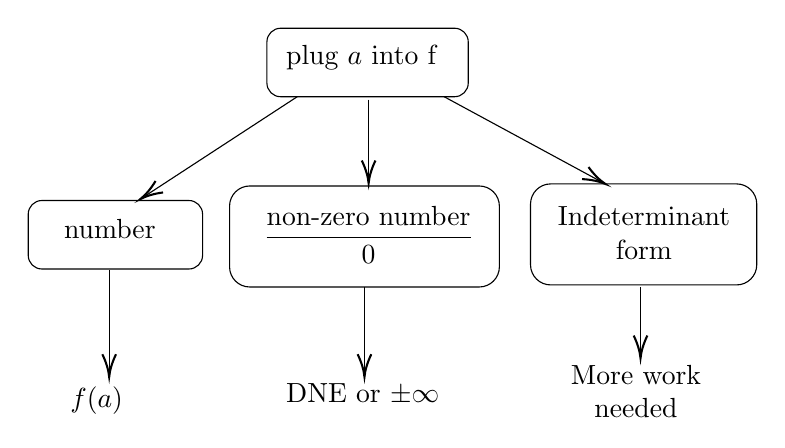
\begin{tikzpicture}[x=0.75pt,y=0.75pt,yscale=-1,xscale=1]
%uncomment if require: \path (0,446); %set diagram left start at 0, and has height of 446

%Rounded Rect [id:dp04536261924917495] 
\draw   (218,91.93) .. controls (218,88.29) and (220.95,85.33) .. (224.6,85.33) -- (308.4,85.33) .. controls (312.05,85.33) and (315,88.29) .. (315,91.93) -- (315,111.73) .. controls (315,115.38) and (312.05,118.33) .. (308.4,118.33) -- (224.6,118.33) .. controls (220.95,118.33) and (218,115.38) .. (218,111.73) -- cycle ;
%Straight Lines [id:da43038695232156465] 
\draw    (232.6,118.33) -- (158.67,166.57) ;
\draw [shift={(157,167.67)}, rotate = 326.87] [color={rgb, 255:red, 0; green, 0; blue, 0 }  ][line width=0.75]    (10.93,-3.29) .. controls (6.95,-1.4) and (3.31,-0.3) .. (0,0) .. controls (3.31,0.3) and (6.95,1.4) .. (10.93,3.29)   ;
%Straight Lines [id:da02535983624938165] 
\draw    (267,119.67) -- (267,158) ;
\draw [shift={(267,160)}, rotate = 270] [color={rgb, 255:red, 0; green, 0; blue, 0 }  ][line width=0.75]    (10.93,-3.29) .. controls (6.95,-1.4) and (3.31,-0.3) .. (0,0) .. controls (3.31,0.3) and (6.95,1.4) .. (10.93,3.29)   ;
%Straight Lines [id:da33645697944263864] 
\draw    (303.4,118.33) -- (379.24,159.38) ;
\draw [shift={(381,160.33)}, rotate = 208.42] [color={rgb, 255:red, 0; green, 0; blue, 0 }  ][line width=0.75]    (10.93,-3.29) .. controls (6.95,-1.4) and (3.31,-0.3) .. (0,0) .. controls (3.31,0.3) and (6.95,1.4) .. (10.93,3.29)   ;
%Rounded Rect [id:dp8149957234073693] 
\draw   (103,174.93) .. controls (103,171.29) and (105.95,168.33) .. (109.6,168.33) -- (180.4,168.33) .. controls (184.05,168.33) and (187,171.29) .. (187,174.93) -- (187,194.73) .. controls (187,198.38) and (184.05,201.33) .. (180.4,201.33) -- (109.6,201.33) .. controls (105.95,201.33) and (103,198.38) .. (103,194.73) -- cycle ;
%Rounded Rect [id:dp9518200785534192] 
\draw   (200,171.07) .. controls (200,165.69) and (204.36,161.33) .. (209.73,161.33) -- (320.27,161.33) .. controls (325.64,161.33) and (330,165.69) .. (330,171.07) -- (330,200.27) .. controls (330,205.64) and (325.64,210) .. (320.27,210) -- (209.73,210) .. controls (204.36,210) and (200,205.64) .. (200,200.27) -- cycle ;
%Rounded Rect [id:dp5380321492603661] 
\draw   (345,170.07) .. controls (345,164.69) and (349.36,160.33) .. (354.73,160.33) -- (444.27,160.33) .. controls (449.64,160.33) and (454,164.69) .. (454,170.07) -- (454,199.27) .. controls (454,204.64) and (449.64,209) .. (444.27,209) -- (354.73,209) .. controls (349.36,209) and (345,204.64) .. (345,199.27) -- cycle ;
%Straight Lines [id:da980017392599877] 
\draw    (142,202) -- (142,251.33) ;
\draw [shift={(142,253.33)}, rotate = 270] [color={rgb, 255:red, 0; green, 0; blue, 0 }  ][line width=0.75]    (10.93,-3.29) .. controls (6.95,-1.4) and (3.31,-0.3) .. (0,0) .. controls (3.31,0.3) and (6.95,1.4) .. (10.93,3.29)   ;
%Straight Lines [id:da24546083605149582] 
\draw    (265,210) -- (265,251.33) ;
\draw [shift={(265,253.33)}, rotate = 270] [color={rgb, 255:red, 0; green, 0; blue, 0 }  ][line width=0.75]    (10.93,-3.29) .. controls (6.95,-1.4) and (3.31,-0.3) .. (0,0) .. controls (3.31,0.3) and (6.95,1.4) .. (10.93,3.29)   ;
%Straight Lines [id:da8582799815353812] 
\draw    (398,210) -- (398,242.33) ;
\draw [shift={(398,244.33)}, rotate = 270] [color={rgb, 255:red, 0; green, 0; blue, 0 }  ][line width=0.75]    (10.93,-3.29) .. controls (6.95,-1.4) and (3.31,-0.3) .. (0,0) .. controls (3.31,0.3) and (6.95,1.4) .. (10.93,3.29)   ;

% Text Node
\draw (226,92.33) node [anchor=north west][inner sep=0.75pt]   [align=left] {plug $\displaystyle a$ into f};
% Text Node
\draw (119,176.33) node [anchor=north west][inner sep=0.75pt]   [align=left] {number};
% Text Node
\draw (355,170) node [anchor=north west][inner sep=0.75pt]   [align=left] {\begin{minipage}[lt]{65.09pt}\setlength\topsep{0pt}
\begin{center}
Indeterminant\\form
\end{center}

\end{minipage}};
% Text Node
\draw (122,256.83) node [anchor=north west][inner sep=0.75pt]   [align=left] {$f(a)$};
% Text Node
\draw (226,255.33) node [anchor=north west][inner sep=0.75pt]   [align=left] {DNE or $\displaystyle \pm \infty $};
% Text Node
\draw (361,246.33) node [anchor=north west][inner sep=0.75pt]   [align=left] {\begin{minipage}[lt]{50.33pt}\setlength\topsep{0pt}
\begin{center}
More work\\needed
\end{center}

\end{minipage}};
% Text Node
\draw (215,170) node [anchor=north west][inner sep=0.75pt]    {$\displaystyle\frac{\text{non-zero number}}{0}$};

\end{tikzpicture}
    }
    \caption{Flowchart for evaluating limits}
    \label{fig:flowchart}
\end{figure}

\subsection{A Number}

If $f$ is an ACCF and $f(a)$ is a number, then $a$ is in the domain of $f$. Since any ACCF is continuous on its domain,
$$\lim_{x\to a}f(x)=f(a)$$
by the definition of continuity. \mar{Re-read this until you understand it!}

\subsection{A (non-zero) Number over Zero}

If $f$ is an ACCF and attempting to evaluate $f(a)$ results in a non-zero number over 0, then $f$ has a vertical asymptote at $x=a$. Near $x=a$, the values of $f(x)$ get very close to either positive or negative infinity. The right and left sided limits are either positive or negative infinity, so there are only four cases, as seen in figure \ref{fig:four-cases}.

\begin{figure}[h]
    \centering
    \fbox{
        \resizebox{4.25in}{!}{
        \tikzset{every picture/.style={line width=0.75pt}} %set default line width to 0.75pt        
        
        \begin{tikzpicture}[x=0.75pt,y=0.75pt,yscale=-1,xscale=1]
        %uncomment if require: \path (0,446); %set diagram left start at 0, and has height of 446
        
        %Straight Lines [id:da7130638550602129] 
        \draw    (17.32,128.98) -- (162.73,128.98) ;
        %Curve Lines [id:da8198586763402247] 
        \draw    (19.1,124.51) .. controls (81.55,124.51) and (86.01,102.21) .. (86.01,57.6) ;
        %Curve Lines [id:da33054163491632704] 
        \draw    (161.84,124.51) .. controls (99.39,124.51) and (94.93,102.21) .. (94.93,57.6) ;
        %Straight Lines [id:da39635263385432795] 
        \draw  [dash pattern={on 0.84pt off 2.51pt}]  (90.47,54.93) -- (90.47,201.24) ;
        
        %Straight Lines [id:da4984898910131832] 
        \draw    (187.51,128.98) -- (332.93,128.98) ;
        %Curve Lines [id:da12653349982399664] 
        \draw    (189.3,124.51) .. controls (251.75,124.51) and (256.21,102.21) .. (256.21,57.6) ;
        %Curve Lines [id:da6963380775085903] 
        \draw    (332.04,133.14) .. controls (269.59,133.14) and (265.13,155.74) .. (265.13,200.05) ;
        %Straight Lines [id:da5434138892345324] 
        \draw  [dash pattern={on 0.84pt off 2.51pt}]  (260.67,54.93) -- (260.67,201.24) ;
        
        %Straight Lines [id:da6992946751383504] 
        \draw    (357.71,128.98) -- (503.13,128.98) ;
        %Curve Lines [id:da5321156852218221] 
        \draw    (359.5,132.54) .. controls (421.95,132.54) and (426.41,155.74) .. (426.41,200.05) ;
        %Curve Lines [id:da8818577355654187] 
        \draw    (502.24,124.51) .. controls (439.79,124.51) and (435.33,102.21) .. (435.33,57.6) ;
        %Straight Lines [id:da23325172919339887] 
        \draw  [dash pattern={on 0.84pt off 2.51pt}]  (430.87,54.93) -- (430.87,201.24) ;
        
        %Straight Lines [id:da2808110791577314] 
        \draw    (527.91,128.98) -- (673.33,128.98) ;
        %Curve Lines [id:da43641618110544544] 
        \draw    (530,133.73) .. controls (592.45,133.73) and (596.91,155.14) .. (596.91,200.05) ;
        %Curve Lines [id:da16583705050218067] 
        \draw    (672.44,133.14) .. controls (609.99,133.14) and (605.53,155.74) .. (605.53,200.05) ;
        %Straight Lines [id:da9264659475889601] 
        \draw  [dash pattern={on 0.84pt off 2.51pt}]  (601.07,54.93) -- (601.07,201.24) ;
        
        
        
        
        
        \end{tikzpicture}
        
        % \resizebox{3in}{!}{
        % \tikzset{every picture/.style={line width=0.75pt}} %set default line width to 0.75pt        
        % \begin{tikzpicture}[x=0.75pt,y=0.75pt,yscale=-1,xscale=1]
        % %uncomment if require: \path (0,446); %set diagram left start at 0, and has height of 446
        
        % %Straight Lines [id:da11666177611802953] 
        % \draw    (98,120.33) -- (261,120.33) ;
        % %Curve Lines [id:da20823749405635383] 
        % \draw    (100,115.33) .. controls (170,115.33) and (175,90.33) .. (175,40.33) ;
        % %Curve Lines [id:da5857981133236727] 
        % \draw    (260,115.33) .. controls (190,115.33) and (185,90.33) .. (185,40.33) ;
        % %Straight Lines [id:da8270643292998765] 
        % \draw  [dash pattern={on 0.84pt off 2.51pt}]  (180,37.33) -- (180,201.33) ;
        
        % %Straight Lines [id:da6737028355731796] 
        % \draw    (288,120.33) -- (451,120.33) ;
        % %Curve Lines [id:da5853120673537593] 
        % \draw    (290,115.33) .. controls (360,115.33) and (365,90.33) .. (365,40.33) ;
        % %Curve Lines [id:da33546715055487053] 
        % \draw    (450,125) .. controls (380,125) and (375,150.33) .. (375,200) ;
        % %Straight Lines [id:da39333458455778736] 
        % \draw  [dash pattern={on 0.84pt off 2.51pt}]  (370,37.33) -- (370,201.33) ;
        
        
        % %Straight Lines [id:da41843468171367526] 
        % \draw    (98,310.33) -- (261,310.33) ;
        % %Curve Lines [id:da9482877395734075] 
        % \draw    (100,314.33) .. controls (170,314.33) and (175,340.33) .. (175,390) ;
        % %Curve Lines [id:da7803855380541431] 
        % \draw    (260,305.33) .. controls (190,305.33) and (185,280.33) .. (185,230.33) ;
        % %Straight Lines [id:da11027576459803168] 
        % \draw  [dash pattern={on 0.84pt off 2.51pt}]  (180,227.33) -- (180,391.33) ;
        
        % %Straight Lines [id:da294114983098098] 
        % \draw    (288,310.33) -- (451,310.33) ;
        % %Curve Lines [id:da491751074451225] 
        % \draw    (290.33,315.67) .. controls (360.33,315.67) and (365.33,339.67) .. (365.33,390) ;
        % %Curve Lines [id:da32646541541064433] 
        % \draw    (450,315) .. controls (380,315) and (375,340.33) .. (375,390) ;
        % %Straight Lines [id:da20001269749677508] 
        % \draw  [dash pattern={on 0.84pt off 2.51pt}]  (370,227.33) -- (370,391.33) ;
        
        
        
        
        
        
        % \end{tikzpicture}
        % }
        }
    }
    \caption{The four cases of vertical asymptotes}
    \label{fig:four-cases}
\end{figure}

Therefore, the only possibilities for the value of these limits are $\infty$, $-\infty$, and DNE. \mar{Label each function in figure \ref{fig:four-cases} with its respective limit.} To figure it out which one it is, evaluate both of the two sided limits. For each, plug in a value that is slightly to the right (or the left) of $a$. If the result is positive, the sided limit is positive infinity, and if the result is negative, negative infinity.

\subsection{Indeterminant Form}

There are seven indeterminant forms:

\vspace{1em}

\begin{center}
\begin{Large}
\phantom{}\hfill
$\frac{0}{0}$ \hfill
$\frac{\infty}{\infty}$ \hfill
$0^0$ \hfill
$\infty{-}\infty$ \hfill
$1^\infty$ \hfill
$0{\cdot}\infty$ \hfill
$\infty^0$
\hfill\phantom{}
\end{Large}
\end{center}

\vspace{1em}

They are called \textbf{indeterminant} because in this form, we cannot be sure of its value (or even if its value makes sense). Take $0^0$ for example: zero raised to any power should be 0, but anything raised to the power of $0$ should be 1... so which is it? \mar{Write out similar question for the other 6 indeterminant forms.}

When we get an indeterminant form after trying to evaluate $f(a)$, we need to do more work. There are several things you can try:

\begin{itemize}
\item Simplify. If the function is rational and has common factor in its numerator and denominator, by ``canceling'' the term, the resulting function is not the same: the original function has a hole at the point where the factored term is 0. For example, $f(x)=\frac{x(x-1)}{(x-1)}$ has a hole at $x=1$, but everywhere else is the line $y=x$. However, this cancellation does not change the value of the limit.
\item Multiply the numerator and denominator of a rational function by the conjugate of the denominator or the numerator (the \textbf{conjugate} of a binomial $a+b$ is $a-b$).
\item Use a special-case limit: 
$$
\lim_{x\to 0}\frac{\sin(x)}{x} = 1
\quad\quad\quad\quad
\lim_{x\to 0}\frac{\cos(x) - 1}{x} = 0
$$
$$
\lim_{x\to\infty}\left(1+\frac{1}{x}\right)^x = e
\quad\quad\quad\quad
\lim_{x\to 0}\frac{a^x-1}{x}=\ln(a)
$$

\item In the case of $x\to\pm\infty$ for a rational function, divide the numerator and denominator by the highest degree term of the denominator.

\item Use the Squeeze Theorem:

\begin{thm}[Squeeze Theorem]
Let $f$, $g$, and $h$ be functions with $g(x)\leq f(x)\leq h(x)$ for all $x$ in some interval around $a$ (except possibly at $a$). If $$\lim_{x\to a}g(x)=L=\lim_{x\to a} h(x),$$ then $$\lim_{x\to a} f(x)=L$$
as well.
\end{thm}
The most common application of squeeze theorem is squeezing $$-1\leq \sin\theta \leq 1.$$

\end{itemize}

Later, we will learn a trick called L'H\^opital's Rule to more easily compute limits with indeterminant forms. But first we need to learn about derivatives!













% \section{Limits}

Limits are important in calculus since we need very small quantities to effectively study change. Yeah, that's pretty vague, but hopefully it'll clear up in a few pages.

We study limits for many reasons. One of them is to study functions at points where they are only ``close'' to being defined. For example, the function $f$ given by $f(x)=\frac{x(x+1)}{x}$ is not defined at $0$, but looks like the line $x+1$ everywhere else.

\subsection{Intuitive Limits}

The intuitive idea of a \textbf{limit} is to examine what the output of a function does as the input moves close to a specific value. Since the functions we care about take real numbers as inputs, there are two ways you can approach a number on the real line (from the left and from the right). We will talk about left- and right-sided limits.

Before getting into the actual definition, we'll start intuitively. If a function is     ``continuous''\footnote{I put this word in quotes because I haven't defined it yet, but you should have an intuitive idea of what this means: being able to draw it without lifting your pencil. Just wait for a few pages.} and is defined at $a$, then as $x$ moves closer to $a$, $f(x)$ moves closer to $f(a)$, so the limit of $f$ as $x$ approaches $a$ is $f(a)$.


Let's get a little more general: suppose a function $f$ is defined on open intervals on either side of $a$.

If $f$ is defined on an interval to the \textit{left} of $a$ and the values of $f(x)$ approach $L$ as $x$ approaches $a$ from the \textit{left}, we say that the ``\textbf{left-sided limit of $f$ as $x$ approaches $a$} is $L$'' and we write $$\lim_{x\to a^-}f(x)=L.$$
If $f$ is defined on an interval to the \textit{right} of $a$ and the values of $f(x)$ approach $L$ as $x$ approaches $a$ from the \textit{right}, we say that the \textbf{right-sided limit of $f$ as $x$ approaches $a$} is $L$'' and we write
$$\lim_{x\to a^+}f(x)=L.$$
If the right and left sided limits match, then we say that the \textbf{limit of $f$ as $x$ approaches $a$ is $L$} and write $$\lim_{x\to a}f(x)=L.$$

\noindent Note: $f$ need not be defined at $a$ to find the limit of $f$ as $x$ approaches $a$.

\vspace{1em}

One can compute $f(x)$ for values of $x$ that get closer and closer to either side of $a$. If the values approach $L$, then you have good reason to believe that $L$ is the (right- and/or left-sided) limit.

\begin{center}
\begin{tabular}{@{}ll@{}}
\toprule[0.4mm]
   $x$        & $f(x)$        \\
\midrule
   $a-0.1$    & $f(a-0.1)$    \\
   $a-0.01$   & $f(a-0.01)$   \\
   $a-0.001$  & $f(a-0.001)$  \\
   $a-0.0001$ & $f(a-0.0001)$ \\
\midrule
   $a+0.0001$ & $f(a+0.0001)$ \\
   $a+0.001$  & $f(a+0.001)$  \\
   $a+0.01$   & $f(a+0.01)$   \\
   $a+0.1$    & $f(a+0.1)$    \\
\bottomrule[0.4mm]
\end{tabular}
\end{center}

Such calculations, however, cannot prove that a function limits to a specific value.

\subsection{Infinite Limits}

We can extend the idea of limits outside of the real numbers to include positive and negative infinity in place of both $a$ and $L$.
\begin{itemize}
\item If $f(x)$ grows without bound as $x$ approaches $a$ from the left, then we write $$\lim_{x\to a^-}f(x)=\infty.$$
(Similarly for $x$ approaching $a$ from the right, and also if $f(x)$ becomes increasingly negative without bound).
\item We denote the value (if such a value exists) that $f(x)$ approaches as $x$ approaches $\infty$ as $$\lim_{x\to\infty} f(x).$$
(Similarly if $x$ approaches $-\infty$).
\end{itemize}



\subsection{Optional: The $\varepsilon-\delta$ Definition}

You may be dissatisfied with the intuitive approach to limits, so we can make the definition more rigorous. The main idea that needs to be captured by a formal definition is \textit{arbitrary precision}. That is, we need a way to say formally that ``$f(x)$ approaches $L$ as $x$ approaches $a$.''

By controlling the input $x$, we must be able to make the distance $|f(x)-L|$ between the output $f(x)$ and $L$ to be as small as we want (``arbitrarily small''). In other words, if $\varepsilon>0$ is any small positive number, we must be able to ensure (by controlling $x$) that $|f(x)-L| < \varepsilon$. To control $x$, we can make the distance $|x-a|$ between $x$ and $a$ smaller than some positive number $\delta > 0$ (that may depend on $\varepsilon$).

Now we're ready for the real ``$\varepsilon-\delta$'' definition of a limit: we say that \textbf{$L$ is the limit of $f$ as $x$ approaches $a$} if
$$\text{for all } \varepsilon > 0, \text{ there is some } \delta > 0, \text{ such that } |x - a| < \delta \implies |f(x) - L| <\varepsilon.$$

Read that last line a few times, because statements with multiple quantifiers can be tricky!

\begin{figure}[h!]
\centering
\fbox{
\tikzset{every picture/.style={line width=0.75pt}}
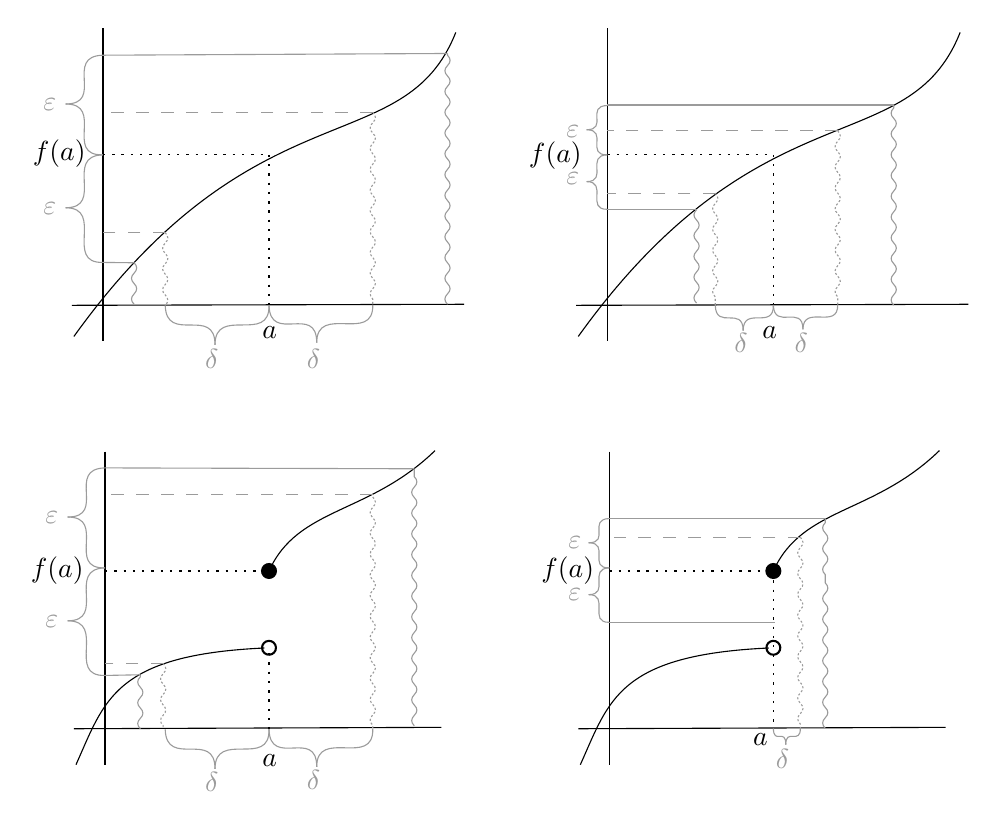
\begin{tikzpicture}[x=0.75pt,y=0.75pt,yscale=-1,xscale=1]
%uncomment if require: \path (0,428); %set diagram left start at 0, and has height of 428

%Straight Lines [id:da2730924968926851]
\draw    (71,155) -- (260,154.5) ;
%Straight Lines [id:da38663844155403493]
\draw    (86,21.5) -- (86,172.33) ;
%Curve Lines [id:da5832897062677318]
\draw    (72,170) .. controls (160,47.5) and (231,86.5) .. (256,23.5) ;
%Curve Lines [id:da15926967534570857]
\draw    (73,376.33) .. controls (86.86,345.64) and (90.92,323.45) .. (163.77,320.1) ;
\draw [shift={(166,320)}, rotate = 357.71] [color={rgb, 255:red, 0; green, 0; blue, 0 }  ][line width=0.75]      (0, 0) circle [x radius= 3.35, y radius= 3.35]   ;
%Curve Lines [id:da573129079856388]
\draw    (166,283) .. controls (180,252) and (214,256) .. (246,225) ;
\draw [shift={(166,283)}, rotate = 294.3] [color={rgb, 255:red, 0; green, 0; blue, 0 }  ][fill={rgb, 255:red, 0; green, 0; blue, 0 }  ][line width=0.75]      (0, 0) circle [x radius= 3.35, y radius= 3.35]   ;
%Straight Lines [id:da06544192635535961]
\draw  [dash pattern={on 0.84pt off 2.51pt}]  (166,82.5) -- (166,154.92) ;
%Straight Lines [id:da8462520068785757]
\draw  [dash pattern={on 0.84pt off 2.51pt}]  (86,82.5) -- (166,82.5) ;
%Straight Lines [id:da8033956316212987]
\draw [color={rgb, 255:red, 155; green, 155; blue, 155 }  ,draw opacity=1 ]   (86,34.5) -- (252,33.67) ;
%Straight Lines [id:da9058328806059841]
\draw [color={rgb, 255:red, 155; green, 155; blue, 155 }  ,draw opacity=1 ]   (86,134.33) -- (101,134.5) ;
%Straight Lines [id:da7683874289412185]
\draw    (72,359) -- (249,358.33) ;
%Straight Lines [id:da21021021460529377]
\draw    (87,225.5) -- (87,376.33) ;
%Straight Lines [id:da5263630709862186]
\draw  [dash pattern={on 0.84pt off 2.51pt}]  (166,322.58) -- (166,359.25) ;
%Straight Lines [id:da2255352189878881]
\draw  [dash pattern={on 0.84pt off 2.51pt}]  (87,283) -- (166,283) ;
%Straight Lines [id:da12241776303117424]
\draw [color={rgb, 255:red, 155; green, 155; blue, 155 }  ,draw opacity=1 ]   (87,233.33) -- (236,233.75) ;
%Straight Lines [id:da6551551228954233]
\draw [color={rgb, 255:red, 155; green, 155; blue, 155 }  ,draw opacity=1 ]   (87,333.33) -- (104,333) ;
%Straight Lines [id:da3470258564776276]
\draw [color={rgb, 255:red, 155; green, 155; blue, 155 }  ,draw opacity=1 ] [dash pattern={on 0.75pt off 0.75pt}]  (116,120) .. controls (117.67,121.67) and (117.67,123.33) .. (116,125) .. controls (114.33,126.67) and (114.33,128.33) .. (116,130) .. controls (117.67,131.67) and (117.67,133.33) .. (116,135) .. controls (114.33,136.67) and (114.33,138.33) .. (116,140) .. controls (117.67,141.67) and (117.67,143.33) .. (116,145) .. controls (114.33,146.67) and (114.33,148.33) .. (116,150) .. controls (117.67,151.67) and (117.67,153.33) .. (116,155) -- (116,155) ;
%Straight Lines [id:da2371091562631653]
\draw [color={rgb, 255:red, 155; green, 155; blue, 155 }  ,draw opacity=1 ] [dash pattern={on 0.75pt off 0.75pt}]  (216,62) .. controls (217.67,63.67) and (217.67,65.33) .. (216,67) .. controls (214.33,68.67) and (214.33,70.33) .. (216,72) .. controls (217.67,73.67) and (217.67,75.33) .. (216,77) .. controls (214.33,78.67) and (214.33,80.33) .. (216,82) .. controls (217.67,83.67) and (217.67,85.33) .. (216,87) .. controls (214.33,88.67) and (214.33,90.33) .. (216,92) .. controls (217.67,93.67) and (217.67,95.33) .. (216,97) .. controls (214.33,98.67) and (214.33,100.33) .. (216,102) .. controls (217.67,103.67) and (217.67,105.33) .. (216,107) .. controls (214.33,108.67) and (214.33,110.33) .. (216,112) .. controls (217.67,113.67) and (217.67,115.33) .. (216,117) .. controls (214.33,118.67) and (214.33,120.33) .. (216,122) .. controls (217.67,123.67) and (217.67,125.33) .. (216,127) .. controls (214.33,128.67) and (214.33,130.33) .. (216,132) .. controls (217.67,133.67) and (217.67,135.33) .. (216,137) .. controls (214.33,138.67) and (214.33,140.33) .. (216,142) .. controls (217.67,143.67) and (217.67,145.33) .. (216,147) .. controls (214.33,148.67) and (214.33,150.33) .. (216,152) -- (216,154.71) -- (216,154.71) ;
%Straight Lines [id:da47940446384008517]
\draw [color={rgb, 255:red, 155; green, 155; blue, 155 }  ,draw opacity=1 ] [dash pattern={on 4.5pt off 4.5pt}]  (116,120) -- (86,120) ;
%Straight Lines [id:da2718218581855085]
\draw [color={rgb, 255:red, 155; green, 155; blue, 155 }  ,draw opacity=1 ] [dash pattern={on 4.5pt off 4.5pt}]  (216,62) -- (86,62) ;
%Curve Lines [id:da7867325499156288]
\draw [color={rgb, 255:red, 155; green, 155; blue, 155 }  ,draw opacity=1 ]   (68,58) .. controls (87,58) and (67,35) .. (86,34.5) ;
%Curve Lines [id:da8389021578247982]
\draw [color={rgb, 255:red, 155; green, 155; blue, 155 }  ,draw opacity=1 ]   (68,58) .. controls (87,58) and (67,83) .. (86,82.5) ;
%Curve Lines [id:da6940267896547274]
\draw [color={rgb, 255:red, 155; green, 155; blue, 155 }  ,draw opacity=1 ]   (68,108) .. controls (87,108) and (67,83) .. (86,82.5) ;
%Curve Lines [id:da9368251006708403]
\draw [color={rgb, 255:red, 155; green, 155; blue, 155 }  ,draw opacity=1 ]   (68,108) .. controls (87,108) and (67,134.83) .. (86,134.33) ;
%Curve Lines [id:da7416463958304471]
\draw [color={rgb, 255:red, 155; green, 155; blue, 155 }  ,draw opacity=1 ]   (139.99,174) .. controls (140,155) and (116.5,174) .. (116,155) ;
%Curve Lines [id:da0946019041451891]
\draw [color={rgb, 255:red, 155; green, 155; blue, 155 }  ,draw opacity=1 ]   (139.99,174) .. controls (140,155) and (166.5,173.92) .. (166,154.92) ;
%Curve Lines [id:da8479225025412045]
\draw [color={rgb, 255:red, 155; green, 155; blue, 155 }  ,draw opacity=1 ]   (188.99,173) .. controls (189,154) and (166.5,173.92) .. (166,154.92) ;
%Curve Lines [id:da5287374586288269]
\draw [color={rgb, 255:red, 155; green, 155; blue, 155 }  ,draw opacity=1 ]   (188.99,173) .. controls (189,154) and (216.5,173.71) .. (216,154.71) ;
%Straight Lines [id:da5763369512697336]
\draw [color={rgb, 255:red, 155; green, 155; blue, 155 }  ,draw opacity=1 ]   (101,154.5) .. controls (99.33,152.83) and (99.33,151.17) .. (101,149.5) .. controls (102.67,147.83) and (102.67,146.17) .. (101,144.5) .. controls (99.33,142.83) and (99.33,141.17) .. (101,139.5) .. controls (102.67,137.83) and (102.67,136.17) .. (101,134.5) -- (101,134.5) ;
%Straight Lines [id:da9925497456851824]
\draw [color={rgb, 255:red, 155; green, 155; blue, 155 }  ,draw opacity=1 ]   (252,154.5) .. controls (250.33,152.83) and (250.33,151.17) .. (252,149.5) .. controls (253.67,147.83) and (253.67,146.17) .. (252,144.5) .. controls (250.33,142.83) and (250.33,141.17) .. (252,139.5) .. controls (253.67,137.83) and (253.67,136.17) .. (252,134.5) .. controls (250.33,132.83) and (250.33,131.17) .. (252,129.5) .. controls (253.67,127.83) and (253.67,126.17) .. (252,124.5) .. controls (250.33,122.83) and (250.33,121.17) .. (252,119.5) .. controls (253.67,117.83) and (253.67,116.17) .. (252,114.5) .. controls (250.33,112.83) and (250.33,111.17) .. (252,109.5) .. controls (253.67,107.83) and (253.67,106.17) .. (252,104.5) .. controls (250.33,102.83) and (250.33,101.17) .. (252,99.5) .. controls (253.67,97.83) and (253.67,96.17) .. (252,94.5) .. controls (250.33,92.83) and (250.33,91.17) .. (252,89.5) .. controls (253.67,87.83) and (253.67,86.17) .. (252,84.5) .. controls (250.33,82.83) and (250.33,81.17) .. (252,79.5) .. controls (253.67,77.83) and (253.67,76.17) .. (252,74.5) .. controls (250.33,72.83) and (250.33,71.17) .. (252,69.5) .. controls (253.67,67.83) and (253.67,66.17) .. (252,64.5) .. controls (250.33,62.83) and (250.33,61.17) .. (252,59.5) .. controls (253.67,57.83) and (253.67,56.17) .. (252,54.5) .. controls (250.33,52.83) and (250.33,51.17) .. (252,49.5) .. controls (253.67,47.83) and (253.67,46.17) .. (252,44.5) .. controls (250.33,42.83) and (250.33,41.17) .. (252,39.5) .. controls (253.67,37.83) and (253.67,36.17) .. (252,34.5) -- (252,33.67) -- (252,33.67) ;
%Curve Lines [id:da7131476230234577]
\draw [color={rgb, 255:red, 155; green, 155; blue, 155 }  ,draw opacity=1 ]   (69,257) .. controls (88,257) and (68,233.83) .. (87,233.33) ;
%Curve Lines [id:da5212410455410692]
\draw [color={rgb, 255:red, 155; green, 155; blue, 155 }  ,draw opacity=1 ]   (69,257) .. controls (88,257) and (68,282) .. (87,281.5) ;
%Curve Lines [id:da8037674418363849]
\draw [color={rgb, 255:red, 155; green, 155; blue, 155 }  ,draw opacity=1 ]   (69,307) .. controls (88,307) and (68,282) .. (87,281.5) ;
%Curve Lines [id:da3061502012065347]
\draw [color={rgb, 255:red, 155; green, 155; blue, 155 }  ,draw opacity=1 ]   (69,307) .. controls (88,307) and (68,333.83) .. (87,333.33) ;
%Curve Lines [id:da838846723146208]
\draw [color={rgb, 255:red, 155; green, 155; blue, 155 }  ,draw opacity=1 ]   (139.99,378.34) .. controls (140,359.34) and (116.5,378.33) .. (116,359.33) ;
%Curve Lines [id:da45926415056497105]
\draw [color={rgb, 255:red, 155; green, 155; blue, 155 }  ,draw opacity=1 ]   (139.99,378.34) .. controls (140,359.34) and (166.5,378.25) .. (166,359.25) ;
%Curve Lines [id:da1812164249288335]
\draw [color={rgb, 255:red, 155; green, 155; blue, 155 }  ,draw opacity=1 ]   (188.99,377.34) .. controls (189,358.34) and (166.5,378.25) .. (166,359.25) ;
%Curve Lines [id:da5310165714599331]
\draw [color={rgb, 255:red, 155; green, 155; blue, 155 }  ,draw opacity=1 ]   (188.99,377.34) .. controls (189,358.34) and (216.5,378.04) .. (216,359.04) ;
%Straight Lines [id:da1373743464903565]
\draw [color={rgb, 255:red, 155; green, 155; blue, 155 }  ,draw opacity=1 ] [dash pattern={on 0.75pt off 0.75pt}]  (115,327.5) .. controls (116.67,329.17) and (116.67,330.83) .. (115,332.5) .. controls (113.33,334.17) and (113.33,335.83) .. (115,337.5) .. controls (116.67,339.17) and (116.67,340.83) .. (115,342.5) .. controls (113.33,344.17) and (113.33,345.83) .. (115,347.5) .. controls (116.67,349.17) and (116.67,350.83) .. (115,352.5) .. controls (113.33,354.17) and (113.33,355.83) .. (115,357.5) -- (115,359) -- (115,359) ;
%Straight Lines [id:da30273639101181327]
\draw [color={rgb, 255:red, 155; green, 155; blue, 155 }  ,draw opacity=1 ] [dash pattern={on 0.75pt off 0.75pt}]  (216,247.33) .. controls (217.67,249) and (217.67,250.66) .. (216,252.33) .. controls (214.33,254) and (214.33,255.66) .. (216,257.33) .. controls (217.67,259) and (217.67,260.66) .. (216,262.33) .. controls (214.33,264) and (214.33,265.66) .. (216,267.33) .. controls (217.67,269) and (217.67,270.66) .. (216,272.33) .. controls (214.33,274) and (214.33,275.66) .. (216,277.33) .. controls (217.67,279) and (217.67,280.66) .. (216,282.33) .. controls (214.33,284) and (214.33,285.66) .. (216,287.33) .. controls (217.67,289) and (217.67,290.66) .. (216,292.33) .. controls (214.33,294) and (214.33,295.66) .. (216,297.33) .. controls (217.67,299) and (217.67,300.66) .. (216,302.33) .. controls (214.33,304) and (214.33,305.66) .. (216,307.33) .. controls (217.67,309) and (217.67,310.66) .. (216,312.33) .. controls (214.33,314) and (214.33,315.66) .. (216,317.33) .. controls (217.67,319) and (217.67,320.66) .. (216,322.33) .. controls (214.33,324) and (214.33,325.66) .. (216,327.33) .. controls (217.67,329) and (217.67,330.66) .. (216,332.33) .. controls (214.33,334) and (214.33,335.66) .. (216,337.33) .. controls (217.67,339) and (217.67,340.66) .. (216,342.33) .. controls (214.33,344) and (214.33,345.66) .. (216,347.33) .. controls (217.67,349) and (217.67,350.66) .. (216,352.33) .. controls (214.33,354) and (214.33,355.66) .. (216,357.33) -- (216,359.04) -- (216,359.04) ;
%Straight Lines [id:da6690760580285089]
\draw [color={rgb, 255:red, 155; green, 155; blue, 155 }  ,draw opacity=1 ] [dash pattern={on 4.5pt off 4.5pt}]  (115,327.5) -- (87,327.5) ;
%Straight Lines [id:da023392902319420816]
\draw [color={rgb, 255:red, 155; green, 155; blue, 155 }  ,draw opacity=1 ] [dash pattern={on 4.5pt off 4.5pt}]  (216,246) -- (87,246) ;
%Straight Lines [id:da7002803226646901]
\draw [color={rgb, 255:red, 155; green, 155; blue, 155 }  ,draw opacity=1 ]   (104,359) .. controls (102.33,357.33) and (102.33,355.67) .. (104,354) .. controls (105.67,352.33) and (105.67,350.67) .. (104,349) .. controls (102.33,347.33) and (102.33,345.67) .. (104,344) .. controls (105.67,342.33) and (105.67,340.67) .. (104,339) .. controls (102.33,337.33) and (102.33,335.67) .. (104,334) -- (104,333) -- (104,333) ;
%Straight Lines [id:da5440309336359443]
\draw [color={rgb, 255:red, 155; green, 155; blue, 155 }  ,draw opacity=1 ]   (236,357.58) .. controls (234.33,355.91) and (234.33,354.25) .. (236,352.58) .. controls (237.67,350.91) and (237.67,349.25) .. (236,347.58) .. controls (234.33,345.91) and (234.33,344.25) .. (236,342.58) .. controls (237.67,340.91) and (237.67,339.25) .. (236,337.58) .. controls (234.33,335.91) and (234.33,334.25) .. (236,332.58) .. controls (237.67,330.91) and (237.67,329.25) .. (236,327.58) .. controls (234.33,325.91) and (234.33,324.25) .. (236,322.58) .. controls (237.67,320.91) and (237.67,319.25) .. (236,317.58) .. controls (234.33,315.91) and (234.33,314.25) .. (236,312.58) .. controls (237.67,310.91) and (237.67,309.25) .. (236,307.58) .. controls (234.33,305.91) and (234.33,304.25) .. (236,302.58) .. controls (237.67,300.91) and (237.67,299.25) .. (236,297.58) .. controls (234.33,295.91) and (234.33,294.25) .. (236,292.58) .. controls (237.67,290.91) and (237.67,289.25) .. (236,287.58) .. controls (234.33,285.91) and (234.33,284.25) .. (236,282.58) .. controls (237.67,280.91) and (237.67,279.25) .. (236,277.58) .. controls (234.33,275.91) and (234.33,274.25) .. (236,272.58) .. controls (237.67,270.91) and (237.67,269.25) .. (236,267.58) .. controls (234.33,265.91) and (234.33,264.25) .. (236,262.58) .. controls (237.67,260.91) and (237.67,259.25) .. (236,257.58) .. controls (234.33,255.91) and (234.33,254.25) .. (236,252.58) .. controls (237.67,250.91) and (237.67,249.25) .. (236,247.58) .. controls (234.33,245.91) and (234.33,244.25) .. (236,242.58) .. controls (237.67,240.91) and (237.67,239.25) .. (236,237.58) -- (236,233.75) -- (236,233.75) ;

%Straight Lines [id:da8513462018635212]
\draw    (314,155) -- (503,154.5) ;
%Straight Lines [id:da27501056686778513]
\draw    (329,21.5) -- (329,172.33) ;
%Curve Lines [id:da5516996470591613]
\draw    (315,170) .. controls (403,47.5) and (474,86.5) .. (499,23.5) ;
%Curve Lines [id:da2905586367584121]
\draw    (316,376.33) .. controls (329.86,345.64) and (333.92,323.45) .. (406.77,320.1) ;
\draw [shift={(409,320)}, rotate = 357.71] [color={rgb, 255:red, 0; green, 0; blue, 0 }  ][line width=0.75]      (0, 0) circle [x radius= 3.35, y radius= 3.35]   ;
%Curve Lines [id:da17327963328411955]
\draw    (409,283) .. controls (423,252) and (457,256) .. (489,225) ;
\draw [shift={(409,283)}, rotate = 294.3] [color={rgb, 255:red, 0; green, 0; blue, 0 }  ][fill={rgb, 255:red, 0; green, 0; blue, 0 }  ][line width=0.75]      (0, 0) circle [x radius= 3.35, y radius= 3.35]   ;
%Straight Lines [id:da4442118515906792]
\draw  [dash pattern={on 0.84pt off 2.51pt}]  (409,82.5) -- (409,154.92) ;
%Straight Lines [id:da4615400041448172]
\draw  [dash pattern={on 0.84pt off 2.51pt}]  (329,82.5) -- (409,82.5) ;
%Straight Lines [id:da9140897903442382]
\draw [color={rgb, 255:red, 155; green, 155; blue, 155 }  ,draw opacity=1 ]   (329,58.5) -- (467,58.5) ;
%Straight Lines [id:da8879320022705979]
\draw [color={rgb, 255:red, 155; green, 155; blue, 155 }  ,draw opacity=1 ]   (329,108.73) -- (372,108.73) ;
%Straight Lines [id:da17895890987358554]
\draw    (315,359) -- (492,358.33) ;
%Straight Lines [id:da05857321637633417]
\draw    (330,225.5) -- (330,376.33) ;
%Straight Lines [id:da07307770178123163]
\draw  [dash pattern={on 0.84pt off 2.51pt}]  (409,283) -- (409,359.25) ;
%Straight Lines [id:da06234038795466201]
\draw  [dash pattern={on 0.84pt off 2.51pt}]  (330,283) -- (409,283) ;
%Straight Lines [id:da8599377579018705]
\draw [color={rgb, 255:red, 155; green, 155; blue, 155 }  ,draw opacity=1 ]   (330,257.73) -- (434,257.73) ;
%Straight Lines [id:da9417232436931344]
\draw [color={rgb, 255:red, 155; green, 155; blue, 155 }  ,draw opacity=1 ]   (330,307.73) -- (410,307.73) ;
%Straight Lines [id:da21280146915905584]
\draw [color={rgb, 255:red, 155; green, 155; blue, 155 }  ,draw opacity=1 ] [dash pattern={on 0.75pt off 0.75pt}]  (381,100.93) .. controls (382.67,102.6) and (382.67,104.26) .. (381,105.93) .. controls (379.33,107.6) and (379.33,109.26) .. (381,110.93) .. controls (382.67,112.6) and (382.67,114.26) .. (381,115.93) .. controls (379.33,117.6) and (379.33,119.26) .. (381,120.93) .. controls (382.67,122.6) and (382.67,124.26) .. (381,125.93) .. controls (379.33,127.6) and (379.33,129.26) .. (381,130.93) .. controls (382.67,132.6) and (382.67,134.26) .. (381,135.93) .. controls (379.33,137.6) and (379.33,139.26) .. (381,140.93) .. controls (382.67,142.6) and (382.67,144.26) .. (381,145.93) .. controls (379.33,147.6) and (379.33,149.26) .. (381,150.93) -- (381,154.9) -- (381,154.9) ;
%Straight Lines [id:da1757874388402605]
\draw [color={rgb, 255:red, 155; green, 155; blue, 155 }  ,draw opacity=1 ] [dash pattern={on 0.75pt off 0.75pt}]  (440,70.93) .. controls (441.67,72.6) and (441.67,74.26) .. (440,75.93) .. controls (438.33,77.6) and (438.33,79.26) .. (440,80.93) .. controls (441.67,82.6) and (441.67,84.26) .. (440,85.93) .. controls (438.33,87.6) and (438.33,89.26) .. (440,90.93) .. controls (441.67,92.6) and (441.67,94.26) .. (440,95.93) .. controls (438.33,97.6) and (438.33,99.26) .. (440,100.93) .. controls (441.67,102.6) and (441.67,104.26) .. (440,105.93) .. controls (438.33,107.6) and (438.33,109.26) .. (440,110.93) .. controls (441.67,112.6) and (441.67,114.26) .. (440,115.93) .. controls (438.33,117.6) and (438.33,119.26) .. (440,120.93) .. controls (441.67,122.6) and (441.67,124.26) .. (440,125.93) .. controls (438.33,127.6) and (438.33,129.26) .. (440,130.93) .. controls (441.67,132.6) and (441.67,134.26) .. (440,135.93) .. controls (438.33,137.6) and (438.33,139.26) .. (440,140.93) .. controls (441.67,142.6) and (441.67,144.26) .. (440,145.93) .. controls (438.33,147.6) and (438.33,149.26) .. (440,150.93) -- (440,154.71) -- (440,154.71) ;
%Straight Lines [id:da4275079323186526]
\draw [color={rgb, 255:red, 155; green, 155; blue, 155 }  ,draw opacity=1 ] [dash pattern={on 4.5pt off 4.5pt}]  (381,100.93) -- (329,100.93) ;
%Straight Lines [id:da4596336138709165]
\draw [color={rgb, 255:red, 155; green, 155; blue, 155 }  ,draw opacity=1 ] [dash pattern={on 4.5pt off 4.5pt}]  (440,70.93) -- (329,70.93) ;
%Curve Lines [id:da6338318263176852]
\draw [color={rgb, 255:red, 155; green, 155; blue, 155 }  ,draw opacity=1 ]   (394.44,167.24) .. controls (394.44,154.9) and (381.28,167.24) .. (381,154.9) ;
%Curve Lines [id:da34761840807493516]
\draw [color={rgb, 255:red, 155; green, 155; blue, 155 }  ,draw opacity=1 ]   (394.44,167.24) .. controls (394.44,154.9) and (409.28,167.19) .. (409,154.84) ;
%Curve Lines [id:da25995298856914184]
\draw [color={rgb, 255:red, 155; green, 155; blue, 155 }  ,draw opacity=1 ]   (423.25,166.59) .. controls (423.26,154.25) and (409.31,167.19) .. (409,154.84) ;
%Curve Lines [id:da7818991925364918]
\draw [color={rgb, 255:red, 155; green, 155; blue, 155 }  ,draw opacity=1 ]   (423.25,166.59) .. controls (423.26,154.25) and (440.3,167.05) .. (440,154.71) ;
%Straight Lines [id:da007122223942663375]
\draw [color={rgb, 255:red, 155; green, 155; blue, 155 }  ,draw opacity=1 ]   (372,153.93) .. controls (370.33,152.26) and (370.33,150.6) .. (372,148.93) .. controls (373.67,147.26) and (373.67,145.6) .. (372,143.93) .. controls (370.33,142.26) and (370.33,140.6) .. (372,138.93) .. controls (373.67,137.26) and (373.67,135.6) .. (372,133.93) .. controls (370.33,132.26) and (370.33,130.6) .. (372,128.93) .. controls (373.67,127.26) and (373.67,125.6) .. (372,123.93) .. controls (370.33,122.26) and (370.33,120.6) .. (372,118.93) .. controls (373.67,117.26) and (373.67,115.6) .. (372,113.93) .. controls (370.33,112.26) and (370.33,110.6) .. (372,108.93) -- (372,108.73) -- (372,108.73) ;
%Straight Lines [id:da2226129700521089]
\draw [color={rgb, 255:red, 155; green, 155; blue, 155 }  ,draw opacity=1 ]   (467,154.93) .. controls (465.33,153.26) and (465.33,151.6) .. (467,149.93) .. controls (468.67,148.26) and (468.67,146.6) .. (467,144.93) .. controls (465.33,143.26) and (465.33,141.6) .. (467,139.93) .. controls (468.67,138.26) and (468.67,136.6) .. (467,134.93) .. controls (465.33,133.26) and (465.33,131.6) .. (467,129.93) .. controls (468.67,128.26) and (468.67,126.6) .. (467,124.93) .. controls (465.33,123.26) and (465.33,121.6) .. (467,119.93) .. controls (468.67,118.26) and (468.67,116.6) .. (467,114.93) .. controls (465.33,113.26) and (465.33,111.6) .. (467,109.93) .. controls (468.67,108.26) and (468.67,106.6) .. (467,104.93) .. controls (465.33,103.26) and (465.33,101.6) .. (467,99.93) .. controls (468.67,98.26) and (468.67,96.6) .. (467,94.93) .. controls (465.33,93.26) and (465.33,91.6) .. (467,89.93) .. controls (468.67,88.26) and (468.67,86.6) .. (467,84.93) .. controls (465.33,83.26) and (465.33,81.6) .. (467,79.93) .. controls (468.67,78.26) and (468.67,76.6) .. (467,74.93) .. controls (465.33,73.26) and (465.33,71.6) .. (467,69.93) .. controls (468.67,68.26) and (468.67,66.6) .. (467,64.93) .. controls (465.33,63.26) and (465.33,61.6) .. (467,59.93) -- (467,58.5) -- (467,58.5) ;
%Curve Lines [id:da698734706179845]
\draw [color={rgb, 255:red, 155; green, 155; blue, 155 }  ,draw opacity=1 ]   (320,269.41) .. controls (330.56,269.41) and (319.44,257.98) .. (330,257.73) ;
%Curve Lines [id:da5504971774940504]
\draw [color={rgb, 255:red, 155; green, 155; blue, 155 }  ,draw opacity=1 ]   (320,269.41) .. controls (330.56,269.41) and (319.44,281.75) .. (330,281.5) ;
%Curve Lines [id:da665922234047422]
\draw [color={rgb, 255:red, 155; green, 155; blue, 155 }  ,draw opacity=1 ]   (320,294.4) .. controls (330.56,294.4) and (319.44,281.75) .. (330,281.5) ;
%Curve Lines [id:da7956304462768429]
\draw [color={rgb, 255:red, 155; green, 155; blue, 155 }  ,draw opacity=1 ]   (320,294.4) .. controls (330.56,294.4) and (319.44,307.98) .. (330,307.73) ;
%Straight Lines [id:da7224291382128996]
\draw [color={rgb, 255:red, 155; green, 155; blue, 155 }  ,draw opacity=1 ] [dash pattern={on 0.75pt off 0.75pt}]  (422,266.73) .. controls (423.67,268.4) and (423.67,270.06) .. (422,271.73) .. controls (420.33,273.4) and (420.33,275.06) .. (422,276.73) .. controls (423.67,278.4) and (423.67,280.06) .. (422,281.73) .. controls (420.33,283.4) and (420.33,285.06) .. (422,286.73) .. controls (423.67,288.4) and (423.67,290.06) .. (422,291.73) .. controls (420.33,293.4) and (420.33,295.06) .. (422,296.73) .. controls (423.67,298.4) and (423.67,300.06) .. (422,301.73) .. controls (420.33,303.4) and (420.33,305.06) .. (422,306.73) .. controls (423.67,308.4) and (423.67,310.06) .. (422,311.73) .. controls (420.33,313.4) and (420.33,315.06) .. (422,316.73) .. controls (423.67,318.4) and (423.67,320.06) .. (422,321.73) .. controls (420.33,323.4) and (420.33,325.06) .. (422,326.73) .. controls (423.67,328.4) and (423.67,330.06) .. (422,331.73) .. controls (420.33,333.4) and (420.33,335.06) .. (422,336.73) .. controls (423.67,338.4) and (423.67,340.06) .. (422,341.73) .. controls (420.33,343.4) and (420.33,345.06) .. (422,346.73) .. controls (423.67,348.4) and (423.67,350.06) .. (422,351.73) .. controls (420.33,353.4) and (420.33,355.06) .. (422,356.73) -- (422,358.73) -- (422,358.73) ;
%Straight Lines [id:da4206208106816536]
\draw [color={rgb, 255:red, 155; green, 155; blue, 155 }  ,draw opacity=1 ] [dash pattern={on 4.5pt off 4.5pt}]  (422,266.73) -- (330,266.73) ;
%Straight Lines [id:da909571198522956]
\draw [color={rgb, 255:red, 155; green, 155; blue, 155 }  ,draw opacity=1 ]   (434,358.73) .. controls (432.33,357.06) and (432.33,355.4) .. (434,353.73) .. controls (435.67,352.06) and (435.67,350.4) .. (434,348.73) .. controls (432.33,347.06) and (432.33,345.4) .. (434,343.73) .. controls (435.67,342.06) and (435.67,340.4) .. (434,338.73) .. controls (432.33,337.06) and (432.33,335.4) .. (434,333.73) .. controls (435.67,332.06) and (435.67,330.4) .. (434,328.73) .. controls (432.33,327.06) and (432.33,325.4) .. (434,323.73) .. controls (435.67,322.06) and (435.67,320.4) .. (434,318.73) .. controls (432.33,317.06) and (432.33,315.4) .. (434,313.73) .. controls (435.67,312.06) and (435.67,310.4) .. (434,308.73) .. controls (432.33,307.06) and (432.33,305.4) .. (434,303.73) .. controls (435.67,302.06) and (435.67,300.4) .. (434,298.73) .. controls (432.33,297.06) and (432.33,295.4) .. (434,293.73) .. controls (435.67,292.06) and (435.67,290.4) .. (434,288.73) -- (434,284.73) -- (434,284.73) .. controls (432.33,283.06) and (432.33,281.4) .. (434,279.73) .. controls (435.67,278.06) and (435.67,276.4) .. (434,274.73) .. controls (432.33,273.06) and (432.33,271.4) .. (434,269.73) .. controls (435.67,268.06) and (435.67,266.4) .. (434,264.73) .. controls (432.33,263.06) and (432.33,261.4) .. (434,259.73) -- (434,257.73) -- (434,257.73) ;
%Curve Lines [id:da9457581571351961]
\draw [color={rgb, 255:red, 155; green, 155; blue, 155 }  ,draw opacity=1 ]   (319,70.41) .. controls (329.56,70.41) and (318.44,58.98) .. (329,58.73) ;
%Curve Lines [id:da3811228849623747]
\draw [color={rgb, 255:red, 155; green, 155; blue, 155 }  ,draw opacity=1 ]   (319,70.41) .. controls (329.56,70.41) and (318.44,82.75) .. (329,82.5) ;
%Curve Lines [id:da45732723484863413]
\draw [color={rgb, 255:red, 155; green, 155; blue, 155 }  ,draw opacity=1 ]   (319,95.4) .. controls (329.56,95.4) and (318.44,82.75) .. (329,82.5) ;
%Curve Lines [id:da6190962246605269]
\draw [color={rgb, 255:red, 155; green, 155; blue, 155 }  ,draw opacity=1 ]   (319,95.4) .. controls (329.56,95.4) and (318.44,108.98) .. (329,108.73) ;
%Curve Lines [id:da05897663741609804]
\draw [color={rgb, 255:red, 155; green, 155; blue, 155 }  ,draw opacity=1 ]   (414.98,366.62) .. controls (414.98,358.4) and (409.13,367.01) .. (409,358.8) ;
%Curve Lines [id:da23661597723290972]
\draw [color={rgb, 255:red, 155; green, 155; blue, 155 }  ,draw opacity=1 ]   (414.98,366.62) .. controls (414.98,358.4) and (422.13,366.92) .. (422,358.71) ;


% Text Node
\draw (56,54) node [anchor=north west][inner sep=0.75pt]  [color={rgb, 255:red, 155; green, 155; blue, 155 }  ,opacity=1 ]  {$\varepsilon $};
% Text Node
\draw (56,104) node [anchor=north west][inner sep=0.75pt]  [color={rgb, 255:red, 155; green, 155; blue, 155 }  ,opacity=1 ]  {$\varepsilon $};
% Text Node
\draw (134,175) node [anchor=north west][inner sep=0.75pt]  [color={rgb, 255:red, 155; green, 155; blue, 155 }  ,opacity=1 ]  {$\delta $};
% Text Node
\draw (183,175) node [anchor=north west][inner sep=0.75pt]  [color={rgb, 255:red, 155; green, 155; blue, 155 }  ,opacity=1 ]  {$\delta $};
% Text Node
\draw (161.5,164) node [anchor=north west][inner sep=0.75pt]    {$a$};
% Text Node
\draw (51,74) node [anchor=north west][inner sep=0.75pt]    {$f( a)$};



% Text Node
\draw (57,253) node [anchor=north west][inner sep=0.75pt]  [color={rgb, 255:red, 155; green, 155; blue, 155 }  ,opacity=1 ]  {$\varepsilon $};
% Text Node
\draw (57,303) node [anchor=north west][inner sep=0.75pt]  [color={rgb, 255:red, 155; green, 155; blue, 155 }  ,opacity=1 ]  {$\varepsilon $};
% Text Node
\draw (50,275) node [anchor=north west][inner sep=0.75pt]    {$f( a)$};
% Text Node
\draw (134,378.73) node [anchor=north west][inner sep=0.75pt]  [color={rgb, 255:red, 155; green, 155; blue, 155 }  ,opacity=1 ]  {$\delta $};
% Text Node
\draw (183,377.73) node [anchor=north west][inner sep=0.75pt]  [color={rgb, 255:red, 155; green, 155; blue, 155 }  ,opacity=1 ]  {$\delta $};
% Text Node
\draw (161.5,370) node [anchor=north west][inner sep=0.75pt]    {$a$};



% Text Node
\draw (389,167) node [anchor=north west][inner sep=0.75pt]  [color={rgb, 255:red, 155; green, 155; blue, 155 }  ,opacity=1 ]  {$\delta $};
% Text Node
\draw (418,167) node [anchor=north west][inner sep=0.75pt]  [color={rgb, 255:red, 155; green, 155; blue, 155 }  ,opacity=1 ]  {$\delta $};
% Text Node
\draw (402.5,164) node [anchor=north west][inner sep=0.75pt]    {$a$};
% Text Node
\draw (308,67) node [anchor=north west][inner sep=0.75pt]  [color={rgb, 255:red, 155; green, 155; blue, 155 }  ,opacity=1 ]  {$\varepsilon $};
% Text Node
\draw (308,90) node [anchor=north west][inner sep=0.75pt]  [color={rgb, 255:red, 155; green, 155; blue, 155 }  ,opacity=1 ]  {$\varepsilon $};
% Text Node
\draw (290,75) node [anchor=north west][inner sep=0.75pt]    {$f( a)$};


% Text Node
\draw (296,275) node [anchor=north west][inner sep=0.75pt]    {$f(a)$};
% Text Node
\draw (398,360) node [anchor=north west][inner sep=0.75pt]    {$a$};
% Text Node
\draw (309,265) node [anchor=north west][inner sep=0.75pt]  [color={rgb, 255:red, 155; green, 155; blue, 155 }  ,opacity=1 ]  {$\varepsilon $};
% Text Node
\draw (309,290) node [anchor=north west][inner sep=0.75pt]  [color={rgb, 255:red, 155; green, 155; blue, 155 }  ,opacity=1 ]  {$\varepsilon $};
% Text Node
\draw (409,367.65) node [anchor=north west][inner sep=0.75pt]  [color={rgb, 255:red, 155; green, 155; blue, 155 }  ,opacity=1 ]  {$\delta $};


\end{tikzpicture}
}
\caption{A cartoon of the $\varepsilon-\delta$ definition of a limit}
\label{epsilon-cartoon}
\end{figure}

Figure \ref{epsilon-cartoon} is the classic picture you should try to commit to memory, or at very least, thoroughly understand. Here is how you should think about it:
\begin{enumerate}
\item Let $\varepsilon$ define an interval around $f(a)$ on the $y$-axis.
\item Then trace the interval right until it hits the graph of the function (solid gray line), and wherever the solid gray line meets the function, draw the solid squiggly line down to meet the $x$-axis.
\item Choose $\delta$ small enough so that when the reverse action is done (trace the $\delta$ interval up with the dotted squiggly line to the function and then left with the dashed line to the $y$-axis), the resulting interval is contained within the $\varepsilon$ interval.
\end{enumerate}

While the function graphed in the top two plots has a limit at $a$, the function that is graphed in the bottom two plots does not. For this function the first value of $\varepsilon$ (graph on the left) is not small enough to detect the jump discontinuity, but on the second (graph on the right), the $\varepsilon$ given is so small that no value of $\delta$ can be big enough to ignore jump.

It may be helpful to think about the definition of a limit as a game/conversation between two people, Alex and Blake. Alex is trying to claim that the limit of $f$ as $x\to a$ is L, and Blake is doing their best job to contest it. Here is how their conversation might go:
\begin{itemize}
\item[A:] I think the limit of $f(x)=3x+1$ as $x$ approaches $2$ is 7.
\item[B:] Well if you think so, can you ensure that $|f(x)-7|<\frac{1}{10}$?
\item[A:] Yes! If we take $x$ such that $|x-2|<1/30$, then
$$|f(x)-7|=|3x + 1 - 7| = |3x-6| = 3|x-2| < 3(1/30) = 1/10.$$
\end{itemize}
In this example, $\varepsilon = 1/10$ and $\delta = 1/30$. However, if we want to really prove that the limit is 7, we let $\epsilon>0$ be arbitrary, and take $\delta = \varepsilon/3$. Then for any $x$ such that $|x-2|<\delta$,
$$|f(x)-7|=|3x + 1 - 7| = |3x-6| = 3|x-2| < 3(\varepsilon/3) = \varepsilon.$$

For simple examples, it is pretty easy to work backwards and figure out what $\delta$ should be, but for more complicated functions $f$, it can be more difficult. Here is a \href{https://www.desmos.com/calculator/cuoca85inx}{Desmos example} that shows dynamically how $\delta$ can depend on $\varepsilon$.


\subsection{Limit Laws}

% So far we have used the $\epsilon-\delta$ definition to prove that a limit of a function is a certain value, we estimated limits using computation, and we might be able to eye-ball a limit of a ``continuous'' function, but
We still need a more sophisticated way to figure out what the limit of a function is at a certain point. There are several \textit{limit laws} that make computing limits easier. We also have two basic facts that should be obvious: for any $a,b\in \R$,

$$\lim_{x\to a} b = b \quad\text{ and }\quad \lim_{x\to a}x=a.$$

Together with the following laws, you'll be able to evaluate the limits of many functions. Suppose $\displaystyle\lim _{x \to a} f(x)=L$ and $\displaystyle\lim _{x \to a} g(x)=M$, let $c$ be a constant, and let $n$ be a positive integer.


\begin{center}
\def\arraystretch{2}
\begin{tabular}{@{}ll@{}}
\toprule[0.4mm]
\textbf{Sum law} & $\displaystyle\lim _{x \rightarrow a}(f(x)+g(x))=\lim _{x \rightarrow a} f(x)+\lim _{x \rightarrow a} g(x)=L+M$ \\
\textbf{Difference law} & $\displaystyle\lim _{x \rightarrow a}(f(x)-g(x))=\lim _{x \rightarrow a} f(x)-\lim _{x \rightarrow a} g(x)=L-M$ \\
\textbf{Constant Multiple law} & $\displaystyle\lim _{x \rightarrow a} c f(x)=c \cdot \lim _{x \rightarrow a} f(x)=c L$ \\
\textbf{Product law} & $\displaystyle\lim _{x \rightarrow a}(f(x) \cdot g(x))=\lim _{x \rightarrow a} f(x) \cdot \lim _{x \rightarrow a} g(x)=L \cdot M$ \\
\textbf{Quotient law} & $\displaystyle\lim _{x \rightarrow a} \frac{f(x)}{g(x)}=\frac{\displaystyle\lim _{x \rightarrow a} f(x)}{\displaystyle\lim _{x \rightarrow a} g(x)}=\frac{L}{M}$ for $M \neq 0$ \\
\textbf{Power law} & $\displaystyle\lim _{x \rightarrow a}(f(x))^{n}=\left(\lim _{x \rightarrow a} f(x)\right)^{n}=L^{n}$\\
\textbf{Root law} & $\displaystyle\lim _{x \rightarrow a} \sqrt[n]{f(x)}=\sqrt[n]{\lim _{x \rightarrow a} f(x)}=\sqrt[n]{L}$ for all $L$ if $n$ is odd,\\
& and for $L \geq 0$ if $n$ is even and $f(x) \geq 0 .$ \\
\bottomrule[0.4mm]
\end{tabular}

\end{center}

\subsection{Limit ``Tricks'' and Key Examples}

There are some other tricks that will help you evaluate limits. Try these things if you're not sure what else to do; they might be helpful if you end up in a situation where you are trying to divide 0/0.
\begin{itemize}
\item Simplify. Perhaps the function is rational, and has common factor in its numerator and denominator. By ``canceling'' the term, the resulting function is not the same: the original function has a hole at the point where the factored term is 0. For example, $f(x)=\frac{x(x-1)}{(x-1)}$ has a hole at $x=1$, but everywhere else is the line $y=x$. However, this cancellation does not change the value of the limit.
\item Multiply by the conjugate of the denominator or the numerator of a rational function (the conjugate of a binomial $a+b$ is $a-b$).
\item $\displaystyle\lim_{x\to 0}\frac{\sin(x)}{x} = 1$.
\item $\displaystyle\lim_{x\to 0}\frac{\cos(x) - 1}{x} = 0$.
\item $\displaystyle\lim_{x\to\infty}\left(1+\frac{1}{x}\right)^x = e$.

\item Use the Squeeze Theorem:

\begin{thm}[Squeeze Theorem]
Let $f$, $g$, and $h$ be functions with $g(x)\leq f(x)\leq h(x)$ for all $x$ in some interval around $a$ (except possibly at $a$). If $$\lim_{x\to a}g(x)=L=\lim_{x\to a} h(x),$$ then $$\lim_{x\to a} f(x)=L$$
as well.
\end{thm}
The most common application of squeeze theorem is squeezing $$-1\leq \sin\theta \leq 1.$$
\end{itemize}

% \newpage
% \section{Continuity}

\subsection{Definitions}

A function $f$ is \textbf{continuous at $a$} if three conditions are satisfied:
\begin{enumerate}
\item[(a)] $f$ is defined at $a$ (i.e. $f(a)$ makes sense)
\item[(b)] $\displaystyle\lim_{x\to a^+} f(x)= f(a)$
\item[(c)] $\displaystyle\lim_{x\to a^-} f(x)= f(a)$
\end{enumerate}

If $U$ is a subset of $\R$ and $f$ is continuous at every point in $U$, then we say that $f$ is \textbf{continuous on $U$}.

In the definition above, if any of (a), (b), or (c) are not true (or one of the sided limits doesn't exist), then $f$ is \textbf{discontinuous at $a$}. Here are three types of discontinuities that you may encounter: if $f$ is discontinuous at $a$, then
\begin{enumerate}
\item $f$ has a \textbf{removable discontinuity} at $a$ if $\displaystyle\lim _{x \to a} f(x)$ exists and is a real number.
\item $f$ has a \textbf{jump discontinuity} at $a$ if $\displaystyle\lim _{x \to a^{-}} f(x)$ and $\displaystyle\lim _{x \to a^{+}} f(x)$ both exist and are real numbers, but are different.
\item $f$ has an \textbf{infinite discontinuity} at $a$ if $\displaystyle\lim _{x \to a^{-}} f(x)=\pm \infty$ or $\displaystyle\lim _{x \to a^{+}} f(x)=\pm \infty$.
\end{enumerate}
\mar{Draw a picture of each kind of discontinuity.}

\subsection{Using Continuity}

The following types of functions are continuous at every point in their domains:
\begin{itemize}
\item polynomials
\item rational functions
\item trig and inverse trig functions
\item exponential functions
\item logarithms
\end{itemize}

It is a fact (easily verifiable from the definition of continuity and the limit laws) that the sum, product, and composition of continuous functions is continuous. Therefore, if you want to take a limit of any continuous function $f$ at a point $a$ in its domain, the limit is equal to $f(a)$ by definition of continuity.

\vspace{1em}

\noindent Here's another limit law, now that you know about continuous functions:

\begin{thm}[Composite Function Theorem]
If $f(x)$ is continuous at $L$ and $\displaystyle\lim _{x \to a} g(x)=L$, then
$$\lim _{x \to a} f(g(x))=f\left(\lim _{x \to a} g(x)\right)=f(L).$$
\end{thm}

\noindent To finish off the section, a very useful theorem:

\begin{thm}[The Intermediate Value Theorem]
Let $f$ be continuous over a closed, bounded interval $[a, b]$. If $z$ is any real number between $f(a)$ and $f(b)$, then there is a number $c$ in $[a, b]$ satisfying $f(c)=z$.
\end{thm}

\begin{figure}[h!]
\centering
\fbox{
\tikzset{every picture/.style={line width=0.75pt}}
\begin{tikzpicture}[x=0.75pt,y=0.75pt,yscale=-1,xscale=1]
%uncomment if require: \path (0,374); %set diagram left start at 0, and has height of 374

%Straight Lines [id:da38498324007722995]
\draw    (159,287) -- (517,287.2) ;
%Straight Lines [id:da5792876353049934]
\draw    (180,98.33) -- (180,328.2) ;
%Curve Lines [id:da7286746857142028]
\draw    (180,287) .. controls (366,94) and (463,235.33) .. (496,98.33) ;
%Straight Lines [id:da23865898502362382]
\draw  [dash pattern={on 0.84pt off 2.51pt}]  (254,223.67) -- (254,288.2) ;
%Straight Lines [id:da15690973094077898]
\draw  [dash pattern={on 0.84pt off 2.51pt}]  (429,167.67) -- (429,287) ;
%Straight Lines [id:da0889210997343266]
\draw  [dash pattern={on 0.84pt off 2.51pt}]  (429,167.67) -- (179,167.67) ;
%Straight Lines [id:da7783842106309002]
\draw  [dash pattern={on 0.84pt off 2.51pt}]  (254,223.67) -- (181,223.67) ;
%Straight Lines [id:da6580337268340255]
\draw  [dash pattern={on 0.84pt off 2.51pt}]  (303,197.1) -- (180,197.1) ;
%Straight Lines [id:da012629362538391309]
\draw  [dash pattern={on 0.84pt off 2.51pt}]  (303,286.33) -- (303,197.1) ;

% Text Node
\draw (248,289.4) node [anchor=north west][inner sep=0.75pt]    {$a$};
% Text Node
\draw (424,291.4) node [anchor=north west][inner sep=0.75pt]    {$b$};
% Text Node
\draw (140,216.4) node [anchor=north west][inner sep=0.75pt]    {$f( a)$};
% Text Node
\draw (139,156.4) node [anchor=north west][inner sep=0.75pt]    {$f( b)$};
% Text Node
\draw (163,186.4) node [anchor=north west][inner sep=0.75pt]    {$z$};
% Text Node
\draw (297,289.4) node [anchor=north west][inner sep=0.75pt]    {$c$};


\end{tikzpicture}
}
\caption{A Cartoon of the Intermediate Value Theorem}
\end{figure}

Phrased properly, the Intermediate Value Theorem is very intuitive. If you imagine the $x$-axis is time and the $y$-axis is position, the theorem says if you start at location $f(a)$ and end at location $f(b)$, then for any location $z$ between $f(a)$ and $f(b)$, there must have been some time that you were at $z$ (as long as you can't teleport!).





\newpage
\part{Derivatives and Applications}
\section{The Derivative}

\subsection{The Limit Definition}

\begin{multicols}{2}

Recall that a \textbf{secant line} is a line between two points on the graph of a function. If $f$ is a function and $(a,f(a))$ and $(b,f(b))$ are \textit{different} points on the function, then the secant line that they determine has equation
$$y=f(a) + \frac{f(b)-f(a)}{b-a}(x-a).$$
We can assume $b>a$ and write $b=a+h$ for some $h>0$. Then the equation for the secant line through $(a,f(a))$ and $(b,f(b))=(a+h,f(a+h))$ is
$$y=f(a) + \frac{f(a+h)-f(a)}{h}(x-a).$$


Now we're going to use \textit{limits} to move one point $(b,f(b))$ closer to the other $(a,f(a))$, and see what happens to the secant line. Since the secant line passes through the point $(a,f(a))$, we only have to track what happens to the slope. As $b$ moves to $a$, the value of $h$ goes to $0$, so the slope of the secant line approaches
$$\lim_{h\to 0}\frac{f(a+h)-f(a)}{h}.$$
We'll denote this quantity $f'(a)$, and call this the \textbf{derivative of $f$ at $a$} (if this limit exists). The line through the point $(a,f(a))$ with slope $f'(a)$ is called the \textbf{tangent line of $f$ at $a$} and has equation
$$y=f(a)+f'(a)(x-a).$$

\columnbreak

\resizebox{3.25in}{!}{

\tikzset{every picture/.style={line width=0.75pt}}

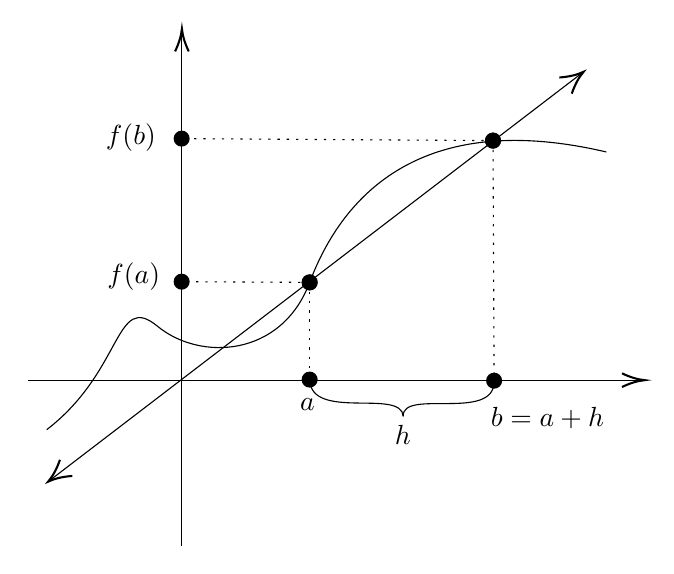
\begin{tikzpicture}[x=0.75pt,y=0.75pt,yscale=-1,xscale=1]
%uncomment if require: \path (0,441); %set diagram left start at 0, and has height of 441

%Straight Lines [id:da16102953695521127]
\draw    (163,221.33) -- (458,221.33) ;
\draw [shift={(460,221.33)}, rotate = 180] [color={rgb, 255:red, 0; green, 0; blue, 0 }  ][line width=0.75]    (10.93,-3.29) .. controls (6.95,-1.4) and (3.31,-0.3) .. (0,0) .. controls (3.31,0.3) and (6.95,1.4) .. (10.93,3.29)   ;
%Straight Lines [id:da9043079513680581]
\draw    (237.04,301) -- (237.04,54) ;
\draw [shift={(237.04,52)}, rotate = 90] [color={rgb, 255:red, 0; green, 0; blue, 0 }  ][line width=0.75]    (10.93,-3.29) .. controls (6.95,-1.4) and (3.31,-0.3) .. (0,0) .. controls (3.31,0.3) and (6.95,1.4) .. (10.93,3.29)   ;
%Curve Lines [id:da7565789477512073]
\draw    (171.9,245.19) .. controls (209.02,216.63) and (204.74,178.41) .. (225.27,195.34) .. controls (245.8,212.28) and (284.99,210.33) .. (298.59,174.22) .. controls (312.18,138.1) and (347.09,89.21) .. (441.52,111.39) ;
%Straight Lines [id:da9796385406474812]
\draw    (428.99,73.97) -- (174.17,269.02) ;
\draw [shift={(172.58,270.23)}, rotate = 322.57] [color={rgb, 255:red, 0; green, 0; blue, 0 }  ][line width=0.75]    (10.93,-4.9) .. controls (6.95,-2.3) and (3.31,-0.67) .. (0,0) .. controls (3.31,0.67) and (6.95,2.3) .. (10.93,4.9)   ;
\draw [shift={(430.57,72.75)}, rotate = 142.57] [color={rgb, 255:red, 0; green, 0; blue, 0 }  ][line width=0.75]    (10.93,-4.9) .. controls (6.95,-2.3) and (3.31,-0.67) .. (0,0) .. controls (3.31,0.67) and (6.95,2.3) .. (10.93,4.9)   ;
%Straight Lines [id:da4030910320179846]
\draw  [dash pattern={on 0.84pt off 2.51pt}]  (298.59,174.22) -- (298.59,221.05) ;
\draw [shift={(298.59,221.05)}, rotate = 90] [color={rgb, 255:red, 0; green, 0; blue, 0 }  ][fill={rgb, 255:red, 0; green, 0; blue, 0 }  ][line width=0.75]      (0, 0) circle [x radius= 3.35, y radius= 3.35]   ;
\draw [shift={(298.59,174.22)}, rotate = 90] [color={rgb, 255:red, 0; green, 0; blue, 0 }  ][fill={rgb, 255:red, 0; green, 0; blue, 0 }  ][line width=0.75]      (0, 0) circle [x radius= 3.35, y radius= 3.35]   ;
%Straight Lines [id:da14103701021608472]
\draw  [dash pattern={on 0.84pt off 2.51pt}]  (386.93,105.91) -- (387.46,221.58) ;
\draw [shift={(387.46,221.58)}, rotate = 89.74] [color={rgb, 255:red, 0; green, 0; blue, 0 }  ][fill={rgb, 255:red, 0; green, 0; blue, 0 }  ][line width=0.75]      (0, 0) circle [x radius= 3.35, y radius= 3.35]   ;
\draw [shift={(386.93,105.91)}, rotate = 89.74] [color={rgb, 255:red, 0; green, 0; blue, 0 }  ][fill={rgb, 255:red, 0; green, 0; blue, 0 }  ][line width=0.75]      (0, 0) circle [x radius= 3.35, y radius= 3.35]   ;
%Curve Lines [id:da47143485860977985]
\draw    (298.59,221.05) .. controls (299.18,241.14) and (342.98,225.16) .. (343.66,238.75) ;
%Curve Lines [id:da42610723931770456]
\draw    (387.46,221.58) .. controls (388.06,241.67) and (342.98,225.16) .. (343.66,238.75) ;
%Straight Lines [id:da3483526368480112]
\draw  [dash pattern={on 0.84pt off 2.51pt}]  (298.59,174.22) -- (236.91,173.88) ;
\draw [shift={(236.91,173.88)}, rotate = 180.32] [color={rgb, 255:red, 0; green, 0; blue, 0 }  ][fill={rgb, 255:red, 0; green, 0; blue, 0 }  ][line width=0.75]      (0, 0) circle [x radius= 3.35, y radius= 3.35]   ;
\draw [shift={(298.59,174.22)}, rotate = 180.32] [color={rgb, 255:red, 0; green, 0; blue, 0 }  ][fill={rgb, 255:red, 0; green, 0; blue, 0 }  ][line width=0.75]      (0, 0) circle [x radius= 3.35, y radius= 3.35]   ;
%Straight Lines [id:da4035786093366658]
\draw  [dash pattern={on 0.84pt off 2.51pt}]  (386.93,105.91) -- (236.91,104.95) ;
\draw [shift={(236.91,104.95)}, rotate = 180.37] [color={rgb, 255:red, 0; green, 0; blue, 0 }  ][fill={rgb, 255:red, 0; green, 0; blue, 0 }  ][line width=0.75]      (0, 0) circle [x radius= 3.35, y radius= 3.35]   ;
\draw [shift={(386.93,105.91)}, rotate = 180.37] [color={rgb, 255:red, 0; green, 0; blue, 0 }  ][fill={rgb, 255:red, 0; green, 0; blue, 0 }  ][line width=0.75]      (0, 0) circle [x radius= 3.35, y radius= 3.35]   ;

% Text Node
\draw (292.79,228.73) node [anchor=north west][inner sep=0.75pt]    {$a$};
% Text Node
\draw (384.59,233.05) node [anchor=north west][inner sep=0.75pt]    {$b=a+h$};
% Text Node
\draw (338.35,242.02) node [anchor=north west][inner sep=0.75pt]    {$h$};
% Text Node
\draw (199.88,163.44) node [anchor=north west][inner sep=0.75pt]    {$f( a)$};
% Text Node
\draw (199.19,96.46) node [anchor=north west][inner sep=0.75pt]    {$f( b)$};


\end{tikzpicture}

}

\vspace{4em}

\resizebox{3.25in}{!}{

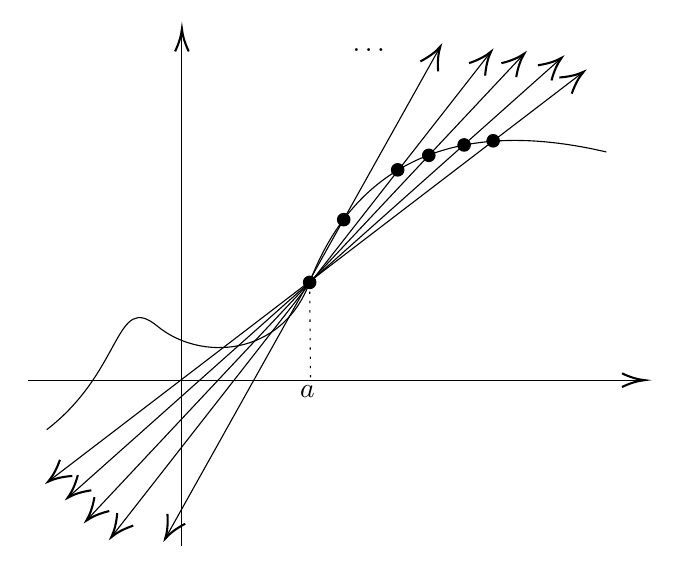
\begin{tikzpicture}[x=0.75pt,y=0.75pt,yscale=-1,xscale=1]
%uncomment if require: \path (0,441); %set diagram left start at 0, and has height of 441

%Straight Lines [id:da16102953695521127]
\draw    (163,221.33) -- (458,221.33) ;
\draw [shift={(460,221.33)}, rotate = 180] [color={rgb, 255:red, 0; green, 0; blue, 0 }  ][line width=0.75]    (10.93,-3.29) .. controls (6.95,-1.4) and (3.31,-0.3) .. (0,0) .. controls (3.31,0.3) and (6.95,1.4) .. (10.93,3.29)   ;
%Straight Lines [id:da9043079513680581]
\draw    (237.04,301) -- (237.04,54) ;
\draw [shift={(237.04,52)}, rotate = 90] [color={rgb, 255:red, 0; green, 0; blue, 0 }  ][line width=0.75]    (10.93,-3.29) .. controls (6.95,-1.4) and (3.31,-0.3) .. (0,0) .. controls (3.31,0.3) and (6.95,1.4) .. (10.93,3.29)   ;
%Curve Lines [id:da7565789477512073]
\draw    (171.9,245.19) .. controls (209.02,216.63) and (204.74,178.41) .. (225.27,195.34) .. controls (245.8,212.28) and (284.99,210.33) .. (298.59,174.22) .. controls (312.18,138.1) and (347.09,89.21) .. (441.52,111.39) ;
%Straight Lines [id:da9796385406474812]
\draw    (428.99,73.97) -- (174.17,269.02) ;
\draw [shift={(172.58,270.23)}, rotate = 322.57] [color={rgb, 255:red, 0; green, 0; blue, 0 }  ][line width=0.75]    (10.93,-4.9) .. controls (6.95,-2.3) and (3.31,-0.67) .. (0,0) .. controls (3.31,0.67) and (6.95,2.3) .. (10.93,4.9)   ;
\draw [shift={(430.57,72.75)}, rotate = 142.57] [color={rgb, 255:red, 0; green, 0; blue, 0 }  ][line width=0.75]    (10.93,-4.9) .. controls (6.95,-2.3) and (3.31,-0.67) .. (0,0) .. controls (3.31,0.67) and (6.95,2.3) .. (10.93,4.9)   ;
%Straight Lines [id:da1158565706067487]
\draw    (384.77,64.58) -- (204.23,295.42) ;
\draw [shift={(203,297)}, rotate = 308.03] [color={rgb, 255:red, 0; green, 0; blue, 0 }  ][line width=0.75]    (10.93,-4.9) .. controls (6.95,-2.3) and (3.31,-0.67) .. (0,0) .. controls (3.31,0.67) and (6.95,2.3) .. (10.93,4.9)   ;
\draw [shift={(386,63)}, rotate = 128.03] [color={rgb, 255:red, 0; green, 0; blue, 0 }  ][line width=0.75]    (10.93,-4.9) .. controls (6.95,-2.3) and (3.31,-0.67) .. (0,0) .. controls (3.31,0.67) and (6.95,2.3) .. (10.93,4.9)   ;
%Straight Lines [id:da7715304094905251]
\draw    (400.63,65.46) -- (192.37,287.54) ;
\draw [shift={(191,289)}, rotate = 313.16] [color={rgb, 255:red, 0; green, 0; blue, 0 }  ][line width=0.75]    (10.93,-4.9) .. controls (6.95,-2.3) and (3.31,-0.67) .. (0,0) .. controls (3.31,0.67) and (6.95,2.3) .. (10.93,4.9)   ;
\draw [shift={(402,64)}, rotate = 133.16] [color={rgb, 255:red, 0; green, 0; blue, 0 }  ][line width=0.75]    (10.93,-4.9) .. controls (6.95,-2.3) and (3.31,-0.67) .. (0,0) .. controls (3.31,0.67) and (6.95,2.3) .. (10.93,4.9)   ;
%Straight Lines [id:da44730990962603356]
\draw    (418.51,67.33) -- (183.49,276.67) ;
\draw [shift={(182,278)}, rotate = 318.31] [color={rgb, 255:red, 0; green, 0; blue, 0 }  ][line width=0.75]    (10.93,-4.9) .. controls (6.95,-2.3) and (3.31,-0.67) .. (0,0) .. controls (3.31,0.67) and (6.95,2.3) .. (10.93,4.9)   ;
\draw [shift={(420,66)}, rotate = 138.31] [color={rgb, 255:red, 0; green, 0; blue, 0 }  ][line width=0.75]    (10.93,-4.9) .. controls (6.95,-2.3) and (3.31,-0.67) .. (0,0) .. controls (3.31,0.67) and (6.95,2.3) .. (10.93,4.9)   ;
%Shape: Circle [id:dp8153494409622872]
\draw  [fill={rgb, 255:red, 0; green, 0; blue, 0 }  ,fill opacity=1 ] (384,106) .. controls (384,104.34) and (385.34,103) .. (387,103) .. controls (388.66,103) and (390,104.34) .. (390,106) .. controls (390,107.66) and (388.66,109) .. (387,109) .. controls (385.34,109) and (384,107.66) .. (384,106) -- cycle ;
%Shape: Circle [id:dp46038093787284295]
\draw  [fill={rgb, 255:red, 0; green, 0; blue, 0 }  ,fill opacity=1 ] (370,108) .. controls (370,106.34) and (371.34,105) .. (373,105) .. controls (374.66,105) and (376,106.34) .. (376,108) .. controls (376,109.66) and (374.66,111) .. (373,111) .. controls (371.34,111) and (370,109.66) .. (370,108) -- cycle ;
%Shape: Circle [id:dp190859565625209]
\draw  [fill={rgb, 255:red, 0; green, 0; blue, 0 }  ,fill opacity=1 ] (353,113) .. controls (353,111.34) and (354.34,110) .. (356,110) .. controls (357.66,110) and (359,111.34) .. (359,113) .. controls (359,114.66) and (357.66,116) .. (356,116) .. controls (354.34,116) and (353,114.66) .. (353,113) -- cycle ;
%Shape: Circle [id:dp3044800797092422]
\draw  [fill={rgb, 255:red, 0; green, 0; blue, 0 }  ,fill opacity=1 ] (338,120) .. controls (338,118.34) and (339.34,117) .. (341,117) .. controls (342.66,117) and (344,118.34) .. (344,120) .. controls (344,121.66) and (342.66,123) .. (341,123) .. controls (339.34,123) and (338,121.66) .. (338,120) -- cycle ;
%Shape: Circle [id:dp7651386739199335]
\draw  [fill={rgb, 255:red, 0; green, 0; blue, 0 }  ,fill opacity=1 ] (295.59,174.22) .. controls (295.59,172.56) and (296.93,171.22) .. (298.59,171.22) .. controls (300.24,171.22) and (301.59,172.56) .. (301.59,174.22) .. controls (301.59,175.87) and (300.24,177.22) .. (298.59,177.22) .. controls (296.93,177.22) and (295.59,175.87) .. (295.59,174.22) -- cycle ;
%Straight Lines [id:da21925282533113744]
\draw  [dash pattern={on 0.84pt off 2.51pt}]  (298.59,174.22) -- (299,221) ;
%Straight Lines [id:da4492754198498514]
\draw    (360.57,62.35) -- (229.98,295.92) ;
\draw [shift={(229,297.67)}, rotate = 299.21] [color={rgb, 255:red, 0; green, 0; blue, 0 }  ][line width=0.75]    (10.93,-4.9) .. controls (6.95,-2.3) and (3.31,-0.67) .. (0,0) .. controls (3.31,0.67) and (6.95,2.3) .. (10.93,4.9)   ;
\draw [shift={(361.54,60.61)}, rotate = 119.21] [color={rgb, 255:red, 0; green, 0; blue, 0 }  ][line width=0.75]    (10.93,-4.9) .. controls (6.95,-2.3) and (3.31,-0.67) .. (0,0) .. controls (3.31,0.67) and (6.95,2.3) .. (10.93,4.9)   ;
%Shape: Circle [id:dp18797969215530874]
\draw  [fill={rgb, 255:red, 0; green, 0; blue, 0 }  ,fill opacity=1 ] (312,144) .. controls (312,142.34) and (313.34,141) .. (315,141) .. controls (316.66,141) and (318,142.34) .. (318,144) .. controls (318,145.66) and (316.66,147) .. (315,147) .. controls (313.34,147) and (312,145.66) .. (312,144) -- cycle ;

% Text Node
\draw (292.79,222.73) node [anchor=north west][inner sep=0.75pt]    {$a$};
% Text Node
\draw (318,60.4) node [anchor=north west][inner sep=0.75pt]    {$\dotsc $};


\end{tikzpicture}

}

\end{multicols}


You'll notice that the tangent line captures some \textit{local information} about $f$ at $a$. In other words, it is a good approximation of $f$ at $a$; that is, $f$ and its tangent line are ``similar'' at $a$. Intuitively, you should think about the tangent line at $a$ to be the line that ``hugs $f$ the best at $a$.''

Note that this definition of the derivative only makes sense if $f$ is defined on an open interval containing $a$. We can view the derivative as a function, and write $[f(x)]'$ or $f'(x)$. The derivative of $f'(x)$ is called the \textbf{second derivative} and is denoted $f''(x)$. In general, the $n$th derivative $f^{(n)}(x)$ is defined to be the derivative of $f^{(n-1)}(x)$.

\subsection{The Two Part ``Program'' for Finding Derivatives}

So now we have a goal: find derivatives of functions. The problem is that the limit definition is difficult to use (that pesky $h\to 0$ in the denominator). So instead, we will do the following two steps (let $a$ be a real number and $f$ and $g$ be functions):
\begin{enumerate}
\item rules to break functions up and reassemble

\begin{center}
\def\arraystretch{1.5}
\begin{tabular}{@{}ll@{}}
\toprule[0.4mm]
\textbf{The Scalar Multiple Rule} & $[af]' = af'$. \\
\textbf{The Sum Rule} & $[f + g]' = f' + g'$ \\
\textbf{The Product Rule} & $[fg]' = f'g + fg'$ \\
\textbf{The Quotient Rule} & $\left[\frac{f}{g}\right]' = \frac{f'g - fg'}{g^2}$ \\
\textbf{The Chain Rule} & $[f(g(x))]' = f'(g(x))g'(x)$ \\
\textbf{The Inverse Rule} & $[f^{-1}(x)]' = \frac{1}{f'(f^{-1}(x))}$ \\
\bottomrule[0.4mm]
\end{tabular}
\end{center}

\item find derivatives of ``basic'' functions:

\end{enumerate}


\begin{center}
\def\arraystretch{1.5}
\begin{tabular}{@{}ll@{}}
\toprule[0.4mm]
\textbf{The Constant Rule}     & $[a]' = 0$ \\
\textbf{The Power Rule}        & $[x^a]' = ax^{a-1}$ \\
\textbf{Trig Rules}  & $[\sin(x)]' = \cos(x)$ and $[\cos(x)]' = -\sin(x)$ \\
\textbf{Exponential Rules} & $[a^x]' = \ln(a)a^x$ \\
\textbf{Logarithmic Rules} & $[\log_a(x)]' = \frac{1}{x\ln(a)}$ \\
\bottomrule[0.4mm]
\end{tabular}
\end{center}


Most of the time, you will be able to find the derivatives using a combination of these rules. For instance, the derivatives of the other 4 trig functions can be found using the quotient rule and the derivatives of $\sin$ and $\cos$:
$$[\tan(x)]' = \sec^2(x)
\quad\quad\quad\quad\quad
[\sec(x)]' = \sec(x)\tan(x)$$

$$[\cot(x)]' = -\csc^2(x)
\quad\quad\quad\quad\quad
[\csc(x)]' = -\csc(x)\cot(x)$$
\mar{Try to find the pattern with these four derivatives.}


\subsection{Implicit Differentiation}

We'll refer to the set of points that satisfy an equation of two variables as a \textbf{curve in the plane}. Some examples you might have seen before are circles and ellipses. The circle with center $(h,k)$ and radius $r$ is the set of points $(x,y)$ in the plane that satisfy the equation
$$(x-h)^2+(y-k)^2=r^2.$$
\mar{Look up the similar equation for an ellipse and write it down here.}

In general, curves are not functions (they might not pass the vertical line test), but they can still have tangent lines, so we should be able to describe their slope at a point. We do this by ``zooming in'' on a point of the curve, and forgetting about the other parts of the curve. Now (locally), it looks like a function, so we can treat the $y$ variable as a function of $x$. This process is called ``implicit'' differentiation, and consists of two steps:
\begin{enumerate}
\item differentiate both sides of the equation (keeping in mind that since $y$ is a function of $x$, the derivative of $f(y)$ is $f'(y)\cdot y'$ by the chain rule).
\item solve for $y'$.
\end{enumerate}

Other notation is sometimes used: if $y=f(x)$, $\frac{dy}{dx}=\frac{d}{dx}[f(x)]$ is the derivative of $f$, and $\frac{d^ny}{dx^n}=\frac{d^n}{dx^n}[f(x)]$ is the $n$th derivative of $f$.

When you solve for $y'$, it is possible that the expression will consist of both $y$ and $x$ variables. That is because the formula for $y'$ is not a function of just $x$, it is a function of both $x$ and $y$!

Let's do an example:
\begin{itemize}
\item The curve of points satisfying the equation $y^{3}=x^{2}-xy-1$ is not a function, since it does not pass the vertical line test: both $(-1,-1)$ and $(-1,1)$ are solutions. However, we can still find the derivative at each point on this curve! Start by taking the ($x$) derivative of both sides.

On the left, the $x$ derivative of $y^3$ is $3y^2y'$, by the power rule (and the chain rule). The derivative of $x^2$ is $2x$, the derivative of $xy$ is $y+xy'$ by the product rule (and chain rule), and the derivative of $1$ is 0, of course. Comparing the derivatives of each side of the equation, we get
$$3y^2y'=2x-(y+xy'),$$
so solving for $y'$,
$$y'=\frac{2x-y}{3y^2+x}.$$
At $(-1,1)$, $y'=\frac{-3}{2}$, and at $(-1,-1)$, $y'=\frac{-1}{2}$. The tangent line to the curve at the point $(-1,1)$ is $y=\frac{-3}{2}(x+1)+1$

\end{itemize}


\subsection{Logarithmic Differentiation}

Sometimes you will be faced with a function whose formula includes an expression involving $x$ raised to a power that also involves $x$. Finding the derivative of such a function has a specific procedure:
\begin{strat}[Logarithmic Differentiation]
Suppose $y=f(x)^{g(x)}$ and we want to find $y'$. First apply the $\ln$ function to both sides of the equation and use the log property $\ln(a^b)=b\ln(a)$:
$$\ln(y)=\ln(f(x)^{g(x)})=g(x)\ln(f(x)).$$
Then implicit differentiation yields
$$\frac{1}{y}y'=g'(x)\ln(f(x))+g(x)\frac{f'(x)}{f(x)},$$
and solving for $y'$ and substituting $y=f(x)^{g(x)}$ we get
$$y'=f(x)^{g(x)}\left(g'(x)\ln(f(x))+g(x)\frac{f'(x)}{f(x)}\right).$$
\end{strat}

Here are some examples:
\begin{itemize}
\item $[x^x]'=x^x(\ln(x)+1)=\ln(x^{x^x})+x^x$. (Here $f(x)=g(x)=x$).
\item $[\sin(x)^x]'=\sin(x)^x(\ln(\sin(x))+x\cot(x))$. (Here $f(x)=\sin(x)$ and $g(x)=x$). \mar{Work these examples out.}
\end{itemize}

I don't recommend that you memorize the formula for $[f(x)^{g(x)}]'$. Instead, remember the procedure and re-create when you need it.


\subsection{Using The Inverse Rule}

When we want to find the derivative of an inverse of a function $f$, the inverse rule tells us that
$$[f^{-1}(x)]'=\frac{1}{f'(f^{-1}(x))},$$
but how is this helpful? It is actually very easy to see why this rule is true:
\begin{align*}
         & f(f^{-1}(x)) = x & & \text{(definition of inverse)}\\
\implies & f'(f^{-1}(x))[f^{-1}(x)]'=1 & &\text{(chain rule)}\\
\implies & [f^{-1}(x)]' = \frac{1}{f'(y)} & & \text{(solve for $[f^{-1}(x)]'$)}\\
\implies & [f^{-1}(x)]' =\frac{1}{f'(f^{-1}(x))} & & \text{(substitute)}
\end{align*}

Let's use this rule to find the derivative of inverse trig functions:
\begin{itemize}
\item The rule says that $[\sin^{-1}(x)]'=\frac{1}{\cos(\sin^{-1}(x))}$, but we should be able to simplify this expression using the unit circle.
\begin{figure}[h!]
\centering
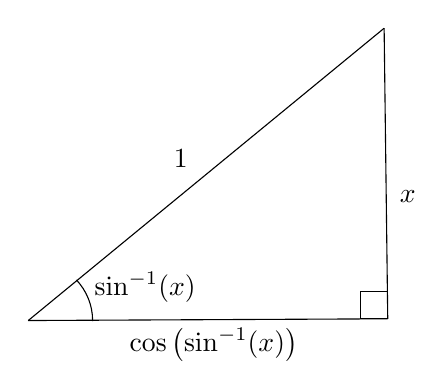
\begin{tikzpicture}[x=0.75pt,y=0.75pt,yscale=-1,xscale=1]
%uncomment if require: \path (0,479); %set diagram left start at 0, and has height of 479

%Straight Lines [id:da021711983663396772]
\draw    (216.29,266.83) -- (389.5,266) ;
%Straight Lines [id:da1995895124000051]
\draw    (387.76,126) -- (216.29,266.83) ;
%Shape: Arc [id:dp31180800912218465]
\draw  [draw opacity=0] (239.51,247.26) .. controls (244.36,252.47) and (247.3,259.32) .. (247.3,266.83) .. controls (247.3,266.94) and (247.3,267.05) .. (247.3,267.16) -- (216.29,266.83) -- cycle ; \draw   (239.51,247.26) .. controls (244.36,252.47) and (247.3,259.32) .. (247.3,266.83) .. controls (247.3,266.94) and (247.3,267.05) .. (247.3,267.16) ;
%Straight Lines [id:da12311387270862384]
\draw    (387.76,126) -- (389.5,266) ;
%Shape: Square [id:dp5026691075905794]
\draw   (376.5,253) -- (389.5,253) -- (389.5,266) -- (376.5,266) -- cycle ;

% Text Node
\draw (247,242) node [anchor=north west][inner sep=0.75pt]    {$\sin^{-1}( x)$};
% Text Node
\draw (263.9,269) node [anchor=north west][inner sep=0.75pt]   [align=left] {$\displaystyle \cos\left(\sin^{-1}(x)\right)$};
% Text Node
\draw (285.15,183.17) node [anchor=north west][inner sep=0.75pt]   [align=left] {$\displaystyle 1$};
% Text Node
\draw (394.13,203) node [anchor=north west][inner sep=0.75pt]   [align=left] {$\displaystyle x$};


\end{tikzpicture}
\end{figure}

\mar{Argue this using the Pythagorean identitiy ($\sin^2\theta+\cos^2\theta = 1$) instead.}

if a (non-right) angle of a right triangle (with hypotenuse 1) is $\sin^{-1}(x)$, the leg opposite $\sin^{-1}(x)$ has length $x$. Then $\cos(\sin^{-1}(x))$ is the length of the other leg of the triangle, so $\cos(\sin^{-1}(x))=\sqrt{1-x^2}$ by the Pythagorean theorem. Therefore,
$$[\sin^{-1}(x)]'=\frac{1}{\cos(\sin^{-1}(x))}=\frac{1}{\sqrt{1-x^2}}.$$\item The derivatives of the other inverse trig functions are
\mar{Figure these equations out by yourself using the same method as for $\sin^{-1}$. Hint: refer to Figure \ref{6trig}}
\begin{align*}
[\cos^{-1}(x)]' & =\frac{-1}{\sqrt{1-x^2}} \\
[\csc^{-1}(x)]' & =\frac{-1}{|x|\sqrt{x^2-1}} \\
[\sec^{-1}(x)]' & =\frac{1}{|x|\sqrt{x^2-1}} \\
[\tan^{-1}(x)]' & =\frac{1}{1+x^2} \\
[\cot^{-1}(x)]' & =\frac{-1}{1+x^2}
\end{align*}
\end{itemize}

% \subsection{Summary}

% \begin{strat}[Finding the Derivative of a Function]
% \begin{enumerate}
% \item
% \end{enumerate}

% \end{strat}



\newpage

\section{Applications of Derivatives}


\subsection{Linear Approximation}

This first application of derivatives is nothing too new! We first described the tangent line of a function $f$ as the line that ``hugs $f$ the best at $a$'' and now we are going to take of advantage of that fact.

The main idea is that if we have a function $f$ and we know $f(a)$ and $f'(a)$ for some $a$, then we can use the tangent line of $f$ at $a$ to estimate values of a function near $a$. That is, if $a\approx b$, then
$$f(b)\approx f(a)+f'(a)(b-a).$$\mar{When is this approximation an overestimate? Underestimate?}
The right side of this approximation is exactly the tangent line of $f$ at $a$, evaluated at $b$.

\begin{figure}[h!]
\centering
\fbox{
\tikzset{every picture/.style={line width=0.75pt}} %set default line width to 0.75pt
\begin{tikzpicture}[x=0.75pt,y=0.75pt,yscale=-1,xscale=1]
%uncomment if require: \path (0,300); %set diagram left start at 0, and has height of 300

%Straight Lines [id:da290856484859926]
\draw    (189,231) -- (547,231.2) ;
%Straight Lines [id:da7357645784694884]
\draw    (210,10) -- (210,272.2) ;
%Curve Lines [id:da5579528590630709]
\draw    (210,231) .. controls (396,38) and (419,51) .. (540,226) ;
%Straight Lines [id:da4409257410178691]
\draw    (205,170) -- (521,27.2) ;
%Straight Lines [id:da8838372850567859]
\draw  [dash pattern={on 0.84pt off 2.51pt}]  (363,98.6) -- (363,232.2) ;
%Straight Lines [id:da5277023069496161]
\draw  [dash pattern={on 0.84pt off 2.51pt}]  (407,79) -- (406,231) ;
%Straight Lines [id:da42915482489298684]
\draw  [dash pattern={on 0.84pt off 2.51pt}]  (407,91.6) -- (210,93) ;
%Straight Lines [id:da3902230699344138]
\draw  [dash pattern={on 0.84pt off 2.51pt}]  (407,79) -- (210.5,79) ;
%Straight Lines [id:da5116345937274027]
\draw  [dash pattern={on 0.84pt off 2.51pt}]  (363,98.6) -- (210,100) ;
%Curve Lines [id:da33167985133818645]
\draw    (169.75,48) .. controls (191.42,48) and (175.98,78.08) .. (208.96,78.98) ;
\draw [shift={(210.5,79)}, rotate = 180] [color={rgb, 255:red, 0; green, 0; blue, 0 }  ][line width=0.75]    (10.93,-3.29) .. controls (6.95,-1.4) and (3.31,-0.3) .. (0,0) .. controls (3.31,0.3) and (6.95,1.4) .. (10.93,3.29)   ;
%Curve Lines [id:da3661693241843025]
\draw    (170.75,131) .. controls (193.16,131) and (175.55,100.92) .. (208.46,100.02) ;
\draw [shift={(210,100)}, rotate = 180] [color={rgb, 255:red, 0; green, 0; blue, 0 }  ][line width=0.75]    (10.93,-3.29) .. controls (6.95,-1.4) and (3.31,-0.3) .. (0,0) .. controls (3.31,0.3) and (6.95,1.4) .. (10.93,3.29)   ;
%Straight Lines [id:da2376462542003681]
\draw    (170.75,93) -- (208,93) ;
\draw [shift={(210,93)}, rotate = 180] [color={rgb, 255:red, 0; green, 0; blue, 0 }  ][line width=0.75]    (10.93,-3.29) .. controls (6.95,-1.4) and (3.31,-0.3) .. (0,0) .. controls (3.31,0.3) and (6.95,1.4) .. (10.93,3.29)   ;

% Text Node
\draw (357,235) node [anchor=north west][inner sep=0.75pt]    {$a$};
% Text Node
\draw (137,120) node [anchor=north west][inner sep=0.75pt]    {$f(a)$};
% Text Node
\draw (401,235.4) node [anchor=north west][inner sep=0.75pt]    {$b$};
% Text Node
\draw (140,85) node [anchor=north west][inner sep=0.75pt]    {$f( b)$};
% Text Node
\draw (125,40) node [anchor=north west][inner sep=0.75pt]    {$\approx f( b)$};


\end{tikzpicture}
}
\caption{Linear Approximation}
\end{figure}

Let's pretend we don't have a calculator, and try to estimate $\sqrt{4.1}$. In this case $f(x)=\sqrt{x}$, and we should set $a=4$, since $4.1\approx 4$ and we can figure out $f(4)$ and $f'(4)$. By the power rule, $f'(x)=\frac{1}{2}x^{-1/2}$, so $f'(4)=\frac12(4^{-1/2})=\frac14$, and of course $f(4)=\sqrt{4}=2$. Using the formula above,
$$\sqrt{4.1}=f(4.1)\approx f(4)+f'(4)(4.1-4)=2+\frac14(0.1)=2.025.$$
If we check a calculator for a better approximation, we find that
$$\sqrt{4.1}\approx 2.02484567313,$$
so we weren't that far off! \mar{Estimate $\sqrt{3.9}$ and compare to the actual value.}

\subsection{L'H\^opital's Rule}

L'H\^opital's Rule is a way to easily tackle some of those limit problems that were in an indeterminate form, namely $\frac{0}{0}$ and $\frac{\infty}{\infty}$.

\begin{thm}
If $\displaystyle \lim_{x\to a} f(x)= \lim_{x\to a} g(x)= 0$ or $\infty$, then
$$\lim_{x\to a}\frac{f(x)}{g(x)}=\lim_{x\to a}\frac{f'(x)}{g'(x)},$$
as long as all of these limits are defined.
\end{thm}

What this means for you: if you are trying to take the limit of a rational function and after plugging in you get $\frac{0}{0}$ or $\frac{\infty}{\infty}$, then take the derivative of the numerator and the denominator, and try to evaluate the limit again.

It is possible that one use of L'H\^optial's rule won't be enough: you may have to use it multiple times. Here are some examples:
\begin{itemize}
\item $\displaystyle \lim_{x\to 0}\frac{\sin(x)}{x}\overset{\text{LH}}{=}\lim_{x\to 0}\frac{\cos(x)}{1}=1.$
\item $\displaystyle \lim_{x\to \infty}\frac{3x^2+1}{4x^2+3x}\overset{\text{LH}}{=}\lim_{x\to\infty}\frac{6x}{8x+3}\overset{\text{LH}}{=}\lim_{x\to\infty}\frac{6}{8}=\frac{3}{4}$.
\end{itemize}

Sometimes you will encounter an indeterminant form that is not $\frac00$ or $\frac\infty\infty$, and in these cases, we can transform it into the form $\frac00$ or $\frac\infty\infty$ and then use L'H\^optial's rule. Here are some illustriative examples:

\begin{itemize}

\item
$\displaystyle \lim_{x\to1} \frac{1}{x-1} - \frac{1}{\ln(x)}
= \lim_{x\to1} \frac{\ln\left(x\right)-x+1}{(x-1)\ln\left(x\right)}
\overset{\text{LH}}{=} \lim_{x\to1}\frac{{1}/{x}-1}{\ln\left(x\right)+1-\frac{1}{x}}$\\
\phantom{} \hspace{1.01in}$\overset{\text{LH}}{=}\lim_{x\to1} \frac{-{1}/{x^{2}}}{{1}/{x}+{1}/{x^{2}}}
=-\frac12$.

\item
$\displaystyle \lim_{x\to 0^+} x\ln(x) =\lim_{x\to 0^+} \frac{\ln(x)}{1/x} \overset{\text{LH}}{=}\lim_{x\to0^+}\frac{1/x}{-1/x^2}=\lim_{x\to0^+}-x=0$.

\item $\displaystyle\lim_{x\to 0^+} x^x =\lim_{x\to0^+}e^{\ln(x^x)}=e^{\displaystyle\lim_{x\to0^+}\ln(x^x)}=e^{\displaystyle\lim_{x\to 0^+}x\ln(x)} = e^0 = 1.$


\mar{Label each of these examples with original and trasnsformed type of indeterminant forms they demonstrate.}


% \item $\displaystyle\lim_{x\to\infty}\left(1+\frac{1}{x}\right)^x = e^{\displaystyle\lim_{x\to\infty}\textstyle\frac{\ln\left(1+\frac{1}{x}\right)}{1/x}}\overset{\text{LH}}{=}e^{\displaystyle\lim_{x\to\infty}\textstyle \frac{(-1/x^2)/(1+1/x)}{-1/x^2}}=e^{\displaystyle\lim_{x\to\infty}\textstyle \frac{1}{1+1/x}}= e$.

% \item ($\infty ^ 0$)

\end{itemize}





\subsection{Kinematics}

Kinematics is the study of motion. In this section, we'll concern ourselves with only one basic situation: an object moving in a straight path (only forwards and backwards).

Suppose the position of an object at time $t$ is given by $x(t)$. The object's \textbf{velocity} at time $t$ is given by $$v(t)=x'(t)$$ since velocity is the rate at which position is changing. Similarly, the object's \textbf{acceleration} at time $t$ is given by $$a(t)=v'(t)=x''(t),$$ since acceleration is the rate at which velocity is changing.

How do we interpret these quantities? One way is to think about \textbf{speed}, which is the absolute value of velocity. In other words, if you are moving backward at 2 m/s, then your velocity is $-$2 m/s and you speed is 2 m/s, but if you are moving forward at the speed 2 m/s, then your speed and velocity are both 2 m/s.


\mar{What is an example of a position function whose velocity is positive?}


\subsection{Related Rates}

As we saw in kinematics, the time-derivative of a function tells us the rate at which the function is changing. So, if we have two related quantities $A$ and $B$ that are changing over time, we can find the rate at which $A$ is changing at time $T$ if we know the rate at which $B$ is changing at time $T$.

Note: sometimes the following different notations are used for the time derivative of $A$ at time $T$:

$$A'(T)\quad =\quad \frac{dA}{dt}\biggm\lvert_{t=T}\quad=\quad\dot{A}(T)$$

Here is the general problem-solving strategy:

\begin{strat}[Related Rates]
\begin{enumerate}[leftmargin=1em]
\item Draw a picture.
\item Label the relevant quantities (including $A$ and $B$).
\item Find an equation that relates $A$ and $B$ (and nothing else).
\item Implicitly differentiate the equation with respect to time $t$. (Remember that $A$ and $B$ are functions of $t$, so use the chain rule!)
\item Solve for $A'(t)$ in terms of $A(t)$, $B(t)$, and $B'(t)$
\item Plug in $t=T$.
\end{enumerate}
\end{strat}



\subsection{Qualities of Graphs}

In this section we will understand how derivatives tell us qualitative information about of graphs of functions. To start,
$$f \text{ is }
\begin{cases}\text{increasing at }x &\text{ if } f'(x)>0 \\ \text{decreasing at }x &\text{ if } f'(x)<0\end{cases}
$$
and
$$
f \text{ is }\begin{cases}\text{concave up at }x &\text{ if } f''(x)>0 \\ \text{concave down at }x &\text{ if } f''(x)<0.\end{cases}
$$
You already know what \textbf{increasing} and \textbf{decreasing} mean. The graph of a function that is \textbf{concave up at $x$} looks like a bowl near $x$, and the graph of a function that is \textbf{concave down at $x$} looks like a hill near $x$. Points on a graph where concavity changes (from up to down, or down to up) are called \textbf{inflection points}. \mar{Draw a sketch of an inflection point.}

\begin{thm}[The Mean Value Theorem]
If $f$ is continuous on $[a,b]$ and differentiable on $(a,b)$, then there is some $c\in (a,b)$ for which $f'(c)=\frac{f(b)-f(a)}{b-a}$.
\end{thm}

In plain English, the mean value theorem says that the average value of the slope on an interval is always attained on that interval.










% \textsc{In progress.}

% It is helpful to be able to look at a graph of a function and understand what it means for its first and second derivative. The table below summarizes:

% \begin{center}
% \def\arraystretch{1.3}
% \begin{tabular}{@{}lll@{}}
% \toprule[0.4mm]
% $f$ & $f'$ & $f''$ \\
% \midrule
% increasing & positive & \\
% constant & 0 & \\
% decreasing & negative & \\
% \midrule
% concave up & increasing & positive \\
% linear & constant & 0 \\
% concave down & decreasing & negative \\
% \bottomrule[0.4mm]

% Inflection point & constant & 0 \\ \hline
% local extrema & 0 & \\ \hline
% \hline

% \end{tabular}
% \end{center}



\subsection{Extremal Points}

\noindent A function $f$ has a
$$\textbf{local} \begin{cases}\textbf{maximum}\\\textbf{minimum}\end{cases}\text{at }a \text{ if }\begin{cases}f(a)\geq f(x)\\f(a)\leq f(x)\end{cases} \text{for all $x$ in some interval $I\ni a$};$$

$$\textbf{global} \begin{cases}\textbf{maximum}\\\textbf{minimum}\end{cases}\text{at }a \text{ if }\begin{cases}f(a)\geq f(x)\\f(a)\leq f(x)\end{cases} \text{for all $x$ in the domain of $f$}.$$
Any such point is called an \textbf{extremal point} of $f$.

Global maximum \textit{values} are unique, but points at which they occur might not be. For example, $\sin(x)$ has global maximum value of $1$, even though this value occurs infinitely many times on the domain of $\sin(x)$. All global extremal points are local extremal points.


The point $a$ is called a \textbf{critical point} of $f$ if $f'(a)=0$ or $f$ is not differentiable at $a$ ($f'(a)$ doesn't exist). The following theorem tells us how find extremal points using critical points.

\begin{thm}
If $a$ is an extremal point of $f$, $a$ is a critical point of $f$.
\end{thm}

\noindent WARNING: The converse is not true! (i.e. not all critical points are extremal!)\mar{Name and draw a function with a non-extremal critical point.}

\begin{thm}[First Derivative Test]
Suppose $a$ is a critical point of $f$.
$$\text{If $f'$ } \begin{cases}
\text{changes from $(+)$ to $(-)$}\\
\text{changes from $(-)$ to $(+)$}\\
\text{doesn't change sign}\\
\end{cases}
\text{at $a$, then $a$ is}
\begin{cases}
\text{a local maximum of $f$}.\\
\text{a local minimum of $f$}.\\
\text{not a extremal point}.\\
\end{cases}$$
\end{thm}


\begin{thm}[Second Derivative Test]
Suppose $f'(a)=0$ and $f''$ is continuous at $a$.
$$\text{If } \begin{cases}
f''(a)>0\\
f''(a)<0
\end{cases}
\text{then $a$ is a}
\begin{cases}
\text{local minimum}\\
\text{local maximum}
\end{cases} \text{of $f$}.$$
\end{thm}


\begin{strat}[Finding Extremal Points]
\begin{enumerate}[leftmargin=1em]
\item Solve $f'(x)=0$ for $x$.
\item Find other critical points (points of non-differentiability such as endpoints of the domain, cusps, peaks, and points of discontinuity).
\item If you are looking for \textit{local} extremal points, use the first or second derivative tests as necessary to classify points the critical points you found.
\item If you are looking for \textit{global} extremal points, evaluate $f$ at each critical points to find the largest and smallest.
\end{enumerate}
\end{strat}


\subsection{Optimization}

``Optimization''-style questions will ask you to optimize (maximize or minimize) a certain quantity $A$ under specified constraints. The constraints will still allow one variable $x$ of change. This means you will need to find the value of $x$ for which $A$ is maximal or minimal. 

The strategy for optimization problems is very similar to the strategy for related rates, but uses the theory of extremal points from the previous section.

\begin{strat}[Optimization]
\begin{enumerate}[leftmargin=1em]
\item Draw a picture.
\item Label the relevant quantities.
\item Find an equation for the quantity that you want to optimize $A$ in terms of the thing that you can change $x$ (and note the domain of $A$).
\item Find the extremal points of $A$.
\end{enumerate}
\end{strat}


\subsection{Newton's Method for Finding Roots}

Imagine that you have an function $f$ and you want to find the zeros (or roots) of $f$. That is, you want to find the values of $x$ such that $f(x)=0$. \textbf{Newton's Method} is a computational algorithm that can sometimes be used to approximate such a value. First, we'll describe the algorithm, and then we'll show how to do use your TI calculator to implement it.

Imagine that $x_0$ is an initial guess of a root of the function $f$. If we can take the derivative of $f$, then we know that the tangent line of $f$ at $x_0$ is
$$y-f(x_0)=f'(x_0)(x-x_0)$$
and so we find (setting $y=0$ and solving for $x$) this tangent line intersects the $x$-axis at the point $(x_1,0)$, where
$$x_1=x_0-\frac{f(x_0)}{f'(x_0)}.$$
We continue this, setting
$$x_2=x_1-\frac{f(x_1)}{f'(x_1)},$$
and so on:
$$x_{n+1}=x_n-\frac{f(x_n)}{f'(x_n)}.$$

In many cases, this sequence of numbers should approach a zero of $f$. Here is the intuitive reason why: (1) if $x_n$ is not a zero of $f$, then $x_{n+1}$ moves in the direction of a zero, and (2) if $x_n$ is a zero of $f$, then $x_{n+1}=x_n$.

The second point is obvious, but let's look into the first point. If $f(x_n)$ is not 0, then we have two cases:
\begin{itemize}
\item $x_n<x_{n+1}$ (move to the right).  Algebraically, this occurs exactly when $f(x_n)$ and $f'(x_n)$ have opposite sign (when $f$ is increasing below the $x$-axis, or decreasing above the $x$-axis). \mar{Draw a picture showing the four cases.}
\item $x_{n+1}<x_n$ (move to the left). Similarly, this occurs exactly when $f(x_n)$ and $f'(x_n)$ have the same sign (when $f$ is increasing above the $x$-axis, or decreasing below the $x$-axis).
\end{itemize}

Seems reasonable, right? In either case we try to move in the direction of  a root.

Now, how do we use Newton's method? Get out your TI calculator, and type the function $f$ into \texttt{Y$_\text{1}$=}, and $f'$ into \texttt{Y$_\text{2}$=}. Then return to the main calculator screen and type
\begin{center}
\texttt{0 \MVRightarrow \ A}
\end{center}
(or replace the 0 with a different initial guess $x_0$) and click \texttt{ENTER}. Then type
\begin{center}
\texttt{A - Y$_\text{1}$(A)/Y$_\text{2}$(A) \MVRightarrow \ A}
\end{center}
and click \texttt{ENTER}. The variable \texttt{A} is now set as $x_1$, and this value should be displayed. Click \texttt{ENTER} again and \texttt{A} is now $x_2$. Continue clicking \texttt{ENTER} to find $x_n$ for higher $n$ (clicking 100 times will show you $x_{100}$).

Although Newton's method is generally an easy algorithm to implement and use, it does not always work.\mar{Consider $f(x)=x^3$ and try to use Newtons method to detect the root $0$ with the initial guess $x_0=1$.}



\newpage
\part{Integration and Applications}
\section{The Definite Integral}

For reasons that will not be immediately obvious, integration is opposite differentiation on the `calculus coin.'

\subsection{The Definite Integral}

The \textbf{definite integral of $f$ on $(a,b)$} is written 
$$\int_a^bf(x)\ dx$$
and is defined to be the \textit{signed} area between the graph of $f$ and the $x$-axis (if such a quantity exists). \mar{When might this quantity not exist?}

\begin{figure}[h!]
\centering
\fbox{
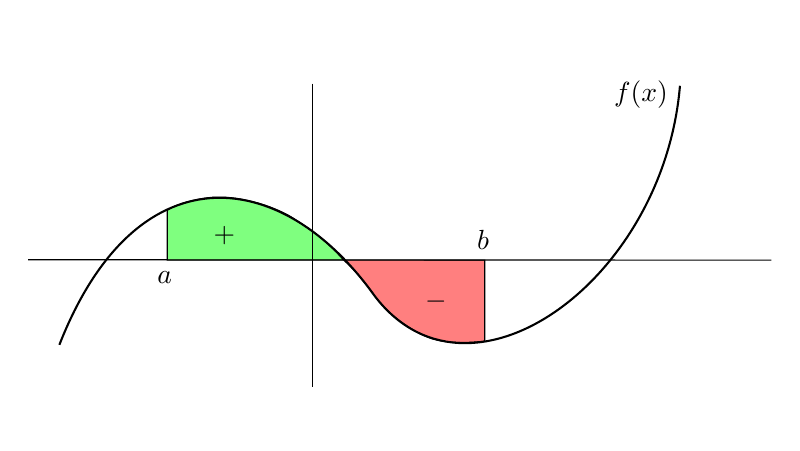
\begin{tikzpicture}[x=0.75pt,y=0.75pt,yscale=-1,xscale=1]
\path (150,50);

%Shape: Polygon Curved [id:ds707129257032501] 
\draw  [fill={rgb, 255:red, 0; green, 255; blue, 0 }  ,fill opacity=0.5 ] (217,162) .. controls (217,162) and (217,138) .. (217,138) .. controls (217,138) and (222,134) .. (236,132) .. controls (250,130) and (269,136) .. (278,142) .. controls (287,148) and (288.41,149.01) .. (293,153) .. controls (297.59,156.99) and (302,162) .. (302,162) .. controls (302,162) and (217,162) .. (217,162) -- cycle ;
%Shape: Polygon Curved [id:ds12696670726714787] 
\draw  [fill={rgb, 255:red, 255; green, 0; blue, 0 }  ,fill opacity=0.5 ] (370,162) .. controls (370,162) and (370,201) .. (370,201) .. controls (370,201) and (355,203) .. (345,200) .. controls (335,197) and (322,187) .. (316,178) .. controls (310,169) and (302,162) .. (302,162) .. controls (302,162) and (370,162) .. (370,162) -- cycle ;
%Straight Lines [id:da2259128899132099] 
\draw    (150,161.8) -- (508,162) ;
%Straight Lines [id:da519801972092973] 
\draw    (287,77) -- (287,223) ;
%Curve Lines [id:da2537963372820191] 
\draw [line width=0.75]    (165,202.8) .. controls (201.6,109.5) and (271,116) .. (316,178) .. controls (361,240) and (456,173) .. (464,78) ;
%Straight Lines [id:da8858936847665124] 
\draw    (217,138) -- (217,162) ;
%Straight Lines [id:da05784827822991523] 
\draw    (370,162) -- (370,201) ;

% Text Node
\draw (211,166.4) node [anchor=north west][inner sep=0.75pt]    {$a$};
% Text Node
\draw (365,146.4) node [anchor=north west][inner sep=0.75pt]    {$b$};
% Text Node
\draw (431,74.4) node [anchor=north west][inner sep=0.75pt]    {$f( x)$};
% Text Node
\draw (238,144.4) node [anchor=north west][inner sep=0.75pt]    {$+$};
% Text Node
\draw (340,176.4) node [anchor=north west][inner sep=0.75pt]    {$-$};
\end{tikzpicture}
}

\caption{The Geometric Definition of the Definite Integral}
\end{figure}


The figure shows the meaning of the word ``signed'': areas that are above the $x$-axis are counted as positive, while those below are negative.

With no other tools available to you, the only way to compute definite integrals right now is to draw the graph of $f$ and find the desired area using your knowledge of geometry. \mar{Compute $$\int_{-3}^72x+4\ dx$$ using geometry.} This can be easy if $f$ is made up of lines and circular arcs, but if not, the way to compute a definite integral is not immediately obvious.

\subsection{Reimann Sums}

The first way that we will attempt to compute definite integrals is with a limit of a Riemann sum. We will start by approximating the area by a collection of vertical rectangles. Refer to the figure as an example as we construct a Riemann sum.

\begin{figure}[h!]
\centering
\fbox{    


\tikzset{every picture/.style={line width=0.75pt}} %set default line width to 0.75pt        

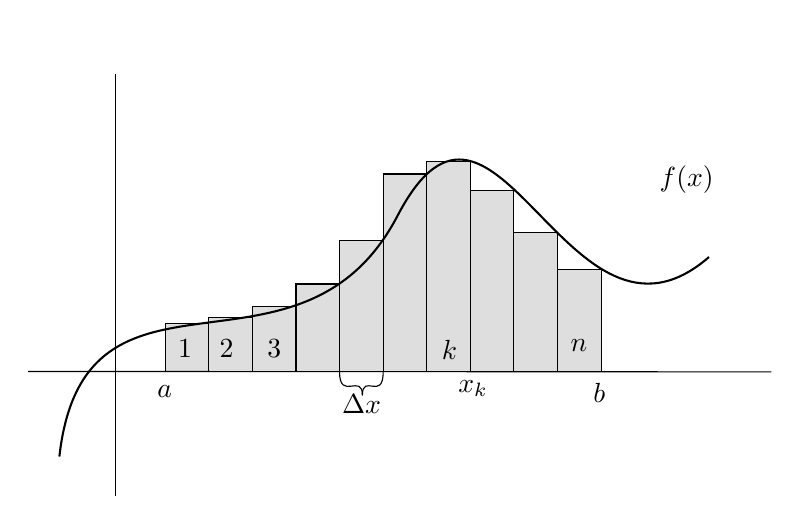
\begin{tikzpicture}[x=0.75pt,y=0.75pt,yscale=-1,xscale=1]
%uncomment if require: \path (0,300); %set diagram left start at 0, and has height of 300

%Shape: Rectangle [id:dp7232780056512873] 
\draw  [fill={rgb, 255:red, 222; green, 222; blue, 222 }  ,fill opacity=1 ] (217,145.67) -- (238,145.67) -- (238,169) -- (217,169) -- cycle ;
%Shape: Rectangle [id:dp9564785112393279] 
\draw  [fill={rgb, 255:red, 222; green, 222; blue, 222 }  ,fill opacity=1 ] (238,142.67) -- (259,142.67) -- (259,169) -- (238,169) -- cycle ;
%Shape: Rectangle [id:dp3339762801991184] 
\draw  [fill={rgb, 255:red, 222; green, 222; blue, 222 }  ,fill opacity=1 ] (259,137.67) -- (280,137.67) -- (280,169) -- (259,169) -- cycle ;
%Shape: Rectangle [id:dp8735502353012137] 
\draw  [fill={rgb, 255:red, 222; green, 222; blue, 222 }  ,fill opacity=1 ] (280,126.67) -- (301,126.67) -- (301,169) -- (280,169) -- cycle ;
%Shape: Rectangle [id:dp9736947359557422] 
\draw  [fill={rgb, 255:red, 222; green, 222; blue, 222 }  ,fill opacity=1 ] (301,105.67) -- (322,105.67) -- (322,169) -- (301,169) -- cycle ;
%Shape: Rectangle [id:dp462370433249887] 
\draw  [fill={rgb, 255:red, 222; green, 222; blue, 222 }  ,fill opacity=1 ] (322,73.67) -- (343,73.67) -- (343,169) -- (322,169) -- cycle ;
%Shape: Rectangle [id:dp30050179546388955] 
\draw  [fill={rgb, 255:red, 222; green, 222; blue, 222 }  ,fill opacity=1 ] (343,67.67) -- (364,67.67) -- (364,169) -- (343,169) -- cycle ;
%Shape: Rectangle [id:dp5888931362167766] 
\draw  [fill={rgb, 255:red, 222; green, 222; blue, 222 }  ,fill opacity=1 ] (364,81.67) -- (385,81.67) -- (385,169) -- (364,169) -- cycle ;
%Shape: Rectangle [id:dp23162244325779224] 
\draw  [fill={rgb, 255:red, 222; green, 222; blue, 222 }  ,fill opacity=1 ] (385,101.67) -- (406,101.67) -- (406,169) -- (385,169) -- cycle ;
%Shape: Rectangle [id:dp5505196011593232] 
\draw  [fill={rgb, 255:red, 222; green, 222; blue, 222 }  ,fill opacity=1 ] (406,119.67) -- (427,119.67) -- (427,169) -- (406,169) -- cycle ;
%Straight Lines [id:da015408719112721014] 
\draw    (151,168.8) -- (509,169) ;
%Straight Lines [id:da7870970100056962] 
\draw    (193,25.67) -- (193,229) ;
%Curve Lines [id:da23517536685350726] 
\draw [line width=0.75]    (166,209.8) .. controls (178,103.67) and (282,183.67) .. (329,93.67) .. controls (376,3.67) and (411,172.67) .. (479,113.67) ;
%Curve Lines [id:da8766831258062089] 
\draw    (301,169) .. controls (301,183.33) and (312,169.33) .. (312,180.33) ;
%Curve Lines [id:da8471782229516964] 
\draw    (322,169) .. controls (322,183.33) and (312,169.33) .. (312,180.33) ;

% Text Node
\draw (212,174.4) node [anchor=north west][inner sep=0.75pt]    {$a$};
% Text Node
\draw (422,173.4) node [anchor=north west][inner sep=0.75pt]    {$b$};
% Text Node
\draw (454,68.4) node [anchor=north west][inner sep=0.75pt]    {$f( x)$};
% Text Node
\draw (222,152.4) node [anchor=north west][inner sep=0.75pt]    {$1$};
% Text Node
\draw (242,152.4) node [anchor=north west][inner sep=0.75pt]    {$2$};
% Text Node
\draw (265,152.4) node [anchor=north west][inner sep=0.75pt]    {$3$};
% Text Node
\draw (411,152.4) node [anchor=north west][inner sep=0.75pt]    {$n$};
% Text Node
\draw (349,152.4) node [anchor=north west][inner sep=0.75pt]    {$k$};
% Text Node
\draw (301,178.73) node [anchor=north west][inner sep=0.75pt]    {$\Delta x$};
% Text Node
\draw (357,171.73) node [anchor=north west][inner sep=0.75pt]    {$x_{k}$};


\end{tikzpicture}

}
\caption{A Right Reimann Sum}
\end{figure}

Divide the interval $(a,b)$ into $n$ equal sub-intervals, each with width $\Delta x= \frac{b-a}{n}$. Then for each sub-interval draw a rectangle with base length $\Delta x$ on the $x$-axis and height determined by the value of $f$ at the right endpoint of the sub-interval. The right endpoint of the $k$th sub-interval is $x_k=a+k\Delta x$, so the area of the $k$th rectangle is $f(x_k) \Delta x$. The area of all $n$ rectangles together is
$$\sum_{k=1}^{n}f(x_k)\Delta x.$$
Since we used the \textit{right} endpoint of each sub-interval, we call this quantity the \textbf{$n$th Right Riemann Sum}:
$$R_n=\sum_{k=1}^{n}f\left(a+k\frac{b-a}{n}\right)\frac{b-a}{n}.$$
We could also have used the \textit{left} endpoint of each sub-interval to determine the height of each box, in which case we would get the \textbf{$n$th Left Riemann Sum}:\mar{Draw a picture of $L_n$.}
$$L_n=\sum_{k=1}^{n}f\left(a+(k-1)\frac{b-a}{n}\right)\frac{b-a}{n}.$$
If instead we use trapezoids above each sub-interval, we get the \textbf{$n$th Trapezoid Riemann Sum}: \mar{Draw a picture of $T_n$.}
$$T_n=\sum_{i=k}^{n}\frac{f\left(a+(k-1)\frac{b-a}{n}\right)+f\left(a+k\frac{b-a}{n}\right)}{2}\frac{b-a}{n}=\frac{R_n+L_n}{2},$$
where the $k$th trapezoid has width $\Delta x$ and heights determined by the left and right endpoints of the $k$th sub-interval. (Remember that a trapezoid with width $w$ and heights $h_1$ and $h_2$ has area $A=\frac{h_1+h_2}{2}w$. \mar{When are $R_n$, $L_n$, and $T_n$ overestimates? Underestimates?}

In practice, it doesn't matter which you choose to compute because of the following theorem:
\begin{thm} With the notation as above,
$$\lim_{n\to\infty}R_n=\lim_{n\to\infty}L_n=\lim_{n\to\infty}T_n=\int_a^bf(x)\ dx.$$
\end{thm}

This theorem should be intuitive: as $n$ gets larger, the width of each rectangle gets smaller and the approximation gets better. More abstractly, this tells us that integration and summation are intimately related: you can think of a definite integral as a sum of infinitely thin boxes with height $f(x)$ and width $dx$, one for ``each'' value of $x$ in $(a,b)$. This perspective will be very helpful later. \mar{Note the similarity in notation between a definite integral and the Riemann sum $$\sum_{k=1}^{n}f(x_k)\Delta x.$$}

For large $n$, a Riemann sum can give a very good approximation, but in general it is not feasible to do by hand. However, if $f$ is a polynomial it is not hard to compute $R_n$ algebraically and then take a limit. In order to do so, we'll need the following summation identities:
\begin{align*}
&\sum_{k=1}^n 1 = n 
& &
\sum_{k=1}^n k = \frac{n(n+1)}{2}\\
&\sum_{k=1}^n k^2 = \frac{n(n+1)(2n+1)}{6}
& &
\sum_{k=1}^n k^3 = \frac{n^2(n+1)^2}{4}
\end{align*}

Here is an example:
\begin{itemize}
    \item To compute $\int_{0}^{1}x^2+x\ dx$, first find $R_n$:
    \begin{align*}
        R_n
        & = \sum_{k=1}^{n}f\left(a+k\frac{b-a}{n}\right)\frac{b-a}{n}\\ 
        & = \sum_{k=1}^n\left(\left(0+k\frac{1-0}{n}\right)^2 + \left(0+k\frac{1-0}{n}\right)\right)\frac{1-0}{n}&&&\text{(plug in)}\\
        & = \sum_{k=1}^n\left(\frac{k^2}{n^2} + \frac{k}{n}\right)\frac{1}{n} &&&\text{(expand and simplify)}\\
        & = \frac{1}{n^3}\sum_{k=1}^nk^2+\frac{1}{n^2}\sum_{k=1}^nk &&& \text{(factor)}\\
        & = \frac{1}{n^3}\frac{n(n+1)(2n+1)}{6}+\frac{1}{n^2}\frac{n(n+1)}{2} &&&\text{(use sum identities)}
    \end{align*}
    Then take the limit:
    $$\lim_{n\to\infty}R_n=\lim_{n\to\infty} \frac{1}{n^3}\frac{n(n+1)(2n+1)}{6}+\frac{1}{n^2}\frac{n(n+1)}{2} = \frac{2}{6} + \frac{1}{2} = \frac{5}{6}.$$
    
\end{itemize}

\mar{Compute $$\int_{0}^1x^3\ dx$$ using the method of Riemann Sums.}

\subsection{The Fundamental Theorem of Calculus}

Let's cut right to the chase:

\begin{thm}[The Fundamental Theorem of Calculus]
    $$\int_a^bf(x)\ dx = F(b)-F(a),$$
    where $F'=f$.
\end{thm}

This theorem is the connection between differentiation and integration! It is also how we will compute definite integrals from now on:
\begin{enumerate}
    \item Find a function $F$ for which $F'=f$.
    \item Evaluate $F(b)-F(a).$
\end{enumerate}

The first point is called \textbf{anti-differentiation}, and is the harder step. Before we get to that, let's try to understand how this theorem agrees with our intuition about Riemann Sums. If we take the $b$-derivative of the equation in the theorem, we get
$$\frac{d}{db}\left[\int_a^{b}f(x)\ dx\right] = \frac{d}{db}\left[F(b)-F(a)\right] = f(b).$$
This means that the rate at which the area is changing is $f(b)$. This makes sense in terms of Riemann sums: if we increase $b$ by a small amount $\Delta b$, the area will change by about $f(b) \Delta b$. Thus the derivative of the area is $f(b)\Delta b/\Delta b = f(b)$. \mar{Draw a picture of $b$ increasing by $\Delta b$. Then sit and really think about this until it makes sense.}














\newpage
\section{The Indefinite Integral}

Since the Fundamental Theorem of Calculus tells us that we have to understand anti-derivatives in order to compute definite integrals, this chapter will focus on this task.


\subsection{Anti-differentiation}


If $F'=f$, we call $F$ an \textbf{anti-derivative} (or \textbf{indefinite integral}) of $f$ and write
$$F(x)=\int f(x)\ dx \quad\text{or}\quad F=\int f.$$ 
Unfortunately, such a function $F$ does not always exist. \mar{Check out this \href{https://xkcd.com/2117}{XKCD Comic}.}



The first thing to understand is that unlike derivatives, anti-derivatives are not unique! This is because constant terms are always killed by differentiation. For example, the derivative of $x^2$ and $x^2+1$ are both $2x$, so both are worthy anti-derivatives for $2x$. To solve this problem, we consider \textit{the} anti-derivative of $f$ to be the collection of \textit{all} functions whose derivative is $f$. These functions only differ by a constant so we write ``$+C$'' at the end of \textit{an} anti-derivative to denote \textit{the} anti-derivative. For example, $\int 2x\ dx = x^2+C$.

Similarly to differentiation, we will build up a two-part collection of tools to tackle integration problems.

\begin{enumerate}
\item rules to break functions up and reassemble

\begin{center}
\def\arraystretch{1.5}
\begin{tabular}{@{}ll@{}}
\toprule[0.4mm]
\textbf{Scalar Multiplication} & $\int a f = a \int f$. \\
\textbf{Sum} & $\int f + \int g= \int f + \int g$ \\
\textbf{Integration by Parts} & $\int f'g = fg - \int fg' $ \\
\textbf{$u$-substitution} & $\int f'(g(x))g'(x)\ dx =  f(g(x))$ \\
% \textbf{$u$-substitution} & $\int (f'\circ g)g' =  f\circ g$ \\
\bottomrule[0.4mm]
\end{tabular}
\end{center}

\item anti-derivatives of ``basic'' functions:

\end{enumerate}


\begin{center}
\def\arraystretch{1.5}
\begin{tabular}{@{}ll@{}}
\toprule[0.4mm]
\textbf{Power Rule}
 & $\int x^a \ dx = \begin{cases}
\frac{1}{a+1}x^{a+1} + C & a \neq -1\\
\ln|x| + C & a = -1
\end{cases}$ \\
\textbf{Trig Rules}  & $\int \sin(x)\ dx = -\cos(x)+C$\\
                     & $\int \cos(x)\ dx = \sin(x)+C$ \\
\textbf{Exponential Rules} & $\int a^x\ dx = \frac{1}{\ln(a)}a^x+C$ \\
\bottomrule[0.4mm]
\end{tabular}
\end{center}

Each of the integration rules are true because of a corresponding rule for derivatives. \mar{Which differentiation rules do Integration by Parts and $u$-substitution correspond to?}

% Here are some examples using these rules:
% \begin{itemize}
%     \item $\int \sin(2x)\ dx = \frac{1}{2} \int 2\sin(2x)\ dx = -\frac{1}{2}\cos(2x) + C$ by $u$-substitution. The ``inside'' function is $2x$, and while its derivative (2) doesn't appear in the integral, we can multiply by $2$ and $\frac{1}{2}$.
% \end{itemize}


\subsection{Partial Fraction Decomposition}

When attempting to integrate a rational function, partial fraction decomposition is a common trick that comes in handy. It effectively breaks a rational function into a sum of rational functions with lower degree denominators.



\begin{center}
\def\arraystretch{1.5}
\begin{tabular}{@{}ll@{}}
\toprule[0.4mm]
      Factor in denominator & Term in decomposition\\
      \hline
      $ax+b$          & $\frac{A}{ax+b}$ \\
      $(ax+b)^k$      & $\frac{A_1}{ax+b}+\frac{A_2}{(ax+b)^2}+\dots+\frac{A_k}{(ax+b)^k}$ \\
      $ax^2+bx+c$     & $\frac{Ax+B}{ax^2+bx+c}$\\
      $(ax^2+bx+c)^k$ & $\frac{A_1x+B_1}{ax^2+bx+c}+\frac{A_2x+B_2}{(ax^2+bx+c)^2}+\dots+\frac{A_kx+B_k}{(ax^2+bx+c)^k}$ \\
\bottomrule[0.4mm]
    \end{tabular}
\end{center}


While this table is not exhaustive, it covers the range of complexity required in a calculus class.

\begin{strat}[Partial Fraction Decomposition]
    
\begin{enumerate}
  \item Factor the denominator of the original rational expression.
  \item Set the original expression equal to the sum of appropriate terms (see table).
  \item Write the sum as a single rational expression by finding a common denominator.
  \item Use the two numerators to solve a system of equations for the unknown values, $A$, $B$, $C$, etc.
\end{enumerate}
\end{strat}



\subsection{Trigonometric Substitution}

Another trick that is useful when integrating is the 




\newpage
\section{More Definite Integrals}

\subsection{Improper Integrals}

\textbf{Improper integrals} are integrals involving infinity. There are two types:
\begin{enumerate}
    \item $\pm\infty$ is in a bound of the integral, or
    \item the function being integrated has a vertical asymptote on the interval of integration.
\end{enumerate}


To evaluate an improper integral, rewrite the integral as a limit of a proper integral, compute the integral as normal, and then take the limit. When evaluating integrals of the second type, make sure you use a sided limit from the inside of the bound of integration.

If the value of the improper integral is a finite quantity, we say the integral \textbf{converges}. If the value is an infinite quantity or the limit DNE, then we say the integral is \textbf{divergent}. Sometimes you might be asked the nature of the divergence (i.e. is the limit equal to $\pm\infty$ or non-existent).

Here's an example of each type:

\begin{itemize}%[leftmargin=1em]
    \item $\displaystyle \int_1^\infty \frac{1}{x^2}\ dx
     = \lim_{a\to \infty}\int_1^a \frac{1}{x^2}\ dx 
     = \lim_{a\to \infty}\left[\frac{-1}{x}\right]_1^a 
     = \lim_{a\to \infty} \left(1-\frac{1}{a}\right)
    =1.$
    \item $\displaystyle\int_{0}^{1}\frac{1}{x^{2}}\ dx 
     = \lim_{a\to 0^+} \int_{a}^{1}\frac{1}{x^{2}}\ dx 
     = \lim_{a\to 0^+}\left[\frac{-1}{x}\right]_a^1 
     = \lim_{a\to 0^+}\left(\frac{1}{a}-1\right)
     = \infty.$
\end{itemize}

\mar{For what values of $p$ does $$\int_0^1 x^p \ dx$$ converge?}

Many times, a vertical asymptote won't be one of the endpoints of the interval. When this happens, split the integral in two, so the VA now lies on the endpoints of the intervals. Here is an example:
\begin{itemize}
	\item $\displaystyle \int_0^3 \frac{1}{x-1} \ dx = \int_0^1 \frac{1}{x-1} \ dx + \int_1^3 \frac{1}{x-1} \ dx$.
\end{itemize}


When the convergence of an integral is all you care about, the following theorem can be helpful.

\begin{theorem}
If $0\leq f(x) \leq g(x)$, then $\int_a^b f(x)\ dx \leq \int_a^b g(x)\ dx$.
\end{theorem}

In particular, this means that if $\int_a^b f(x)\ dx$ diverges, then $\int_a^b g(x)\ dx$ diverges, and if $\int_a^b g(x)\ dx$ converges, then $\int_a^b f(x)\ dx$ converges.


To finish the section, here is an algebraic property of integrals that can come in handy:
\begin{theorem} The following are always true if each integral exists and is finite.
\begin{enumerate}
\item $\displaystyle\int_a^bf(x)\ dx + \int_b^cf(x)\ dx = \int_a^c f(x)\ dx$.
\item $\displaystyle\int_a^bf(x)\ dx = -\int_b^a f(x)\ dx$.
\end{enumerate}
\end{theorem}

\mar{Use 1 to prove 2.}

\subsection{Even and Odd Functions}

A function $f$ is called \textbf{even} if $f(-x)=f(x)$, and is called \textbf{odd} if $f(-x)=-f(x)$. Even functions are symmetric about the $y$-axis, and odd functions are rotationally symmetric around the origin. Therefore, if $f$ is odd,
$$\int_{-a}^af(x)\ dx = 0$$
since the areas bounded by $f$ to the left and right of $x=0$ differ only in sign. Similarly, if $f$ is even,
$$\int_{-a}^af(x)\ dx = 2\int_{0}^af(x)\ dx$$
since the areas bounded by $f$ to the left and right of $x=0$ are the same.
Here are some examples:
\begin{itemize}
\item $\int_{-1}^1\sin(x)\ dx = 0$ since $\sin(-x)=-\sin(x)$.
\item $\int_{-1}^1\cos(x)\ dx = 2\int_0^1\cos(x)\ dx$ since $\cos(-x)=\cos(x)$.
\end{itemize}





\newpage
\section{Applications of Integrals}

Many applications of integrals use the following heuristic idea: you have a value $A$ that you want to compute; you break the problem up into infinitesimal pieces and compute the corresponding infinitesimal value ''$dA$''; then sum up the small values by integrating
$$A=\int\ dA.$$

Understanding integrals as sums will make understanding these integral applications easier.
The first example of this you will see is computing areas. \mar{Try to find all such examples.}

\subsection{Average Values}

The average value of $f$ on $[a,b]$ is 
$$\frac{\displaystyle\int_a^bf(x)\ dx}{b-a}.$$
There are various intuitive explanations of this; here are two.

\subsubsection{Water in a tank}
Imagine water is sloshing around in a tank and the height of the water at a particular time is described by a function $f(x)$ (see the figure below). 

\begin{figure}[H]
\centering

\phantom{}
\vspace{1em}



\tikzset{every picture/.style={line width=0.75pt}} %set default line width to 0.75pt        

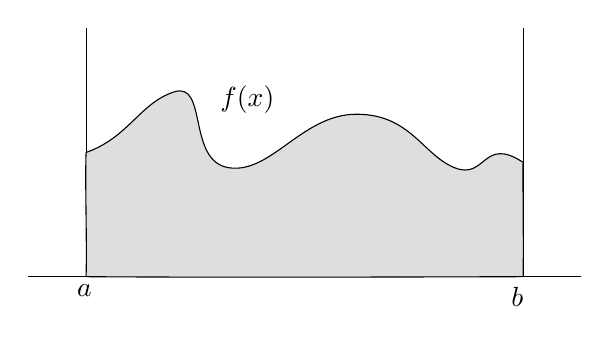
\begin{tikzpicture}[x=0.75pt,y=0.75pt,yscale=-1,xscale=1]
%uncomment if require: \path (0,409); %set diagram left start at 0, and has height of 409

%Straight Lines [id:da044590240587294216] 
\draw    (109.67,150.03) -- (376,150.03) ;
%Straight Lines [id:da5673860317913473] 
\draw    (137.55,30.33) -- (137.55,150.03) ;
%Shape: Polygon Curved [id:ds7088187846595497] 
\draw  [fill={rgb, 255:red, 222; green, 222; blue, 222 }  ,fill opacity=1 ] (179.85,61.03) .. controls (196.34,55.58) and (185.98,94.48) .. (206.35,97.55) .. controls (226.71,100.62) and (241.59,71.86) .. (267.7,71.77) .. controls (293.81,71.67) and (299.9,91.52) .. (315.11,97.55) .. controls (330.32,103.59) and (328.57,82.06) .. (348.09,94.95) .. controls (347.87,101.17) and (348.41,132.15) .. (348.11,150.03) .. controls (249.57,150.34) and (179.85,150.34) .. (137.55,150.03) .. controls (138,133) and (137,104) .. (137.55,90.18) .. controls (158,83) and (163.37,66.47) .. (179.85,61.03) -- cycle ;
%Straight Lines [id:da25646989795162733] 
\draw [color={rgb, 255:red, 0; green, 0; blue, 0 }  ,draw opacity=1 ]   (348.11,30.33) -- (348.11,150.03) ;

% Text Node
\draw (132.02,152.57) node [anchor=north west][inner sep=0.75pt]    {$a$};
% Text Node
\draw (341.18,154.1) node [anchor=north west][inner sep=0.75pt]    {$b$};
% Text Node
\draw (201.02,56.84) node [anchor=north west][inner sep=0.75pt]    {$f( x)$};


\end{tikzpicture}
\vspace{1em}

\phantom{}

\end{figure}

The average value of $f(x)$ on $[a,b]$ is the height of the water once it settles. To find this height, find the area of the water $\left(\displaystyle\int_a^bf(x)\ dx\right)$ and divide by the width of the tank ($b-a$).

\subsubsection{Using the FTC and Average Slope}
Let $F$ be an antiderivative of $f$. Then the average value of $f(x)$ on $[a,b]$ is equal to the average value of $F'$ on $[a,b]$. We know how to calculate this using the slope of a secant line:
$$\frac{F(b)-F(a)}{b-a}\overset{FTC}{=}\frac{\int_a^bf(x) \ dx}{b-a}.$$


% \subsection{Reimann Sums}
% The average of $f$ on a finite set $A=\{x_1,\dots, x_n\}$ is the sum of $f(x)$ evaluated at every element of $A$, divided by the number of elements of $A$:
% $$\frac{\sum_{i=1}^nf(x_i)}{n}.$$
\mar{Use Reimann sums to get another explanation.}


\subsection{Areas}
To compute the area $A$ between $f(x)$ and $g(x)$ on $[a,b]$, imagine dividing up the area into infinitesimally small strips, each with height $f(x)-g(x)$ and (infinitesimal) width $dx$. The area of the strip is therefore $dA=(f(x)-g(x))\ dx$. One such strip is shown on the graph below (the width enlarged to be visible). To compute the desired area, simply integrate $dA$ over $[a,b]$:
$$A=\int dA = \int_a^b(f(x)-g(x))\ dx.$$

\begin{figure}[H]
\centering

\tikzset{every picture/.style={line width=0.75pt}} %set default line width to 0.75pt        

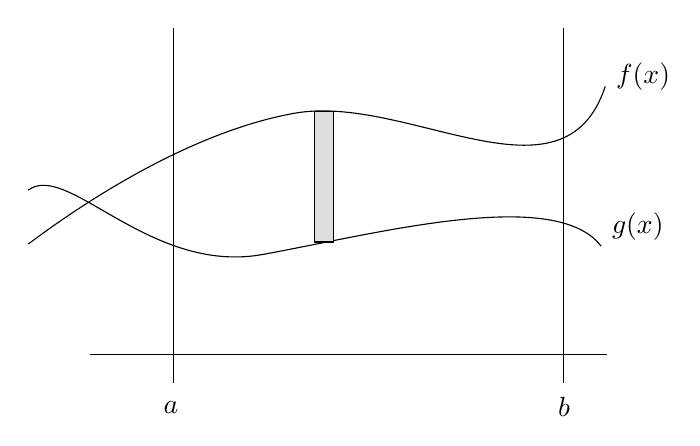
\begin{tikzpicture}[x=0.75pt,y=0.75pt,yscale=-1,xscale=1]
%uncomment if require: \path (0,300); %set diagram left start at 0, and has height of 300

%Straight Lines [id:da5705104580473277] 
\draw    (182,27) -- (182,198) ;
%Straight Lines [id:da838729158622765] 
\draw    (370,27) -- (370,198) ;
%Straight Lines [id:da13279837061190713] 
\draw    (391,184) -- (142,184) ;
%Curve Lines [id:da08034929661214907] 
\draw    (112,131) .. controls (130.83,116.88) and (185.53,77.9) .. (240,68) .. controls (294.47,58.1) and (370,116) .. (390,55) ;
%Curve Lines [id:da13490737944947462] 
\draw    (112,105) .. controls (130.83,90.88) and (170.53,145.9) .. (225,136) .. controls (279.47,126.1) and (366,103) .. (388,132) ;
%Shape: Rectangle [id:dp8230016382923657] 
\draw  [fill={rgb, 255:red, 222; green, 222; blue, 222 }  ,fill opacity=1 ] (250,67) -- (259,67) -- (259,130) -- (250,130) -- cycle ;

% Text Node
\draw (394,42.4) node [anchor=north west][inner sep=0.75pt]    {$f( x)$};
% Text Node
\draw (392,114.4) node [anchor=north west][inner sep=0.75pt]    {$g( x)$};
% Text Node
\draw (176,205.4) node [anchor=north west][inner sep=0.75pt]    {$a$};
% Text Node
\draw (366,203.4) node [anchor=north west][inner sep=0.75pt]    {$b$};

\end{tikzpicture}

\end{figure}



\subsection{Arc Length}

The \textbf{arc length} of $f(x)$ on $[a,b]$ is the length of string needed to trace the graph of $f$ on the interval $[a,b]$. Similarly to computing areas, to compute the arc length $L$ of a function $f$'s graph, divide the length into infinitesimally short segments (that we assume to be linear). Then each segment's length can be computed using the pythagorean theorem (see picture below): 
$$dL=\sqrt{dx^2+dy^2}=\sqrt{1+\frac{dy^2}{dx^2}}\ dx=\sqrt{1+f'(x)^2}\ dx.$$
Then to compute the arc length $L$, sum $dL$ over $[a,b]$ by integrating:
$$L=\int_a^b\sqrt{1+f'(x)^2}\ dx.$$

\begin{figure}[H]
\centering

\tikzset{every picture/.style={line width=0.75pt}} %set default line width to 0.75pt        

\begin{tikzpicture}[x=0.75pt,y=0.75pt,yscale=-1,xscale=1]
%uncomment if require: \path (0,300); %set diagram left start at 0, and has height of 300

%Straight Lines [id:da8511908828152182] 
\draw    (202,47) -- (202,218) ;
%Straight Lines [id:da8667346744151081] 
\draw    (390,47) -- (390,218) ;
%Straight Lines [id:da41300492628810637] 
\draw    (411,204) -- (162,204) ;
%Curve Lines [id:da05101594018896982] 
\draw    (149,184) .. controls (167.83,169.88) and (219.53,162.9) .. (274,153) .. controls (328.47,143.1) and (319,63) .. (410,75) ;
%Shape: Triangle [id:dp7671239003370118] 
\draw  [line width=1.5]  (333,101) -- (333,133) -- (308,133) -- cycle ;

% Text Node
\draw (414,62.4) node [anchor=north west][inner sep=0.75pt]    {$f( x)$};
% Text Node
\draw (196,225.4) node [anchor=north west][inner sep=0.75pt]    {$a$};
% Text Node
\draw (386,223.4) node [anchor=north west][inner sep=0.75pt]    {$b$};
% Text Node
\draw (310,136.4) node [anchor=north west][inner sep=0.75pt]    {$dx$};
% Text Node
\draw (337,109.4) node [anchor=north west][inner sep=0.75pt]    {$dy$};
% Text Node
\draw (299,100.4) node [anchor=north west][inner sep=0.75pt]    {$dL$};


\end{tikzpicture}

\end{figure}





\subsection{Probability}

Imagine we have an experiment, and every time it is performed the outcome is a real number. (Think throwing a dart at the plane, and the outcome is the $x$ coordinate of the point it lands on). 

To start, the we will define an \textbf{event} to be a subset of $\R$. Given such a subset $A\subset\R$, our goal is to describe the probability that the outcome $X$ is in $A$. We denote this $\P(X\in A)$.


For the kinds of experiments we will consider, we will assume that it is never possible to get the same outcome twice. This means that the probability of any \textit{particular} outcome is 0: for any $a\in\R$, $$\P(X\in\{a\})=\P(X=a)=0.$$ 
This might seem paradoxical, because the dart must hit \textit{some} point. However, it should make sense since there are infinitely many possible outcomes.
\mar{Think about this carefully.}

To compute $\P(X\in A)$ in general, we need a way to describe an allocation of probability specific to the experiment that is happening. For this (of course) we use a a function! A bounded function $f:\R \to \R$ is called a \textbf{probability density function} (PDF) if it is non-negative and $\int_{\infty}^\infty f(x)\ dx= 1$.\mar{What does the condition $$\int_{\infty}^\infty f(x)\ dx= 1$$ mean in terms of probability?} 
To compute a probability, we just have to integrate:
$$\P(X\in A) = \int_A f(x)\ dx.$$
This notation means that if $A$ is the union of disjoint intervals, integrate over each interval and add the results. In particular, if $A=(a,b)$, then 
$$\P(X\in A) = \int_a^b f(x)\ dx.$$
The anti-derivative function
$$F(x)=\P(X<x) = \int_{-\infty}^x f(t)\ dt$$
is called the \textbf{cumulative distribution function} (CDF). Here are some examples:
\begin{itemize}
\item The ``uniform'' PDF on $(0,1)$ is defined as
$$f(x)=\begin{cases}0 & x < 0\\ 1 & 0\leq x\leq 1\\ 0 & x>1\end{cases}
\quad\quad\text{ and } \quad\quad
F(x)=\begin{cases}0 & x < 0\\ x & 0\leq x\leq 1\\ 1 & x>1\end{cases}$$
is its CDF. The probability that an outcome of an experiment governed by this PDF is greater than $1/4$ is
$$\P\left(X\in(1/4,\infty)\right)
= \int_{\frac14}^{\infty}f(x)\ dx
= \int_{\frac14}^{1}1\ dx + \int_{1}^{\infty}0\ dx 
= \frac34.
$$
The probability that an outcome is in $(0,1/2)\cup(2/3,1)$ is
$$\P\left(X\in(0,1/2)\cup(2/3,1)\right)
= \int_0^{\frac12}1\ dx + \int_{\frac23}^11\ dx
= \frac12+\frac13 = \frac56.
$$

\item  The ``exponential'' PDF is defined as
$$f(x)=\begin{cases}0 & x < 0\\ e^{-x} & x\geq 0\end{cases}
\quad\quad\text{ and } \quad\quad
F(x)=\begin{cases}0 & x < 0\\1- e^{-x} & x\geq 0\end{cases}$$
is its CDF. This PDF is often used to model the wait time between phone calls. The probability that an outcome of an experiment governed by this PDF is greater than $1/4$ is
$$\P\left(X\in(1/4,\infty)\right)
= \int_{\frac14}^{\infty} e^{-x}\ dx
= e^{-\frac{1}{4}}.
$$

\end{itemize}


\mar{Draw a picture of these PDFs and CDFs.}



\subsection{Volumes and Surface Area}


\subsection{Moments and Centroids}


\subsection{Work}


\newpage
\part{Sequences and Series}
\section{Sequences}

A \textbf{sequence} of real numbers is an ordered and infinite list of real numbers.



\section{Tests for Convergence and Divergence}



Let $(a_n)$ be a sequence, and define a new sequence $(s_n)$ of ``partial sums'' by
$$s_n=\sum_{i=1}^n a_i = a_1 + \cdots + a_n.$$
We write 
$$\lim _{n \to \infty} s_{n}=\lim _{n \to \infty} \sum_{i=1}^{n} a_{i}=\sum_{i=1}^{\infty} a_{i}=\sum a_n$$
and call $\sum a_n$ an \textbf{infinite series}. We are interested in when this quantity is finite:
\begin{itemize}
    \item If $\lim _{n \to \infty} s_{n}$ is finite, we say that $\sum a_n$ is \textbf{convergent} (or that $\sum a_n$ converges).
    \item  When $\lim _{n \to \infty} s_{n}$ is infinite, we say that $\sum a_n$ is \textbf{divergent} (or that $\sum a_n$ diverges).
\end{itemize}

\vspace{.5em}

\begin{thm}[Divergence Test] If $\displaystyle \lim_{n\to\infty}a_n\neq 0$, then $\sum a_n$ will diverge.
\end{thm}


\begin{thm}[Integral Test]
Suppose that $f(x)$ is a continuous, positive, and decreasing function on the interval $[k,\infty)$ and that $f(n)=a_n$. Then
$$\int_k^\infty f(x)\ dx\text{ is convergent} \iff \sum_{n=k}^\infty a_n\text{ is convergent}.$$
\end{thm}


\begin{thm}[The $p$-series Test]
If $k>0$, then $\sum_{n=k}^\infty\frac{1}{n^p}$ converges if $p>1$ and diverges if $p\leq 1$.
\end{thm}




\begin{thm}[Comparison Test]
Suppose that we have two series $\sum a_n$ and $\sum b_n$, with $0\leq a_n\leq b_n$ for all $n$. Then
$$\sum b_n\text{ converges}\implies \sum a_n\text{ converges}$$
and (by contraposition)
$$\sum a_n\text{ diverges}\implies \sum b_n\text{ diverges}.$$
\end{thm}




\begin{thm}[Limit Comparison Test]
Suppose that we have two series $\sum a_n$ and $\sum b_n$ with $a_n\geq 0$ and $b_n > 0$ for all $n$. Define
$$c=\lim_{n\to\infty}\frac{a_n}{b_n}.$$
If $c$ is positive and finite, then either both series converge of both series diverge.
\end{thm}



\begin{thm}[Alternating Series Test]
Suppose that we have a series $\sum a_{n}$ and either $$a_{n}=(-1)^{n} b_{n}\quad\text{ or }\quad  a_{n}=(-1)^{n+1} b_{n}$$ where $b_{n} \geq 0$ for all $n .$ Then if,
\begin{enumerate}
    \item $\displaystyle\lim _{n \to \infty} b_{n}=0$ and
    \item $\left\{b_{n}\right\}$ is a decreasing sequence
\end{enumerate}
the series $\sum a_{n}$ is convergent.
\end{thm}


\begin{thm}[Absolute Convergence Test]
\phantom{}
\begin{itemize}[leftmargin=1em]
    \item If the series $\sum |a_n|$ is convergent, then $\sum a_n$ is called \textbf{absolutely convergent}, and must also be convergent.
    \item If $\sum a_n$ converges but $\sum |a_n|$ diverges, then the series $\sum a_n$ is called \textbf{conditionally convergent}.
\end{itemize}
\end{thm}


\begin{thm}[Ratio Test]
Suppose we have the series $\sum a_{n}$. Define,
$$L=\lim _{n \to \infty} \left|\frac{a_{n+1}}{a_{n}}\right|.$$
Then,
\begin{enumerate}[leftmargin=1em]
    \item if $L<1$ the series is absolutely convergent (and hence convergent).
    \item if $L>1$ the series is divergent.
    \item  if $L=1$ the series may be divergent, conditionally convergent, or absolutely convergent.
\end{enumerate}
\end{thm}

\begin{thm}[Root Test]
Suppose that we have the series $\sum a_{n}$. Define,
$$L=\lim _{n \to \infty} \sqrt[n]{\left|a_{n}\right|}=\lim _{n \rightarrow \infty}\left|a_{n}\right|^{\frac{1}{n}}.$$
Then,
\begin{enumerate}[leftmargin=1em]
    \item if $L<1$ the series is absolutely convergent (and hence convergent).
    \item if $L>1$ the series is divergent.
    \item if $L=1$ the series may be divergent, conditionally convergent, or absolutely convergent.
\end{enumerate}
\end{thm}

\newpage
\section{Power Series}


% \newpage
% \part{Exercises}
% Limits are important in calculus since we need very small quantities to effectively study change. Yeah, that's pretty vague, but hopefully it'll clear up in a few pages.

We study limits for many reasons. One of them is to study functions at points where they are only ``close'' to being defined. Another is to make quantities very (arbitrarily) small, without making them 0.

Here is an example of a practical use of limits. The following two functions' graphs are exactly the same, except at $x=1$.

\begin{figure}[h!]
    \centering
    \fbox{
    \resizebox{4in}{!}{


\tikzset{every picture/.style={line width=0.75pt}} %set default line width to 0.75pt        

\begin{tikzpicture}[x=0.75pt,y=0.75pt,yscale=-1,xscale=1]
%uncomment if require: \path (0,300); %set diagram left start at 0, and has height of 300

%Straight Lines [id:da5436445771795901] 
\draw  [dash pattern={on 0.84pt off 2.51pt}]  (392,151.33) -- (318,151.17) ;
%Straight Lines [id:da6949730842855149] 
\draw  [dash pattern={on 0.84pt off 2.51pt}]  (392,151.33) -- (392,219.5) ;
%Straight Lines [id:da8209687086477877] 
\draw    (49,79.83) -- (49,231.5) ;
%Curve Lines [id:da9233668280128751] 
\draw    (41,186.5) .. controls (59,138.83) and (98,184.83) .. (123,152.83) ;
%Curve Lines [id:da7989009557315903] 
\draw    (123,152.83) .. controls (150,110.83) and (183,173.83) .. (223,143.83) ;

%Straight Lines [id:da6182960293771871] 
\draw    (233,221) -- (39,221) ;
%Straight Lines [id:da04200773563301774] 
\draw    (317,79.83) -- (317,231.5) ;
%Straight Lines [id:da726566232707935] 
\draw    (501,220.5) -- (307,220.5) ;
%Curve Lines [id:da20535665951890536] 
\draw    (309,186.5) .. controls (327,138.83) and (366,184.83) .. (391,152.83) ;
%Curve Lines [id:da8509447981009293] 
\draw    (391,152.83) .. controls (418,110.83) and (451,173.83) .. (491,143.83) ;
%Shape: Circle [id:dp8197107597318569] 
\draw  [fill={rgb, 255:red, 255; green, 255; blue, 255 }  ,fill opacity=1 ] (388.5,151.33) .. controls (388.5,149.4) and (390.07,147.83) .. (392,147.83) .. controls (393.93,147.83) and (395.5,149.4) .. (395.5,151.33) .. controls (395.5,153.27) and (393.93,154.83) .. (392,154.83) .. controls (390.07,154.83) and (388.5,153.27) .. (388.5,151.33) -- cycle ;

%Straight Lines [id:da7228354618576209] 
\draw  [dash pattern={on 0.84pt off 2.51pt}]  (123,152.83) -- (123,221) ;
%Straight Lines [id:da24003054824236258] 
\draw  [dash pattern={on 0.84pt off 2.51pt}]  (123,152.83) -- (49,152.67) ;

% Text Node
\draw (119,227.4) node [anchor=north west][inner sep=0.75pt]    {$1$};
% Text Node
\draw (388.5,227.4) node [anchor=north west][inner sep=0.75pt]    {$1$};
% Text Node
\draw (26,145) node [anchor=north west][inner sep=0.75pt]    {$10$};
% Text Node
\draw (294,145) node [anchor=north west][inner sep=0.75pt]    {$10$};


\end{tikzpicture}

    }}
    \caption{Two functions with the same limits}
\end{figure}

The first function is defined at $x=1$, while the second function is not. However, the values of the second function are near 10 when $x$ is near 1. There is still something useful we can say about the second function at 1: ``the \textit{limit} at 1 is 10.''



\section{Definitions}

\subsection{The Limit}

The intuitive idea of a \textbf{limit} is to examine what the output of a function does as the input moves close to a specific value. We say that the limit of $f$ at $a$ is $L$ if $f(x)$ moves closer to $L$ as as $x$ moves closer to $a$. Note that $f$ need not be defined at $a$ to find the limit of $f$ as $x$ approaches $a$ (in fact, that's the whole point!).

Since the functions we care about take real numbers as inputs, there are two ways you can approach a number on the real line (from the left and from the right). We will talk about left- and right-sided limits.

If $f$ is defined on an interval to the \textit{left} of $a$ (with $a$ as an endpoint) and the values of $f(x)$ approach $L$ as $x$ approaches $a$ from the \textit{left}, we say that the ``\textbf{left-sided limit of $f$ as $x$ approaches $a$} is $L$'' and we write $$\lim_{x\to a^-}f(x)=L.$$
If $f$ is defined on an interval to the \textit{right} of $a$ (with $a$ as an endpoint) and the values of $f(x)$ approach $L$ as $x$ approaches $a$ from the \textit{right}, we say that the \textbf{right-sided limit of $f$ as $x$ approaches $a$} is $L$'' and we write
$$\lim_{x\to a^+}f(x)=L.$$
If the right and left sided limits match, then we say that the \textbf{limit of $f$ as $x$ approaches $a$ is $L$} and write $$\lim_{x\to a}f(x)=L.$$

If the left and right sided limits, do not match, then we say that the limit \textbf{does not exist} (DNE).

One can compute $f(x)$ for values of $x$ that get closer and closer to either side of $a$. If the values approach $L$, then you have good reason to believe that $L$ is the (right- and/or left-sided) limit.

\begin{center}
\begin{tabular}{@{}ll@{}}
\toprule[0.4mm]
   $x$        & $f(x)$        \\
\midrule
   $a-0.1$    & $f(a-0.1)$    \\
   $a-0.01$   & $f(a-0.01)$   \\
   $a-0.001$  & $f(a-0.001)$  \\
   $a-0.0001$ & $f(a-0.0001)$ \\
\midrule
   $a+0.0001$ & $f(a+0.0001)$ \\
   $a+0.001$  & $f(a+0.001)$  \\
   $a+0.01$   & $f(a+0.01)$   \\
   $a+0.1$    & $f(a+0.1)$    \\
\bottomrule[0.4mm]
\end{tabular}
\end{center}
Such calculations, however, cannot prove that a function limits to a specific value.


\subsection{Infinite Limits}

We can extend the idea of limits outside of the real numbers to include positive and negative infinity in place of both $a$ and $L$.
\begin{itemize}
\item If $f(x)$ grows without bound as $x$ approaches $a$ from the left, then we write $$\lim_{x\to a^-}f(x)=\infty.$$
(Similarly for $x$ approaching $a$ from the right, and also if $f(x)$ becomes increasingly negative without bound).
\item We denote the value (if such a value exists) that $f(x)$ approaches as $x$ approaches $\infty$ as $$\lim_{x\to\infty} f(x).$$
(Similarly if $x$ approaches $-\infty$).
\end{itemize}


\subsection{Optional: The $\varepsilon-\delta$ Definition}

You may be dissatisfied with the intuitive approach to limits, so we can make the definition more rigorous. The main idea that needs to be captured by a formal definition is \textit{arbitrary precision}. That is, we need a way to say formally that ``$f(x)$ approaches $L$ as $x$ approaches $a$.''

By controlling the input $x$, we must be able to make the distance $|f(x)-L|$ between the output $f(x)$ and $L$ to be as small as we want (``arbitrarily small''). In other words, if $\varepsilon>0$ is any small positive number, we must be able to ensure (by controlling $x$) that $|f(x)-L| < \varepsilon$. To control $x$, we can make the distance $|x-a|$ between $x$ and $a$ smaller than some positive number $\delta > 0$ (that may depend on $\varepsilon$).

Now we're ready for the real ``$\varepsilon-\delta$'' definition of a limit: we say that \textbf{$L$ is the limit of $f$ as $x$ approaches $a$} if
$$\text{for all } \varepsilon > 0, \text{ there is some } \delta > 0, \text{ such that } |x - a| < \delta \implies |f(x) - L| <\varepsilon.$$

\mar{Read that definition a few times, because statements with multiple quantifiers can be tricky!}

\begin{figure}[h!]
\centering
\fbox{
\tikzset{every picture/.style={line width=0.75pt}}
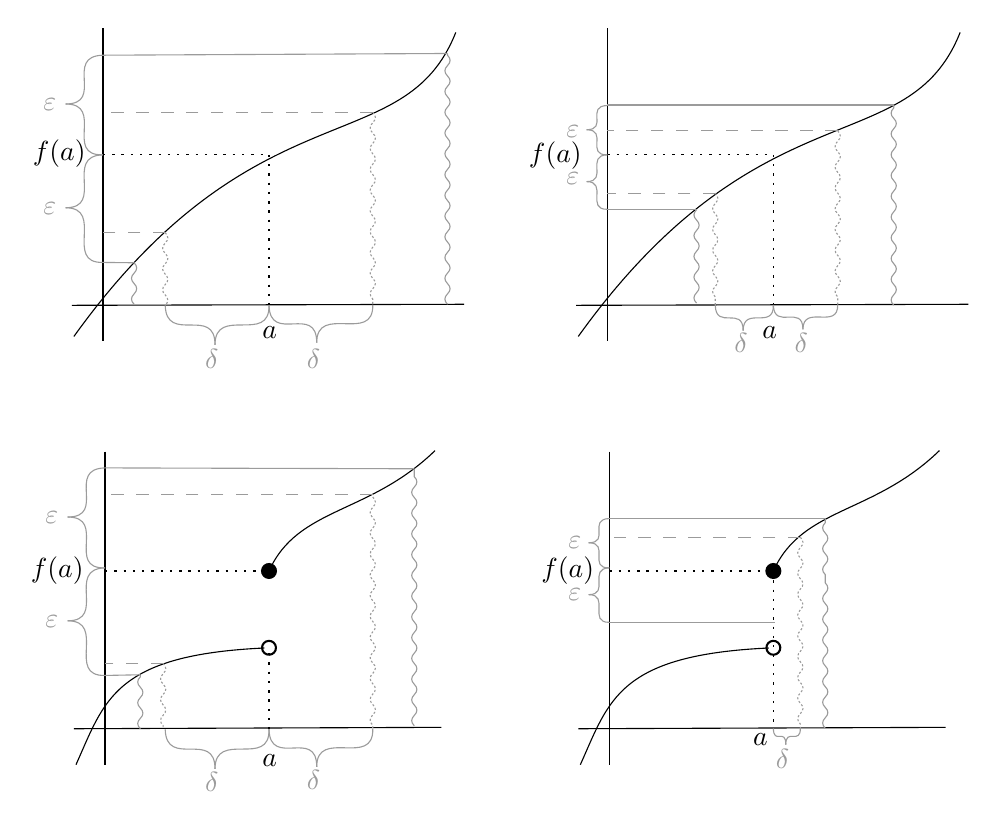
\begin{tikzpicture}[x=0.75pt,y=0.75pt,yscale=-1,xscale=1]
%uncomment if require: \path (0,428); %set diagram left start at 0, and has height of 428

%Straight Lines [id:da2730924968926851]
\draw    (71,155) -- (260,154.5) ;
%Straight Lines [id:da38663844155403493]
\draw    (86,21.5) -- (86,172.33) ;
%Curve Lines [id:da5832897062677318]
\draw    (72,170) .. controls (160,47.5) and (231,86.5) .. (256,23.5) ;
%Curve Lines [id:da15926967534570857]
\draw    (73,376.33) .. controls (86.86,345.64) and (90.92,323.45) .. (163.77,320.1) ;
\draw [shift={(166,320)}, rotate = 357.71] [color={rgb, 255:red, 0; green, 0; blue, 0 }  ][line width=0.75]      (0, 0) circle [x radius= 3.35, y radius= 3.35]   ;
%Curve Lines [id:da573129079856388]
\draw    (166,283) .. controls (180,252) and (214,256) .. (246,225) ;
\draw [shift={(166,283)}, rotate = 294.3] [color={rgb, 255:red, 0; green, 0; blue, 0 }  ][fill={rgb, 255:red, 0; green, 0; blue, 0 }  ][line width=0.75]      (0, 0) circle [x radius= 3.35, y radius= 3.35]   ;
%Straight Lines [id:da06544192635535961]
\draw  [dash pattern={on 0.84pt off 2.51pt}]  (166,82.5) -- (166,154.92) ;
%Straight Lines [id:da8462520068785757]
\draw  [dash pattern={on 0.84pt off 2.51pt}]  (86,82.5) -- (166,82.5) ;
%Straight Lines [id:da8033956316212987]
\draw [color={rgb, 255:red, 155; green, 155; blue, 155 }  ,draw opacity=1 ]   (86,34.5) -- (252,33.67) ;
%Straight Lines [id:da9058328806059841]
\draw [color={rgb, 255:red, 155; green, 155; blue, 155 }  ,draw opacity=1 ]   (86,134.33) -- (101,134.5) ;
%Straight Lines [id:da7683874289412185]
\draw    (72,359) -- (249,358.33) ;
%Straight Lines [id:da21021021460529377]
\draw    (87,225.5) -- (87,376.33) ;
%Straight Lines [id:da5263630709862186]
\draw  [dash pattern={on 0.84pt off 2.51pt}]  (166,322.58) -- (166,359.25) ;
%Straight Lines [id:da2255352189878881]
\draw  [dash pattern={on 0.84pt off 2.51pt}]  (87,283) -- (166,283) ;
%Straight Lines [id:da12241776303117424]
\draw [color={rgb, 255:red, 155; green, 155; blue, 155 }  ,draw opacity=1 ]   (87,233.33) -- (236,233.75) ;
%Straight Lines [id:da6551551228954233]
\draw [color={rgb, 255:red, 155; green, 155; blue, 155 }  ,draw opacity=1 ]   (87,333.33) -- (104,333) ;
%Straight Lines [id:da3470258564776276]
\draw [color={rgb, 255:red, 155; green, 155; blue, 155 }  ,draw opacity=1 ] [dash pattern={on 0.75pt off 0.75pt}]  (116,120) .. controls (117.67,121.67) and (117.67,123.33) .. (116,125) .. controls (114.33,126.67) and (114.33,128.33) .. (116,130) .. controls (117.67,131.67) and (117.67,133.33) .. (116,135) .. controls (114.33,136.67) and (114.33,138.33) .. (116,140) .. controls (117.67,141.67) and (117.67,143.33) .. (116,145) .. controls (114.33,146.67) and (114.33,148.33) .. (116,150) .. controls (117.67,151.67) and (117.67,153.33) .. (116,155) -- (116,155) ;
%Straight Lines [id:da2371091562631653]
\draw [color={rgb, 255:red, 155; green, 155; blue, 155 }  ,draw opacity=1 ] [dash pattern={on 0.75pt off 0.75pt}]  (216,62) .. controls (217.67,63.67) and (217.67,65.33) .. (216,67) .. controls (214.33,68.67) and (214.33,70.33) .. (216,72) .. controls (217.67,73.67) and (217.67,75.33) .. (216,77) .. controls (214.33,78.67) and (214.33,80.33) .. (216,82) .. controls (217.67,83.67) and (217.67,85.33) .. (216,87) .. controls (214.33,88.67) and (214.33,90.33) .. (216,92) .. controls (217.67,93.67) and (217.67,95.33) .. (216,97) .. controls (214.33,98.67) and (214.33,100.33) .. (216,102) .. controls (217.67,103.67) and (217.67,105.33) .. (216,107) .. controls (214.33,108.67) and (214.33,110.33) .. (216,112) .. controls (217.67,113.67) and (217.67,115.33) .. (216,117) .. controls (214.33,118.67) and (214.33,120.33) .. (216,122) .. controls (217.67,123.67) and (217.67,125.33) .. (216,127) .. controls (214.33,128.67) and (214.33,130.33) .. (216,132) .. controls (217.67,133.67) and (217.67,135.33) .. (216,137) .. controls (214.33,138.67) and (214.33,140.33) .. (216,142) .. controls (217.67,143.67) and (217.67,145.33) .. (216,147) .. controls (214.33,148.67) and (214.33,150.33) .. (216,152) -- (216,154.71) -- (216,154.71) ;
%Straight Lines [id:da47940446384008517]
\draw [color={rgb, 255:red, 155; green, 155; blue, 155 }  ,draw opacity=1 ] [dash pattern={on 4.5pt off 4.5pt}]  (116,120) -- (86,120) ;
%Straight Lines [id:da2718218581855085]
\draw [color={rgb, 255:red, 155; green, 155; blue, 155 }  ,draw opacity=1 ] [dash pattern={on 4.5pt off 4.5pt}]  (216,62) -- (86,62) ;
%Curve Lines [id:da7867325499156288]
\draw [color={rgb, 255:red, 155; green, 155; blue, 155 }  ,draw opacity=1 ]   (68,58) .. controls (87,58) and (67,35) .. (86,34.5) ;
%Curve Lines [id:da8389021578247982]
\draw [color={rgb, 255:red, 155; green, 155; blue, 155 }  ,draw opacity=1 ]   (68,58) .. controls (87,58) and (67,83) .. (86,82.5) ;
%Curve Lines [id:da6940267896547274]
\draw [color={rgb, 255:red, 155; green, 155; blue, 155 }  ,draw opacity=1 ]   (68,108) .. controls (87,108) and (67,83) .. (86,82.5) ;
%Curve Lines [id:da9368251006708403]
\draw [color={rgb, 255:red, 155; green, 155; blue, 155 }  ,draw opacity=1 ]   (68,108) .. controls (87,108) and (67,134.83) .. (86,134.33) ;
%Curve Lines [id:da7416463958304471]
\draw [color={rgb, 255:red, 155; green, 155; blue, 155 }  ,draw opacity=1 ]   (139.99,174) .. controls (140,155) and (116.5,174) .. (116,155) ;
%Curve Lines [id:da0946019041451891]
\draw [color={rgb, 255:red, 155; green, 155; blue, 155 }  ,draw opacity=1 ]   (139.99,174) .. controls (140,155) and (166.5,173.92) .. (166,154.92) ;
%Curve Lines [id:da8479225025412045]
\draw [color={rgb, 255:red, 155; green, 155; blue, 155 }  ,draw opacity=1 ]   (188.99,173) .. controls (189,154) and (166.5,173.92) .. (166,154.92) ;
%Curve Lines [id:da5287374586288269]
\draw [color={rgb, 255:red, 155; green, 155; blue, 155 }  ,draw opacity=1 ]   (188.99,173) .. controls (189,154) and (216.5,173.71) .. (216,154.71) ;
%Straight Lines [id:da5763369512697336]
\draw [color={rgb, 255:red, 155; green, 155; blue, 155 }  ,draw opacity=1 ]   (101,154.5) .. controls (99.33,152.83) and (99.33,151.17) .. (101,149.5) .. controls (102.67,147.83) and (102.67,146.17) .. (101,144.5) .. controls (99.33,142.83) and (99.33,141.17) .. (101,139.5) .. controls (102.67,137.83) and (102.67,136.17) .. (101,134.5) -- (101,134.5) ;
%Straight Lines [id:da9925497456851824]
\draw [color={rgb, 255:red, 155; green, 155; blue, 155 }  ,draw opacity=1 ]   (252,154.5) .. controls (250.33,152.83) and (250.33,151.17) .. (252,149.5) .. controls (253.67,147.83) and (253.67,146.17) .. (252,144.5) .. controls (250.33,142.83) and (250.33,141.17) .. (252,139.5) .. controls (253.67,137.83) and (253.67,136.17) .. (252,134.5) .. controls (250.33,132.83) and (250.33,131.17) .. (252,129.5) .. controls (253.67,127.83) and (253.67,126.17) .. (252,124.5) .. controls (250.33,122.83) and (250.33,121.17) .. (252,119.5) .. controls (253.67,117.83) and (253.67,116.17) .. (252,114.5) .. controls (250.33,112.83) and (250.33,111.17) .. (252,109.5) .. controls (253.67,107.83) and (253.67,106.17) .. (252,104.5) .. controls (250.33,102.83) and (250.33,101.17) .. (252,99.5) .. controls (253.67,97.83) and (253.67,96.17) .. (252,94.5) .. controls (250.33,92.83) and (250.33,91.17) .. (252,89.5) .. controls (253.67,87.83) and (253.67,86.17) .. (252,84.5) .. controls (250.33,82.83) and (250.33,81.17) .. (252,79.5) .. controls (253.67,77.83) and (253.67,76.17) .. (252,74.5) .. controls (250.33,72.83) and (250.33,71.17) .. (252,69.5) .. controls (253.67,67.83) and (253.67,66.17) .. (252,64.5) .. controls (250.33,62.83) and (250.33,61.17) .. (252,59.5) .. controls (253.67,57.83) and (253.67,56.17) .. (252,54.5) .. controls (250.33,52.83) and (250.33,51.17) .. (252,49.5) .. controls (253.67,47.83) and (253.67,46.17) .. (252,44.5) .. controls (250.33,42.83) and (250.33,41.17) .. (252,39.5) .. controls (253.67,37.83) and (253.67,36.17) .. (252,34.5) -- (252,33.67) -- (252,33.67) ;
%Curve Lines [id:da7131476230234577]
\draw [color={rgb, 255:red, 155; green, 155; blue, 155 }  ,draw opacity=1 ]   (69,257) .. controls (88,257) and (68,233.83) .. (87,233.33) ;
%Curve Lines [id:da5212410455410692]
\draw [color={rgb, 255:red, 155; green, 155; blue, 155 }  ,draw opacity=1 ]   (69,257) .. controls (88,257) and (68,282) .. (87,281.5) ;
%Curve Lines [id:da8037674418363849]
\draw [color={rgb, 255:red, 155; green, 155; blue, 155 }  ,draw opacity=1 ]   (69,307) .. controls (88,307) and (68,282) .. (87,281.5) ;
%Curve Lines [id:da3061502012065347]
\draw [color={rgb, 255:red, 155; green, 155; blue, 155 }  ,draw opacity=1 ]   (69,307) .. controls (88,307) and (68,333.83) .. (87,333.33) ;
%Curve Lines [id:da838846723146208]
\draw [color={rgb, 255:red, 155; green, 155; blue, 155 }  ,draw opacity=1 ]   (139.99,378.34) .. controls (140,359.34) and (116.5,378.33) .. (116,359.33) ;
%Curve Lines [id:da45926415056497105]
\draw [color={rgb, 255:red, 155; green, 155; blue, 155 }  ,draw opacity=1 ]   (139.99,378.34) .. controls (140,359.34) and (166.5,378.25) .. (166,359.25) ;
%Curve Lines [id:da1812164249288335]
\draw [color={rgb, 255:red, 155; green, 155; blue, 155 }  ,draw opacity=1 ]   (188.99,377.34) .. controls (189,358.34) and (166.5,378.25) .. (166,359.25) ;
%Curve Lines [id:da5310165714599331]
\draw [color={rgb, 255:red, 155; green, 155; blue, 155 }  ,draw opacity=1 ]   (188.99,377.34) .. controls (189,358.34) and (216.5,378.04) .. (216,359.04) ;
%Straight Lines [id:da1373743464903565]
\draw [color={rgb, 255:red, 155; green, 155; blue, 155 }  ,draw opacity=1 ] [dash pattern={on 0.75pt off 0.75pt}]  (115,327.5) .. controls (116.67,329.17) and (116.67,330.83) .. (115,332.5) .. controls (113.33,334.17) and (113.33,335.83) .. (115,337.5) .. controls (116.67,339.17) and (116.67,340.83) .. (115,342.5) .. controls (113.33,344.17) and (113.33,345.83) .. (115,347.5) .. controls (116.67,349.17) and (116.67,350.83) .. (115,352.5) .. controls (113.33,354.17) and (113.33,355.83) .. (115,357.5) -- (115,359) -- (115,359) ;
%Straight Lines [id:da30273639101181327]
\draw [color={rgb, 255:red, 155; green, 155; blue, 155 }  ,draw opacity=1 ] [dash pattern={on 0.75pt off 0.75pt}]  (216,247.33) .. controls (217.67,249) and (217.67,250.66) .. (216,252.33) .. controls (214.33,254) and (214.33,255.66) .. (216,257.33) .. controls (217.67,259) and (217.67,260.66) .. (216,262.33) .. controls (214.33,264) and (214.33,265.66) .. (216,267.33) .. controls (217.67,269) and (217.67,270.66) .. (216,272.33) .. controls (214.33,274) and (214.33,275.66) .. (216,277.33) .. controls (217.67,279) and (217.67,280.66) .. (216,282.33) .. controls (214.33,284) and (214.33,285.66) .. (216,287.33) .. controls (217.67,289) and (217.67,290.66) .. (216,292.33) .. controls (214.33,294) and (214.33,295.66) .. (216,297.33) .. controls (217.67,299) and (217.67,300.66) .. (216,302.33) .. controls (214.33,304) and (214.33,305.66) .. (216,307.33) .. controls (217.67,309) and (217.67,310.66) .. (216,312.33) .. controls (214.33,314) and (214.33,315.66) .. (216,317.33) .. controls (217.67,319) and (217.67,320.66) .. (216,322.33) .. controls (214.33,324) and (214.33,325.66) .. (216,327.33) .. controls (217.67,329) and (217.67,330.66) .. (216,332.33) .. controls (214.33,334) and (214.33,335.66) .. (216,337.33) .. controls (217.67,339) and (217.67,340.66) .. (216,342.33) .. controls (214.33,344) and (214.33,345.66) .. (216,347.33) .. controls (217.67,349) and (217.67,350.66) .. (216,352.33) .. controls (214.33,354) and (214.33,355.66) .. (216,357.33) -- (216,359.04) -- (216,359.04) ;
%Straight Lines [id:da6690760580285089]
\draw [color={rgb, 255:red, 155; green, 155; blue, 155 }  ,draw opacity=1 ] [dash pattern={on 4.5pt off 4.5pt}]  (115,327.5) -- (87,327.5) ;
%Straight Lines [id:da023392902319420816]
\draw [color={rgb, 255:red, 155; green, 155; blue, 155 }  ,draw opacity=1 ] [dash pattern={on 4.5pt off 4.5pt}]  (216,246) -- (87,246) ;
%Straight Lines [id:da7002803226646901]
\draw [color={rgb, 255:red, 155; green, 155; blue, 155 }  ,draw opacity=1 ]   (104,359) .. controls (102.33,357.33) and (102.33,355.67) .. (104,354) .. controls (105.67,352.33) and (105.67,350.67) .. (104,349) .. controls (102.33,347.33) and (102.33,345.67) .. (104,344) .. controls (105.67,342.33) and (105.67,340.67) .. (104,339) .. controls (102.33,337.33) and (102.33,335.67) .. (104,334) -- (104,333) -- (104,333) ;
%Straight Lines [id:da5440309336359443]
\draw [color={rgb, 255:red, 155; green, 155; blue, 155 }  ,draw opacity=1 ]   (236,357.58) .. controls (234.33,355.91) and (234.33,354.25) .. (236,352.58) .. controls (237.67,350.91) and (237.67,349.25) .. (236,347.58) .. controls (234.33,345.91) and (234.33,344.25) .. (236,342.58) .. controls (237.67,340.91) and (237.67,339.25) .. (236,337.58) .. controls (234.33,335.91) and (234.33,334.25) .. (236,332.58) .. controls (237.67,330.91) and (237.67,329.25) .. (236,327.58) .. controls (234.33,325.91) and (234.33,324.25) .. (236,322.58) .. controls (237.67,320.91) and (237.67,319.25) .. (236,317.58) .. controls (234.33,315.91) and (234.33,314.25) .. (236,312.58) .. controls (237.67,310.91) and (237.67,309.25) .. (236,307.58) .. controls (234.33,305.91) and (234.33,304.25) .. (236,302.58) .. controls (237.67,300.91) and (237.67,299.25) .. (236,297.58) .. controls (234.33,295.91) and (234.33,294.25) .. (236,292.58) .. controls (237.67,290.91) and (237.67,289.25) .. (236,287.58) .. controls (234.33,285.91) and (234.33,284.25) .. (236,282.58) .. controls (237.67,280.91) and (237.67,279.25) .. (236,277.58) .. controls (234.33,275.91) and (234.33,274.25) .. (236,272.58) .. controls (237.67,270.91) and (237.67,269.25) .. (236,267.58) .. controls (234.33,265.91) and (234.33,264.25) .. (236,262.58) .. controls (237.67,260.91) and (237.67,259.25) .. (236,257.58) .. controls (234.33,255.91) and (234.33,254.25) .. (236,252.58) .. controls (237.67,250.91) and (237.67,249.25) .. (236,247.58) .. controls (234.33,245.91) and (234.33,244.25) .. (236,242.58) .. controls (237.67,240.91) and (237.67,239.25) .. (236,237.58) -- (236,233.75) -- (236,233.75) ;

%Straight Lines [id:da8513462018635212]
\draw    (314,155) -- (503,154.5) ;
%Straight Lines [id:da27501056686778513]
\draw    (329,21.5) -- (329,172.33) ;
%Curve Lines [id:da5516996470591613]
\draw    (315,170) .. controls (403,47.5) and (474,86.5) .. (499,23.5) ;
%Curve Lines [id:da2905586367584121]
\draw    (316,376.33) .. controls (329.86,345.64) and (333.92,323.45) .. (406.77,320.1) ;
\draw [shift={(409,320)}, rotate = 357.71] [color={rgb, 255:red, 0; green, 0; blue, 0 }  ][line width=0.75]      (0, 0) circle [x radius= 3.35, y radius= 3.35]   ;
%Curve Lines [id:da17327963328411955]
\draw    (409,283) .. controls (423,252) and (457,256) .. (489,225) ;
\draw [shift={(409,283)}, rotate = 294.3] [color={rgb, 255:red, 0; green, 0; blue, 0 }  ][fill={rgb, 255:red, 0; green, 0; blue, 0 }  ][line width=0.75]      (0, 0) circle [x radius= 3.35, y radius= 3.35]   ;
%Straight Lines [id:da4442118515906792]
\draw  [dash pattern={on 0.84pt off 2.51pt}]  (409,82.5) -- (409,154.92) ;
%Straight Lines [id:da4615400041448172]
\draw  [dash pattern={on 0.84pt off 2.51pt}]  (329,82.5) -- (409,82.5) ;
%Straight Lines [id:da9140897903442382]
\draw [color={rgb, 255:red, 155; green, 155; blue, 155 }  ,draw opacity=1 ]   (329,58.5) -- (467,58.5) ;
%Straight Lines [id:da8879320022705979]
\draw [color={rgb, 255:red, 155; green, 155; blue, 155 }  ,draw opacity=1 ]   (329,108.73) -- (372,108.73) ;
%Straight Lines [id:da17895890987358554]
\draw    (315,359) -- (492,358.33) ;
%Straight Lines [id:da05857321637633417]
\draw    (330,225.5) -- (330,376.33) ;
%Straight Lines [id:da07307770178123163]
\draw  [dash pattern={on 0.84pt off 2.51pt}]  (409,283) -- (409,359.25) ;
%Straight Lines [id:da06234038795466201]
\draw  [dash pattern={on 0.84pt off 2.51pt}]  (330,283) -- (409,283) ;
%Straight Lines [id:da8599377579018705]
\draw [color={rgb, 255:red, 155; green, 155; blue, 155 }  ,draw opacity=1 ]   (330,257.73) -- (434,257.73) ;
%Straight Lines [id:da9417232436931344]
\draw [color={rgb, 255:red, 155; green, 155; blue, 155 }  ,draw opacity=1 ]   (330,307.73) -- (410,307.73) ;
%Straight Lines [id:da21280146915905584]
\draw [color={rgb, 255:red, 155; green, 155; blue, 155 }  ,draw opacity=1 ] [dash pattern={on 0.75pt off 0.75pt}]  (381,100.93) .. controls (382.67,102.6) and (382.67,104.26) .. (381,105.93) .. controls (379.33,107.6) and (379.33,109.26) .. (381,110.93) .. controls (382.67,112.6) and (382.67,114.26) .. (381,115.93) .. controls (379.33,117.6) and (379.33,119.26) .. (381,120.93) .. controls (382.67,122.6) and (382.67,124.26) .. (381,125.93) .. controls (379.33,127.6) and (379.33,129.26) .. (381,130.93) .. controls (382.67,132.6) and (382.67,134.26) .. (381,135.93) .. controls (379.33,137.6) and (379.33,139.26) .. (381,140.93) .. controls (382.67,142.6) and (382.67,144.26) .. (381,145.93) .. controls (379.33,147.6) and (379.33,149.26) .. (381,150.93) -- (381,154.9) -- (381,154.9) ;
%Straight Lines [id:da1757874388402605]
\draw [color={rgb, 255:red, 155; green, 155; blue, 155 }  ,draw opacity=1 ] [dash pattern={on 0.75pt off 0.75pt}]  (440,70.93) .. controls (441.67,72.6) and (441.67,74.26) .. (440,75.93) .. controls (438.33,77.6) and (438.33,79.26) .. (440,80.93) .. controls (441.67,82.6) and (441.67,84.26) .. (440,85.93) .. controls (438.33,87.6) and (438.33,89.26) .. (440,90.93) .. controls (441.67,92.6) and (441.67,94.26) .. (440,95.93) .. controls (438.33,97.6) and (438.33,99.26) .. (440,100.93) .. controls (441.67,102.6) and (441.67,104.26) .. (440,105.93) .. controls (438.33,107.6) and (438.33,109.26) .. (440,110.93) .. controls (441.67,112.6) and (441.67,114.26) .. (440,115.93) .. controls (438.33,117.6) and (438.33,119.26) .. (440,120.93) .. controls (441.67,122.6) and (441.67,124.26) .. (440,125.93) .. controls (438.33,127.6) and (438.33,129.26) .. (440,130.93) .. controls (441.67,132.6) and (441.67,134.26) .. (440,135.93) .. controls (438.33,137.6) and (438.33,139.26) .. (440,140.93) .. controls (441.67,142.6) and (441.67,144.26) .. (440,145.93) .. controls (438.33,147.6) and (438.33,149.26) .. (440,150.93) -- (440,154.71) -- (440,154.71) ;
%Straight Lines [id:da4275079323186526]
\draw [color={rgb, 255:red, 155; green, 155; blue, 155 }  ,draw opacity=1 ] [dash pattern={on 4.5pt off 4.5pt}]  (381,100.93) -- (329,100.93) ;
%Straight Lines [id:da4596336138709165]
\draw [color={rgb, 255:red, 155; green, 155; blue, 155 }  ,draw opacity=1 ] [dash pattern={on 4.5pt off 4.5pt}]  (440,70.93) -- (329,70.93) ;
%Curve Lines [id:da6338318263176852]
\draw [color={rgb, 255:red, 155; green, 155; blue, 155 }  ,draw opacity=1 ]   (394.44,167.24) .. controls (394.44,154.9) and (381.28,167.24) .. (381,154.9) ;
%Curve Lines [id:da34761840807493516]
\draw [color={rgb, 255:red, 155; green, 155; blue, 155 }  ,draw opacity=1 ]   (394.44,167.24) .. controls (394.44,154.9) and (409.28,167.19) .. (409,154.84) ;
%Curve Lines [id:da25995298856914184]
\draw [color={rgb, 255:red, 155; green, 155; blue, 155 }  ,draw opacity=1 ]   (423.25,166.59) .. controls (423.26,154.25) and (409.31,167.19) .. (409,154.84) ;
%Curve Lines [id:da7818991925364918]
\draw [color={rgb, 255:red, 155; green, 155; blue, 155 }  ,draw opacity=1 ]   (423.25,166.59) .. controls (423.26,154.25) and (440.3,167.05) .. (440,154.71) ;
%Straight Lines [id:da007122223942663375]
\draw [color={rgb, 255:red, 155; green, 155; blue, 155 }  ,draw opacity=1 ]   (372,153.93) .. controls (370.33,152.26) and (370.33,150.6) .. (372,148.93) .. controls (373.67,147.26) and (373.67,145.6) .. (372,143.93) .. controls (370.33,142.26) and (370.33,140.6) .. (372,138.93) .. controls (373.67,137.26) and (373.67,135.6) .. (372,133.93) .. controls (370.33,132.26) and (370.33,130.6) .. (372,128.93) .. controls (373.67,127.26) and (373.67,125.6) .. (372,123.93) .. controls (370.33,122.26) and (370.33,120.6) .. (372,118.93) .. controls (373.67,117.26) and (373.67,115.6) .. (372,113.93) .. controls (370.33,112.26) and (370.33,110.6) .. (372,108.93) -- (372,108.73) -- (372,108.73) ;
%Straight Lines [id:da2226129700521089]
\draw [color={rgb, 255:red, 155; green, 155; blue, 155 }  ,draw opacity=1 ]   (467,154.93) .. controls (465.33,153.26) and (465.33,151.6) .. (467,149.93) .. controls (468.67,148.26) and (468.67,146.6) .. (467,144.93) .. controls (465.33,143.26) and (465.33,141.6) .. (467,139.93) .. controls (468.67,138.26) and (468.67,136.6) .. (467,134.93) .. controls (465.33,133.26) and (465.33,131.6) .. (467,129.93) .. controls (468.67,128.26) and (468.67,126.6) .. (467,124.93) .. controls (465.33,123.26) and (465.33,121.6) .. (467,119.93) .. controls (468.67,118.26) and (468.67,116.6) .. (467,114.93) .. controls (465.33,113.26) and (465.33,111.6) .. (467,109.93) .. controls (468.67,108.26) and (468.67,106.6) .. (467,104.93) .. controls (465.33,103.26) and (465.33,101.6) .. (467,99.93) .. controls (468.67,98.26) and (468.67,96.6) .. (467,94.93) .. controls (465.33,93.26) and (465.33,91.6) .. (467,89.93) .. controls (468.67,88.26) and (468.67,86.6) .. (467,84.93) .. controls (465.33,83.26) and (465.33,81.6) .. (467,79.93) .. controls (468.67,78.26) and (468.67,76.6) .. (467,74.93) .. controls (465.33,73.26) and (465.33,71.6) .. (467,69.93) .. controls (468.67,68.26) and (468.67,66.6) .. (467,64.93) .. controls (465.33,63.26) and (465.33,61.6) .. (467,59.93) -- (467,58.5) -- (467,58.5) ;
%Curve Lines [id:da698734706179845]
\draw [color={rgb, 255:red, 155; green, 155; blue, 155 }  ,draw opacity=1 ]   (320,269.41) .. controls (330.56,269.41) and (319.44,257.98) .. (330,257.73) ;
%Curve Lines [id:da5504971774940504]
\draw [color={rgb, 255:red, 155; green, 155; blue, 155 }  ,draw opacity=1 ]   (320,269.41) .. controls (330.56,269.41) and (319.44,281.75) .. (330,281.5) ;
%Curve Lines [id:da665922234047422]
\draw [color={rgb, 255:red, 155; green, 155; blue, 155 }  ,draw opacity=1 ]   (320,294.4) .. controls (330.56,294.4) and (319.44,281.75) .. (330,281.5) ;
%Curve Lines [id:da7956304462768429]
\draw [color={rgb, 255:red, 155; green, 155; blue, 155 }  ,draw opacity=1 ]   (320,294.4) .. controls (330.56,294.4) and (319.44,307.98) .. (330,307.73) ;
%Straight Lines [id:da7224291382128996]
\draw [color={rgb, 255:red, 155; green, 155; blue, 155 }  ,draw opacity=1 ] [dash pattern={on 0.75pt off 0.75pt}]  (422,266.73) .. controls (423.67,268.4) and (423.67,270.06) .. (422,271.73) .. controls (420.33,273.4) and (420.33,275.06) .. (422,276.73) .. controls (423.67,278.4) and (423.67,280.06) .. (422,281.73) .. controls (420.33,283.4) and (420.33,285.06) .. (422,286.73) .. controls (423.67,288.4) and (423.67,290.06) .. (422,291.73) .. controls (420.33,293.4) and (420.33,295.06) .. (422,296.73) .. controls (423.67,298.4) and (423.67,300.06) .. (422,301.73) .. controls (420.33,303.4) and (420.33,305.06) .. (422,306.73) .. controls (423.67,308.4) and (423.67,310.06) .. (422,311.73) .. controls (420.33,313.4) and (420.33,315.06) .. (422,316.73) .. controls (423.67,318.4) and (423.67,320.06) .. (422,321.73) .. controls (420.33,323.4) and (420.33,325.06) .. (422,326.73) .. controls (423.67,328.4) and (423.67,330.06) .. (422,331.73) .. controls (420.33,333.4) and (420.33,335.06) .. (422,336.73) .. controls (423.67,338.4) and (423.67,340.06) .. (422,341.73) .. controls (420.33,343.4) and (420.33,345.06) .. (422,346.73) .. controls (423.67,348.4) and (423.67,350.06) .. (422,351.73) .. controls (420.33,353.4) and (420.33,355.06) .. (422,356.73) -- (422,358.73) -- (422,358.73) ;
%Straight Lines [id:da4206208106816536]
\draw [color={rgb, 255:red, 155; green, 155; blue, 155 }  ,draw opacity=1 ] [dash pattern={on 4.5pt off 4.5pt}]  (422,266.73) -- (330,266.73) ;
%Straight Lines [id:da909571198522956]
\draw [color={rgb, 255:red, 155; green, 155; blue, 155 }  ,draw opacity=1 ]   (434,358.73) .. controls (432.33,357.06) and (432.33,355.4) .. (434,353.73) .. controls (435.67,352.06) and (435.67,350.4) .. (434,348.73) .. controls (432.33,347.06) and (432.33,345.4) .. (434,343.73) .. controls (435.67,342.06) and (435.67,340.4) .. (434,338.73) .. controls (432.33,337.06) and (432.33,335.4) .. (434,333.73) .. controls (435.67,332.06) and (435.67,330.4) .. (434,328.73) .. controls (432.33,327.06) and (432.33,325.4) .. (434,323.73) .. controls (435.67,322.06) and (435.67,320.4) .. (434,318.73) .. controls (432.33,317.06) and (432.33,315.4) .. (434,313.73) .. controls (435.67,312.06) and (435.67,310.4) .. (434,308.73) .. controls (432.33,307.06) and (432.33,305.4) .. (434,303.73) .. controls (435.67,302.06) and (435.67,300.4) .. (434,298.73) .. controls (432.33,297.06) and (432.33,295.4) .. (434,293.73) .. controls (435.67,292.06) and (435.67,290.4) .. (434,288.73) -- (434,284.73) -- (434,284.73) .. controls (432.33,283.06) and (432.33,281.4) .. (434,279.73) .. controls (435.67,278.06) and (435.67,276.4) .. (434,274.73) .. controls (432.33,273.06) and (432.33,271.4) .. (434,269.73) .. controls (435.67,268.06) and (435.67,266.4) .. (434,264.73) .. controls (432.33,263.06) and (432.33,261.4) .. (434,259.73) -- (434,257.73) -- (434,257.73) ;
%Curve Lines [id:da9457581571351961]
\draw [color={rgb, 255:red, 155; green, 155; blue, 155 }  ,draw opacity=1 ]   (319,70.41) .. controls (329.56,70.41) and (318.44,58.98) .. (329,58.73) ;
%Curve Lines [id:da3811228849623747]
\draw [color={rgb, 255:red, 155; green, 155; blue, 155 }  ,draw opacity=1 ]   (319,70.41) .. controls (329.56,70.41) and (318.44,82.75) .. (329,82.5) ;
%Curve Lines [id:da45732723484863413]
\draw [color={rgb, 255:red, 155; green, 155; blue, 155 }  ,draw opacity=1 ]   (319,95.4) .. controls (329.56,95.4) and (318.44,82.75) .. (329,82.5) ;
%Curve Lines [id:da6190962246605269]
\draw [color={rgb, 255:red, 155; green, 155; blue, 155 }  ,draw opacity=1 ]   (319,95.4) .. controls (329.56,95.4) and (318.44,108.98) .. (329,108.73) ;
%Curve Lines [id:da05897663741609804]
\draw [color={rgb, 255:red, 155; green, 155; blue, 155 }  ,draw opacity=1 ]   (414.98,366.62) .. controls (414.98,358.4) and (409.13,367.01) .. (409,358.8) ;
%Curve Lines [id:da23661597723290972]
\draw [color={rgb, 255:red, 155; green, 155; blue, 155 }  ,draw opacity=1 ]   (414.98,366.62) .. controls (414.98,358.4) and (422.13,366.92) .. (422,358.71) ;


% Text Node
\draw (56,54) node [anchor=north west][inner sep=0.75pt]  [color={rgb, 255:red, 155; green, 155; blue, 155 }  ,opacity=1 ]  {$\varepsilon $};
% Text Node
\draw (56,104) node [anchor=north west][inner sep=0.75pt]  [color={rgb, 255:red, 155; green, 155; blue, 155 }  ,opacity=1 ]  {$\varepsilon $};
% Text Node
\draw (134,175) node [anchor=north west][inner sep=0.75pt]  [color={rgb, 255:red, 155; green, 155; blue, 155 }  ,opacity=1 ]  {$\delta $};
% Text Node
\draw (183,175) node [anchor=north west][inner sep=0.75pt]  [color={rgb, 255:red, 155; green, 155; blue, 155 }  ,opacity=1 ]  {$\delta $};
% Text Node
\draw (161.5,164) node [anchor=north west][inner sep=0.75pt]    {$a$};
% Text Node
\draw (51,74) node [anchor=north west][inner sep=0.75pt]    {$f( a)$};



% Text Node
\draw (57,253) node [anchor=north west][inner sep=0.75pt]  [color={rgb, 255:red, 155; green, 155; blue, 155 }  ,opacity=1 ]  {$\varepsilon $};
% Text Node
\draw (57,303) node [anchor=north west][inner sep=0.75pt]  [color={rgb, 255:red, 155; green, 155; blue, 155 }  ,opacity=1 ]  {$\varepsilon $};
% Text Node
\draw (50,275) node [anchor=north west][inner sep=0.75pt]    {$f( a)$};
% Text Node
\draw (134,378.73) node [anchor=north west][inner sep=0.75pt]  [color={rgb, 255:red, 155; green, 155; blue, 155 }  ,opacity=1 ]  {$\delta $};
% Text Node
\draw (183,377.73) node [anchor=north west][inner sep=0.75pt]  [color={rgb, 255:red, 155; green, 155; blue, 155 }  ,opacity=1 ]  {$\delta $};
% Text Node
\draw (161.5,370) node [anchor=north west][inner sep=0.75pt]    {$a$};



% Text Node
\draw (389,167) node [anchor=north west][inner sep=0.75pt]  [color={rgb, 255:red, 155; green, 155; blue, 155 }  ,opacity=1 ]  {$\delta $};
% Text Node
\draw (418,167) node [anchor=north west][inner sep=0.75pt]  [color={rgb, 255:red, 155; green, 155; blue, 155 }  ,opacity=1 ]  {$\delta $};
% Text Node
\draw (402.5,164) node [anchor=north west][inner sep=0.75pt]    {$a$};
% Text Node
\draw (308,67) node [anchor=north west][inner sep=0.75pt]  [color={rgb, 255:red, 155; green, 155; blue, 155 }  ,opacity=1 ]  {$\varepsilon $};
% Text Node
\draw (308,90) node [anchor=north west][inner sep=0.75pt]  [color={rgb, 255:red, 155; green, 155; blue, 155 }  ,opacity=1 ]  {$\varepsilon $};
% Text Node
\draw (290,75) node [anchor=north west][inner sep=0.75pt]    {$f( a)$};


% Text Node
\draw (296,275) node [anchor=north west][inner sep=0.75pt]    {$f(a)$};
% Text Node
\draw (398,360) node [anchor=north west][inner sep=0.75pt]    {$a$};
% Text Node
\draw (309,265) node [anchor=north west][inner sep=0.75pt]  [color={rgb, 255:red, 155; green, 155; blue, 155 }  ,opacity=1 ]  {$\varepsilon $};
% Text Node
\draw (309,290) node [anchor=north west][inner sep=0.75pt]  [color={rgb, 255:red, 155; green, 155; blue, 155 }  ,opacity=1 ]  {$\varepsilon $};
% Text Node
\draw (409,367.65) node [anchor=north west][inner sep=0.75pt]  [color={rgb, 255:red, 155; green, 155; blue, 155 }  ,opacity=1 ]  {$\delta $};


\end{tikzpicture}
}
\caption{A cartoon of the $\varepsilon-\delta$ definition of a limit}
\label{epsilon-cartoon}
\end{figure}

Figure \ref{epsilon-cartoon} is the classic picture you should try to commit to memory, or at very least, thoroughly understand. Here is how you should think about it:
\begin{enumerate}
\item Let $\varepsilon$ define an interval around $f(a)$ on the $y$-axis.
\item Then trace the interval right until it hits the graph of the function (solid gray line), and wherever the solid gray line meets the function, draw the solid squiggly line down to meet the $x$-axis.
\item Choose $\delta$ small enough so that when the reverse action is done (trace the $\delta$ interval up with the dotted squiggly line to the function and then left with the dashed line to the $y$-axis), the resulting interval is contained within the $\varepsilon$ interval.
\end{enumerate}

While the function graphed in the top two plots has a limit at $a$, the function that is graphed in the bottom two plots does not. For this function the first value of $\varepsilon$ (graph on the left) is not small enough to detect the jump discontinuity, but on the second (graph on the right), the $\varepsilon$ given is so small that no value of $\delta$ can be big enough to ignore jump.

It may be helpful to think about the definition of a limit as a game/conversation between two people, Alex and Blake. Alex is trying to claim that the limit of $f$ as $x\to a$ is L, and Blake is doing their best job to contest it. Here is how their conversation might go:
\begin{itemize}
\item[A:] I think the limit of $f(x)=3x+1$ as $x$ approaches $2$ is 7.
\item[B:] Well if you think so, can you ensure that $|f(x)-7|<\frac{1}{10}$?
\item[A:] Yes! If we take $x$ such that $|x-2|<1/30$, then
$$|f(x)-7|=|3x + 1 - 7| = |3x-6| = 3|x-2| < 3(1/30) = 1/10.$$
\end{itemize}
In this example, $\varepsilon = 1/10$ and $\delta = 1/30$. However, if we want to really prove that the limit is 7, we let $\epsilon>0$ be arbitrary, and take $\delta = \varepsilon/3$. Then for any $x$ such that $|x-2|<\delta$,
$$|f(x)-7|=|3x + 1 - 7| = |3x-6| = 3|x-2| < 3(\varepsilon/3) = \varepsilon.$$

For simple examples, it is pretty easy to work backwards and figure out what $\delta$ should be, but for more complicated functions $f$, it can be more difficult. Here is a \href{https://www.desmos.com/calculator/cuoca85inx}{Desmos example} that shows dynamically how $\delta$ can depend on $\varepsilon$.


\subsection{Continuity}

Intuitively, a function is continuous if you can draw its graph without lifting up your pencil. We can use limits to write a more precise definition: a function $f$ is \textbf{continuous at $a$} if three conditions are satisfied:
\begin{enumerate}
\item[(a)] $f$ is defined at $a$ (i.e. $f(a)$ makes sense)
\item[(b)] $\displaystyle\lim_{x\to a^+} f(x)= f(a)$
\item[(c)] $\displaystyle\lim_{x\to a^-} f(x)= f(a)$
\end{enumerate}

In other words, a function is continuous at a point if its value and limit match at that point.

If $U$ is a subset of $\R$ and $f$ is continuous at every point in $U$, then we say that $f$ is \textbf{continuous on $U$}.

In the definition above, if (b) and/or (c) is not true (or one of the sided limits doesn't exist), then $f$ is \textbf{discontinuous at $a$}. Here are three types of discontinuities that you may encounter: if $f$ is discontinuous at $a$, then
\begin{enumerate}
\item $f$ has a \textbf{removable discontinuity} at $a$ if $\displaystyle\lim _{x \to a} f(x)$ exists and is a real number, (but $\displaystyle f(a)\neq\lim _{x \to a} f(x)$).
\item $f$ has a \textbf{jump discontinuity} at $a$ if $\displaystyle\lim _{x \to a^{-}} f(x)$ and $\displaystyle\lim _{x \to a^{+}} f(x)$ both exist and are real numbers, but are different.
\item $f$ has an \textbf{infinite discontinuity} at $a$ if $\displaystyle\lim _{x \to a^{-}} f(x)=\pm \infty$ or $\displaystyle\lim _{x \to a^{+}} f(x)=\pm \infty$.
\end{enumerate}
\mar{Draw a picture of each kind of discontinuity.}

Note that if $a$ is not in the domain of $f$, then $f$ is neither continuous or discontinuous at $a$.


\section{Properties of Limits}


\subsection{Limit Laws}

There are several \textit{limit laws} that will be useful for computing limits. They can all be proven using the $\varepsilon-\delta$ definition of the limit, but you can just believe them.

Suppose $\displaystyle\lim _{x \to a} f(x)=L$ and $\displaystyle\lim _{x \to a} g(x)=M$, let $c$ be a constant, and let $n$ be a positive integer.

\begin{center}
\def\arraystretch{2}
\begin{tabular}{@{}ll@{}}
\toprule[0.4mm]
\textbf{Constant Law} & $\displaystyle \lim_{x\to a} b= b$\\
\textbf{Identity Law} & $\displaystyle\lim_{x\to a}x = a$\\
\textbf{Sum law} & $\displaystyle\lim _{x \rightarrow a}(f(x)+g(x))=\lim _{x \rightarrow a} f(x)+\lim _{x \rightarrow a} g(x)=L+M$ \\
\textbf{Difference law} & $\displaystyle\lim _{x \rightarrow a}(f(x)-g(x))=\lim _{x \rightarrow a} f(x)-\lim _{x \rightarrow a} g(x)=L-M$ \\
\textbf{Constant Multiple law} & $\displaystyle\lim _{x \rightarrow a} c f(x)=c \cdot \lim _{x \rightarrow a} f(x)=c L$ \\
\textbf{Product law} & $\displaystyle\lim _{x \rightarrow a}(f(x) \cdot g(x))=\lim _{x \rightarrow a} f(x) \cdot \lim _{x \rightarrow a} g(x)=L \cdot M$ \\
\textbf{Quotient law} & $\displaystyle\lim _{x \rightarrow a} \frac{f(x)}{g(x)}=\frac{\displaystyle\lim _{x \rightarrow a} f(x)}{\displaystyle\lim _{x \rightarrow a} g(x)}=\frac{L}{M}$ for $M \neq 0$ \\
\textbf{Power law} & $\displaystyle\lim _{x \rightarrow a}(f(x))^{n}=\left(\lim _{x \rightarrow a} f(x)\right)^{n}=L^{n}$\\
\textbf{Root law} & $\displaystyle\lim _{x \rightarrow a} \sqrt[n]{f(x)}=\sqrt[n]{\lim _{x \rightarrow a} f(x)}=\sqrt[n]{L}$ for all $L$ if $n$ is odd,\\
& and for $L \geq 0$ if $n$ is even and $f(x) \geq 0 .$ \\
\bottomrule[0.4mm]
\end{tabular}
\end{center}
\mar{Write out what each limit law means in plain English.}


The first two laws should be obvious. 
The last two laws are special cases of the following theorem.

\begin{thm}[Composite Function Theorem]
If $f(x)$ is continuous at $L$ and $\displaystyle\lim _{x \to a} g(x)=L$, then
$$\lim _{x \to a} f(g(x))=f\left(\lim _{x \to a} g(x)\right)=f(L).$$
\end{thm}



\subsection{Using Continuity}

You should believe that the following types of functions are continuous at every point in their domains:
\begin{itemize}
\item polynomials
\item rational functions
\item trig and inverse trig functions
\item exponential functions
\item logarithms
\end{itemize}

An \textbf{algebraic combination of continuous functions} (ACCF) is a sum, product, exponentiation, or composition of continuous functions.

\begin{thm}
Any ACCF is continuous on its domain.
\end{thm}


To finish, another very useful theorem:

\begin{thm}[The Intermediate Value Theorem]
Let $f$ be continuous over a closed, bounded interval $[a, b]$. If $z$ is any real number between $f(a)$ and $f(b)$, then there is a number $c$ in $[a, b]$ satisfying $f(c)=z$.
\end{thm}

\begin{figure}[h!]
\centering
\fbox{
\tikzset{every picture/.style={line width=0.75pt}}
\begin{tikzpicture}[x=0.75pt,y=0.75pt,yscale=-1,xscale=1]
%uncomment if require: \path (0,374); %set diagram left start at 0, and has height of 374

%Straight Lines [id:da38498324007722995]
\draw    (159,287) -- (517,287.2) ;
%Straight Lines [id:da5792876353049934]
\draw    (180,98.33) -- (180,328.2) ;
%Curve Lines [id:da7286746857142028]
\draw    (180,287) .. controls (366,94) and (463,235.33) .. (496,98.33) ;
%Straight Lines [id:da23865898502362382]
\draw  [dash pattern={on 0.84pt off 2.51pt}]  (254,223.67) -- (254,288.2) ;
%Straight Lines [id:da15690973094077898]
\draw  [dash pattern={on 0.84pt off 2.51pt}]  (429,167.67) -- (429,287) ;
%Straight Lines [id:da0889210997343266]
\draw  [dash pattern={on 0.84pt off 2.51pt}]  (429,167.67) -- (179,167.67) ;
%Straight Lines [id:da7783842106309002]
\draw  [dash pattern={on 0.84pt off 2.51pt}]  (254,223.67) -- (181,223.67) ;
%Straight Lines [id:da6580337268340255]
\draw  [dash pattern={on 0.84pt off 2.51pt}]  (303,197.1) -- (180,197.1) ;
%Straight Lines [id:da012629362538391309]
\draw  [dash pattern={on 0.84pt off 2.51pt}]  (303,286.33) -- (303,197.1) ;

% Text Node
\draw (248,290) node [anchor=north west][inner sep=0.75pt]    {$a$};
% Text Node
\draw (424,290) node [anchor=north west][inner sep=0.75pt]    {$b$};
% Text Node
\draw (140,216.4) node [anchor=north west][inner sep=0.75pt]    {$f( a)$};
% Text Node
\draw (139,156.4) node [anchor=north west][inner sep=0.75pt]    {$f( b)$};
% Text Node
\draw (163,186.4) node [anchor=north west][inner sep=0.75pt]    {$z$};
% Text Node
\draw (299,290) node [anchor=north west][inner sep=0.75pt]    {$c$};


\end{tikzpicture}
}
\caption{A Cartoon of the Intermediate Value Theorem}
\end{figure}

Phrased properly, the Intermediate Value Theorem is very intuitive. If you imagine the $x$-axis is time and the $y$-axis is position, the theorem says if you start at location $f(a)$ and end at location $f(b)$, then for any location $z$ between $f(a)$ and $f(b)$, there must have been some time that you were at $z$ (as long as you can't teleport!).


\section{Evaluating Limits}

Now that you understand the definitions and some properties of limits, we will focus on how to evaluate a limit (algebraically) when you come across one:
$$\lim_{x\to a}f(x).$$

There are two main types of functions that you might be asked to evaluate limits for. The first is an algebraic combination of continuous functions (ACCF). This means any sum, product, composition, etc. of simple functions like trig, exponential, polynomial, etc. The second type is a piece-wise function composed of type 1 functions.


The process of evaluating both types are the same, except for at boundary points of the piece-wise components. At these points, you must compare right- and left-sided limits. For every other point (and also any point for an ACCF) use the flow chart in figure \ref{fig:flowchart}. The following sections will explain the three possible outcomes.

\begin{figure}[H]
    \centering
    \fbox{
            
        

\tikzset{every picture/.style={line width=0.75pt}} %set default line width to 0.75pt        

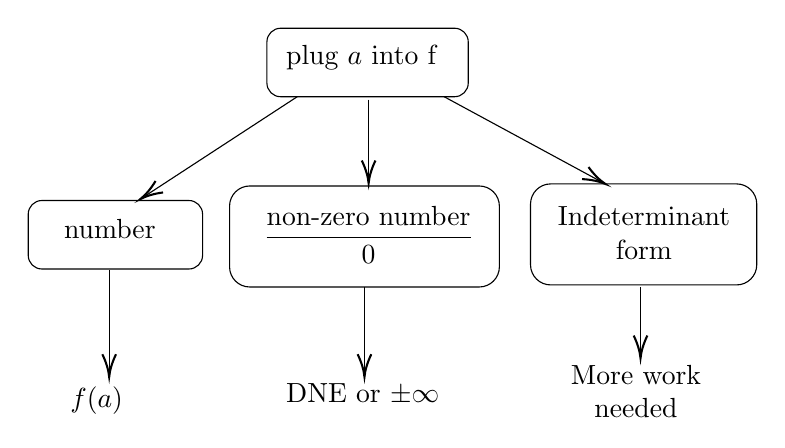
\begin{tikzpicture}[x=0.75pt,y=0.75pt,yscale=-1,xscale=1]
%uncomment if require: \path (0,446); %set diagram left start at 0, and has height of 446

%Rounded Rect [id:dp04536261924917495] 
\draw   (218,91.93) .. controls (218,88.29) and (220.95,85.33) .. (224.6,85.33) -- (308.4,85.33) .. controls (312.05,85.33) and (315,88.29) .. (315,91.93) -- (315,111.73) .. controls (315,115.38) and (312.05,118.33) .. (308.4,118.33) -- (224.6,118.33) .. controls (220.95,118.33) and (218,115.38) .. (218,111.73) -- cycle ;
%Straight Lines [id:da43038695232156465] 
\draw    (232.6,118.33) -- (158.67,166.57) ;
\draw [shift={(157,167.67)}, rotate = 326.87] [color={rgb, 255:red, 0; green, 0; blue, 0 }  ][line width=0.75]    (10.93,-3.29) .. controls (6.95,-1.4) and (3.31,-0.3) .. (0,0) .. controls (3.31,0.3) and (6.95,1.4) .. (10.93,3.29)   ;
%Straight Lines [id:da02535983624938165] 
\draw    (267,119.67) -- (267,158) ;
\draw [shift={(267,160)}, rotate = 270] [color={rgb, 255:red, 0; green, 0; blue, 0 }  ][line width=0.75]    (10.93,-3.29) .. controls (6.95,-1.4) and (3.31,-0.3) .. (0,0) .. controls (3.31,0.3) and (6.95,1.4) .. (10.93,3.29)   ;
%Straight Lines [id:da33645697944263864] 
\draw    (303.4,118.33) -- (379.24,159.38) ;
\draw [shift={(381,160.33)}, rotate = 208.42] [color={rgb, 255:red, 0; green, 0; blue, 0 }  ][line width=0.75]    (10.93,-3.29) .. controls (6.95,-1.4) and (3.31,-0.3) .. (0,0) .. controls (3.31,0.3) and (6.95,1.4) .. (10.93,3.29)   ;
%Rounded Rect [id:dp8149957234073693] 
\draw   (103,174.93) .. controls (103,171.29) and (105.95,168.33) .. (109.6,168.33) -- (180.4,168.33) .. controls (184.05,168.33) and (187,171.29) .. (187,174.93) -- (187,194.73) .. controls (187,198.38) and (184.05,201.33) .. (180.4,201.33) -- (109.6,201.33) .. controls (105.95,201.33) and (103,198.38) .. (103,194.73) -- cycle ;
%Rounded Rect [id:dp9518200785534192] 
\draw   (200,171.07) .. controls (200,165.69) and (204.36,161.33) .. (209.73,161.33) -- (320.27,161.33) .. controls (325.64,161.33) and (330,165.69) .. (330,171.07) -- (330,200.27) .. controls (330,205.64) and (325.64,210) .. (320.27,210) -- (209.73,210) .. controls (204.36,210) and (200,205.64) .. (200,200.27) -- cycle ;
%Rounded Rect [id:dp5380321492603661] 
\draw   (345,170.07) .. controls (345,164.69) and (349.36,160.33) .. (354.73,160.33) -- (444.27,160.33) .. controls (449.64,160.33) and (454,164.69) .. (454,170.07) -- (454,199.27) .. controls (454,204.64) and (449.64,209) .. (444.27,209) -- (354.73,209) .. controls (349.36,209) and (345,204.64) .. (345,199.27) -- cycle ;
%Straight Lines [id:da980017392599877] 
\draw    (142,202) -- (142,251.33) ;
\draw [shift={(142,253.33)}, rotate = 270] [color={rgb, 255:red, 0; green, 0; blue, 0 }  ][line width=0.75]    (10.93,-3.29) .. controls (6.95,-1.4) and (3.31,-0.3) .. (0,0) .. controls (3.31,0.3) and (6.95,1.4) .. (10.93,3.29)   ;
%Straight Lines [id:da24546083605149582] 
\draw    (265,210) -- (265,251.33) ;
\draw [shift={(265,253.33)}, rotate = 270] [color={rgb, 255:red, 0; green, 0; blue, 0 }  ][line width=0.75]    (10.93,-3.29) .. controls (6.95,-1.4) and (3.31,-0.3) .. (0,0) .. controls (3.31,0.3) and (6.95,1.4) .. (10.93,3.29)   ;
%Straight Lines [id:da8582799815353812] 
\draw    (398,210) -- (398,242.33) ;
\draw [shift={(398,244.33)}, rotate = 270] [color={rgb, 255:red, 0; green, 0; blue, 0 }  ][line width=0.75]    (10.93,-3.29) .. controls (6.95,-1.4) and (3.31,-0.3) .. (0,0) .. controls (3.31,0.3) and (6.95,1.4) .. (10.93,3.29)   ;

% Text Node
\draw (226,92.33) node [anchor=north west][inner sep=0.75pt]   [align=left] {plug $\displaystyle a$ into f};
% Text Node
\draw (119,176.33) node [anchor=north west][inner sep=0.75pt]   [align=left] {number};
% Text Node
\draw (355,170) node [anchor=north west][inner sep=0.75pt]   [align=left] {\begin{minipage}[lt]{65.09pt}\setlength\topsep{0pt}
\begin{center}
Indeterminant\\form
\end{center}

\end{minipage}};
% Text Node
\draw (122,256.83) node [anchor=north west][inner sep=0.75pt]   [align=left] {$f(a)$};
% Text Node
\draw (226,255.33) node [anchor=north west][inner sep=0.75pt]   [align=left] {DNE or $\displaystyle \pm \infty $};
% Text Node
\draw (361,246.33) node [anchor=north west][inner sep=0.75pt]   [align=left] {\begin{minipage}[lt]{50.33pt}\setlength\topsep{0pt}
\begin{center}
More work\\needed
\end{center}

\end{minipage}};
% Text Node
\draw (215,170) node [anchor=north west][inner sep=0.75pt]    {$\displaystyle\frac{\text{non-zero number}}{0}$};

\end{tikzpicture}
    }
    \caption{Flowchart for evaluating limits}
    \label{fig:flowchart}
\end{figure}

\subsection{A Number}

If $f$ is an ACCF and $f(a)$ is a number, then $a$ is in the domain of $f$. Since any ACCF is continuous on its domain,
$$\lim_{x\to a}f(x)=f(a)$$
by the definition of continuity. \mar{Re-read this until you understand it!}

\subsection{A (non-zero) Number over Zero}

If $f$ is an ACCF and attempting to evaluate $f(a)$ results in a non-zero number over 0, then $f$ has a vertical asymptote at $x=a$. Near $x=a$, the values of $f(x)$ get very close to either positive or negative infinity. The right and left sided limits are either positive or negative infinity, so there are only four cases, as seen in figure \ref{fig:four-cases}.

\begin{figure}[h]
    \centering
    \fbox{
        \resizebox{4.25in}{!}{
        \tikzset{every picture/.style={line width=0.75pt}} %set default line width to 0.75pt        
        
        \begin{tikzpicture}[x=0.75pt,y=0.75pt,yscale=-1,xscale=1]
        %uncomment if require: \path (0,446); %set diagram left start at 0, and has height of 446
        
        %Straight Lines [id:da7130638550602129] 
        \draw    (17.32,128.98) -- (162.73,128.98) ;
        %Curve Lines [id:da8198586763402247] 
        \draw    (19.1,124.51) .. controls (81.55,124.51) and (86.01,102.21) .. (86.01,57.6) ;
        %Curve Lines [id:da33054163491632704] 
        \draw    (161.84,124.51) .. controls (99.39,124.51) and (94.93,102.21) .. (94.93,57.6) ;
        %Straight Lines [id:da39635263385432795] 
        \draw  [dash pattern={on 0.84pt off 2.51pt}]  (90.47,54.93) -- (90.47,201.24) ;
        
        %Straight Lines [id:da4984898910131832] 
        \draw    (187.51,128.98) -- (332.93,128.98) ;
        %Curve Lines [id:da12653349982399664] 
        \draw    (189.3,124.51) .. controls (251.75,124.51) and (256.21,102.21) .. (256.21,57.6) ;
        %Curve Lines [id:da6963380775085903] 
        \draw    (332.04,133.14) .. controls (269.59,133.14) and (265.13,155.74) .. (265.13,200.05) ;
        %Straight Lines [id:da5434138892345324] 
        \draw  [dash pattern={on 0.84pt off 2.51pt}]  (260.67,54.93) -- (260.67,201.24) ;
        
        %Straight Lines [id:da6992946751383504] 
        \draw    (357.71,128.98) -- (503.13,128.98) ;
        %Curve Lines [id:da5321156852218221] 
        \draw    (359.5,132.54) .. controls (421.95,132.54) and (426.41,155.74) .. (426.41,200.05) ;
        %Curve Lines [id:da8818577355654187] 
        \draw    (502.24,124.51) .. controls (439.79,124.51) and (435.33,102.21) .. (435.33,57.6) ;
        %Straight Lines [id:da23325172919339887] 
        \draw  [dash pattern={on 0.84pt off 2.51pt}]  (430.87,54.93) -- (430.87,201.24) ;
        
        %Straight Lines [id:da2808110791577314] 
        \draw    (527.91,128.98) -- (673.33,128.98) ;
        %Curve Lines [id:da43641618110544544] 
        \draw    (530,133.73) .. controls (592.45,133.73) and (596.91,155.14) .. (596.91,200.05) ;
        %Curve Lines [id:da16583705050218067] 
        \draw    (672.44,133.14) .. controls (609.99,133.14) and (605.53,155.74) .. (605.53,200.05) ;
        %Straight Lines [id:da9264659475889601] 
        \draw  [dash pattern={on 0.84pt off 2.51pt}]  (601.07,54.93) -- (601.07,201.24) ;
        
        
        
        
        
        \end{tikzpicture}
        
        % \resizebox{3in}{!}{
        % \tikzset{every picture/.style={line width=0.75pt}} %set default line width to 0.75pt        
        % \begin{tikzpicture}[x=0.75pt,y=0.75pt,yscale=-1,xscale=1]
        % %uncomment if require: \path (0,446); %set diagram left start at 0, and has height of 446
        
        % %Straight Lines [id:da11666177611802953] 
        % \draw    (98,120.33) -- (261,120.33) ;
        % %Curve Lines [id:da20823749405635383] 
        % \draw    (100,115.33) .. controls (170,115.33) and (175,90.33) .. (175,40.33) ;
        % %Curve Lines [id:da5857981133236727] 
        % \draw    (260,115.33) .. controls (190,115.33) and (185,90.33) .. (185,40.33) ;
        % %Straight Lines [id:da8270643292998765] 
        % \draw  [dash pattern={on 0.84pt off 2.51pt}]  (180,37.33) -- (180,201.33) ;
        
        % %Straight Lines [id:da6737028355731796] 
        % \draw    (288,120.33) -- (451,120.33) ;
        % %Curve Lines [id:da5853120673537593] 
        % \draw    (290,115.33) .. controls (360,115.33) and (365,90.33) .. (365,40.33) ;
        % %Curve Lines [id:da33546715055487053] 
        % \draw    (450,125) .. controls (380,125) and (375,150.33) .. (375,200) ;
        % %Straight Lines [id:da39333458455778736] 
        % \draw  [dash pattern={on 0.84pt off 2.51pt}]  (370,37.33) -- (370,201.33) ;
        
        
        % %Straight Lines [id:da41843468171367526] 
        % \draw    (98,310.33) -- (261,310.33) ;
        % %Curve Lines [id:da9482877395734075] 
        % \draw    (100,314.33) .. controls (170,314.33) and (175,340.33) .. (175,390) ;
        % %Curve Lines [id:da7803855380541431] 
        % \draw    (260,305.33) .. controls (190,305.33) and (185,280.33) .. (185,230.33) ;
        % %Straight Lines [id:da11027576459803168] 
        % \draw  [dash pattern={on 0.84pt off 2.51pt}]  (180,227.33) -- (180,391.33) ;
        
        % %Straight Lines [id:da294114983098098] 
        % \draw    (288,310.33) -- (451,310.33) ;
        % %Curve Lines [id:da491751074451225] 
        % \draw    (290.33,315.67) .. controls (360.33,315.67) and (365.33,339.67) .. (365.33,390) ;
        % %Curve Lines [id:da32646541541064433] 
        % \draw    (450,315) .. controls (380,315) and (375,340.33) .. (375,390) ;
        % %Straight Lines [id:da20001269749677508] 
        % \draw  [dash pattern={on 0.84pt off 2.51pt}]  (370,227.33) -- (370,391.33) ;
        
        
        
        
        
        
        % \end{tikzpicture}
        % }
        }
    }
    \caption{The four cases of vertical asymptotes}
    \label{fig:four-cases}
\end{figure}

Therefore, the only possibilities for the value of these limits are $\infty$, $-\infty$, and DNE. \mar{Label each function in figure \ref{fig:four-cases} with its respective limit.} To figure it out which one it is, evaluate both of the two sided limits. For each, plug in a value that is slightly to the right (or the left) of $a$. If the result is positive, the sided limit is positive infinity, and if the result is negative, negative infinity.

\subsection{Indeterminant Form}

There are seven indeterminant forms:

\vspace{1em}

\begin{center}
\begin{Large}
\phantom{}\hfill
$\frac{0}{0}$ \hfill
$\frac{\infty}{\infty}$ \hfill
$0^0$ \hfill
$\infty{-}\infty$ \hfill
$1^\infty$ \hfill
$0{\cdot}\infty$ \hfill
$\infty^0$
\hfill\phantom{}
\end{Large}
\end{center}

\vspace{1em}

They are called \textbf{indeterminant} because in this form, we cannot be sure of its value (or even if its value makes sense). Take $0^0$ for example: zero raised to any power should be 0, but anything raised to the power of $0$ should be 1... so which is it? \mar{Write out similar question for the other 6 indeterminant forms.}

When we get an indeterminant form after trying to evaluate $f(a)$, we need to do more work. There are several things you can try:

\begin{itemize}
\item Simplify. If the function is rational and has common factor in its numerator and denominator, by ``canceling'' the term, the resulting function is not the same: the original function has a hole at the point where the factored term is 0. For example, $f(x)=\frac{x(x-1)}{(x-1)}$ has a hole at $x=1$, but everywhere else is the line $y=x$. However, this cancellation does not change the value of the limit.
\item Multiply the numerator and denominator of a rational function by the conjugate of the denominator or the numerator (the \textbf{conjugate} of a binomial $a+b$ is $a-b$).
\item Use a special-case limit: 
$$
\lim_{x\to 0}\frac{\sin(x)}{x} = 1
\quad\quad\quad\quad
\lim_{x\to 0}\frac{\cos(x) - 1}{x} = 0
$$
$$
\lim_{x\to\infty}\left(1+\frac{1}{x}\right)^x = e
\quad\quad\quad\quad
\lim_{x\to 0}\frac{a^x-1}{x}=\ln(a)
$$

\item In the case of $x\to\pm\infty$ for a rational function, divide the numerator and denominator by the highest degree term of the denominator.

\item Use the Squeeze Theorem:

\begin{thm}[Squeeze Theorem]
Let $f$, $g$, and $h$ be functions with $g(x)\leq f(x)\leq h(x)$ for all $x$ in some interval around $a$ (except possibly at $a$). If $$\lim_{x\to a}g(x)=L=\lim_{x\to a} h(x),$$ then $$\lim_{x\to a} f(x)=L$$
as well.
\end{thm}
The most common application of squeeze theorem is squeezing $$-1\leq \sin\theta \leq 1.$$

\end{itemize}

Later, we will learn a trick called L'H\^opital's Rule to more easily compute limits with indeterminant forms. But first we need to learn about derivatives!

















\end{document}












